%####################################################################################################################################################
% FYS4580 PROJECT REPORT
%####################################################################################################################################################

\documentclass[twocolumn,a4paper,10pt]{article}

\usepackage{graphicx}
\usepackage{amsmath}
\usepackage{slashed}
\usepackage{enumerate}
\usepackage{hyperref}
\usepackage{array}
\usepackage{multirow}
\usepackage{lipsum,multicol}
\usepackage{dirtytalk}

\renewcommand{\thesubsection}{\Roman{subsection}.}

% Use all allowed space
\addtolength{\hoffset}{-0.5cm}
\addtolength{\textwidth}{1.0cm}
\addtolength{\voffset}{-1.5cm}
\addtolength{\textheight}{0.15\textwidth}
\setlength{\columnsep}{0.5cm}

\author{Kevin Cappa \\ University of Oslo}

\title{{\huge FYS4580 - Semester Project Fall 2024} \\ 
        \noindent\rule[5pt]{12cm}{0.4pt} \\
        From Fuel Pin Cell to Reactor Core Design of APWRs \\
        A 13-Month Cycle Depletion Simulation with OpenMC} %Anatomy

\begin{document}

%####################################################################################################################################################
% ABSTRACT
%####################################################################################################################################################

\twocolumn[
\begin{@twocolumnfalse}
  \maketitle
  \begin{abstract}
    In this report we will discuss the basic structure of an advanced pressurized water reactor (APWR) for a model simulation in OpenMC. The report will follow the overarching structure of the FYS4590 project description for the Fall semester 2024. After defining the materials and the geometry of the reactor we will delve deeper in to the underlaying reactor physics of the model through a depletion calculation and laslty we will discuss the obtained results.
  \end{abstract}
  \vspace{5mm}
\end{@twocolumnfalse}
]

%####################################################################################################################################################
% ESSAY
%####################################################################################################################################################

%####################################################################################################################################################
% 1 - INTRODUCTION
%####################################################################################################################################################

\section{Introduction}

\par
The main scope of this project report is to give a thourough, albeit simple, overview of introductory reactor physics applied to a rudimentary reactor core simulation. We will show how to build a modern advanced pressurized reactor (APWR) from its basic building block, the pin cell, to its outermost layer, the reactor pressure vessel, and give a brief discussion on how such a reactor differ from the usual pressurized water reactor (PWR). We will go into detail about the composition of the different pin cells that constitute the APWR, the assembly and core geometry and finally go through a depletion calculation in section~\ref{sec:Simulation}. This will aid us in discussing key points about criticality, fuel burnup, the conversion of uranium-235 to plutonium-239 in the reactor core, in addition to see how the chosen geometry and composition influences the the different factors in the four/five factors formula. This setup has been inspired by a paper published by K. Seki et.al. at the 2003 IAEA/INIS ``International conference on global environment and advanced nuclear power plants" organized by the Atomic Energy Society of Japan in Kyoto, Japan~\cite{APWR}. Although, due to the usual lack of detailed information in publicly published papers on nuclear reactor cores' designs, we decided to extend the geometry by implementing a typical assembly configuration for reactors containing burnup fuels like gadolinia~\cite{BurnupFuel}. In the end a concise discussion of the pros and cons of this type of reactors will be explored in section~\ref{sec:Results and Discussion}. Lastly, we will give an outline of the accuracy of our model and simulation, possibles improvements and furhter developments in section~\ref{sec:Conclusion}. The source code for the simulation can be found in the author's GitHub folder~\cite{GitHub}.

%####################################################################################################################################################
% 2 - SIMULATION
%####################################################################################################################################################

\section{OpenMC Simulation}
\label{sec:Simulation}

\subsection[Materials and Geometry]{\centering Materials and Geometry}
\label{subsec:Materials and Geometry}

\par
The basic building block of a nuclear reactor design is the fuel pin cell. In our case, for the chosen reactor design of the proposed japanese APWR, we have several kinds of pin cells inside the reactor core. Firstly we built the fuel pin cell, made of three concentric cylindrical layers. The innermost cylinder is the fuel pellet, composed of uranium dioxide ($UO_2$), with a 4.8\% $^{235}_{92}U$ enrichment, with a radius of 4,45 mm and height of 36,6 mm. The next layer has a thickness of 0.2 mm and is filled with helium gass. This is done in order to accomodate for the fuel pellet thermal expansion. The outermost layer is a 0.3 mm thick cladding made of zyrcaloy-4, an alloy made up of 98.5\% zyrconium $(_{40}Zr)$ and 1.5\% tin $(_{50}Sn)$. The fuel pin cell is immersed in a box containing borated water, in this case is a 1\% boric acid ($B(OH)_3$) with 10\% boron $^{10}_{5}B$ concentration, in a light water $(H_2O)$ suspension. This setup can be seen in Fig.~\ref{fig:fuelpinxy} and Fig.~\ref{fig:fuelpinyz}, where the uranium dioxide is colored in neon green, the helium is yellow, the zircaloy is light gray and the borated water is deep blue. Similarly, we have defined a burnable fuel pin cell: the burnable fuel pellet contains the burnable absober gadolinium oxide $Gd_2O_3$ with different isotope amounts gadolinium \cite{BurnupFuel} in addition to the previously defined uranium oxide. This has been defined as a mixed oxide (MOX) fuel pellet. The addition of the burnable absorber serves mainly to reduce radioactive waste and reactivity penalties, and to enhance the capability of core reactivity \cite{APWR}. This setup can be seen in Fig.~\ref{fig:burnfuel_xy} and Fig.~\ref{fig:burnfuel_yz}, where the mox fuel is colored in hot pink.

% FIGURE: Top view of the fuel pin cell
\begin{figure}[ht]
  \centering
  \includegraphics[width=0.4\textwidth]{../Pictures/Fuelrods_plot_xy.png}
  \caption{Top view of the fuel pin cell.}
  \label{fig:fuelpinxy}
\end{figure}

% FIGURE: Side view of the fuel pin cell
\begin{figure}[ht]
  \centering
  \includegraphics[width=0.4\textwidth]{../Pictures/Fuelrods_plot_yz.png}
  \caption{Side view of the fuel pin cell.}
  \label{fig:fuelpinyz}
\end{figure}

\par
Following the same procedure we defined the control pin cell where, instead of the fuel pellets, the innermost cylinder is filled with boron carbide (B$_4$C) which is an effective neutron absorber and will help regulate the reactivity in our reactor, see Fig.~\ref{fig:controlpin_xy} and Fig.~\ref{fig:controlpin_yz}. The control pin cell is the inserted in a guiding thimble of radius 0.49 mm, made of stainless steel, see Fig.~\ref{fig:guidepin_xy} and Fig.~\ref{fig:guidepin_yz}. When these guiding tubes are not filled with control elements they are usually filled with air and used for the insertion of control rods and instrumentation inside the reactor core. The materials defined for this model are listed in table \ref{table:materials}.

% TABLE: Materials Table
\begin{table}[t]
\centering
\begin{tabular}{|m{2.7cm}<{\raggedright}||m{2cm}<{\raggedright}|m{1.3cm}<{\raggedright}|}
  \hline
  \multicolumn{3}{|c|}{Materials Table} \\
  \hline
  \hline
  Material              &     Enrichment                                  & Density $[g/cm3]$   \\
  \hline
  \hline
  Uranium dioxide       &     4.8\% U235, 95.2\% U238                     & 10.98               \\
  \hline
  Gadolinium oxide      &     40.0\% Gd, 60.0\% O                         &  7.07               \\
  \hline
  MOX fuel              &     90.0\% UO$_2$, 10.0\% Gd$_2$O$_3$           &  10.589             \\
  \hline
  Boron Carbide         &     80.0\% B, 20.0\% C                          &  2.5                \\
  \hline
  Zircaloy-4            &     98.5\% Zr, 1.5\% Sn                         & 6.56                \\
  \hline
  Helium                &     100.0\% He                                  & 1.78e-6             \\
  \hline
  Graphite              &     100.0\% C                                   & 1.85                \\
  \hline
  Stainless stell       &     86.86\% Fe, 2.14\% C, 11.0\% Cr             &  8.05               \\
  \hline
  Light water           &     66.6\% H, 33.3\% O                          &  1                  \\
  \hline
  Boric acid            &     2.8\% B10, 11.4\% B11, 42.8\% O, 42.8\% H   & 1.435               \\
  \hline
  Borated water         &     1\% B(OH)$_3$, 99\% H$_2$O                  & 1.00435             \\
  \hline
  Air                   &     79.0\% N, 21.0\% O                          &  0.001293           \\
  \hline
\end{tabular}
\caption{Materials used in our OpenMc simulation. Where the isotope number is not specified a natural distribution for the isotopes of the element is assumed. In the case of Gadolinia a specific distribution of the isotope has been chosen following\cite{BurnupFuel}, this can be seen in the source code ``Materials" section.}
\label{table:materials}
\end{table}

\par
The next step is to arrange the defined pin cell into a fuel assembly. This assembly consists of a $17 \times 17$ grid of pin cells stacked above eachother 100 times. This makes all of the pin cell previosuly defined into 3,66 m long rods. The whole assembly measures roughly $20.5 \times 20.5 \times 366$ cm. Since Seki et al. \cite{APWR} did not provide detailed information about the assembly configuration we decided to include in our model an assembly configuration proposed by Hesketh \cite{BurnupFuel}, as shown in Fig.~\ref{fig:fuelass_xy} and Fig.~\ref{fig:fuelass_yz}. The 236 lime green pin cell are the regular UO$_2$ fuel pin cells, the 28 hot pink pin cells are the Gd$_2$O$_3$-UO$_2$ MOX fuel pin cells and the24  white pin cells are the control/guide thimbles filled with air. As seen in Fig.~\ref{fig:fuelass_yz} the B$_4$C control rods are inserted 25\% of the assembly height while the remaining 75\% of the guide thimbles are filled with air. The central guiding thimble is reserved for instrumentation and is therefore only filled with air. 

% FIGURE: Top view of the fuel assembly
\begin{figure}[ht]
  \centering
  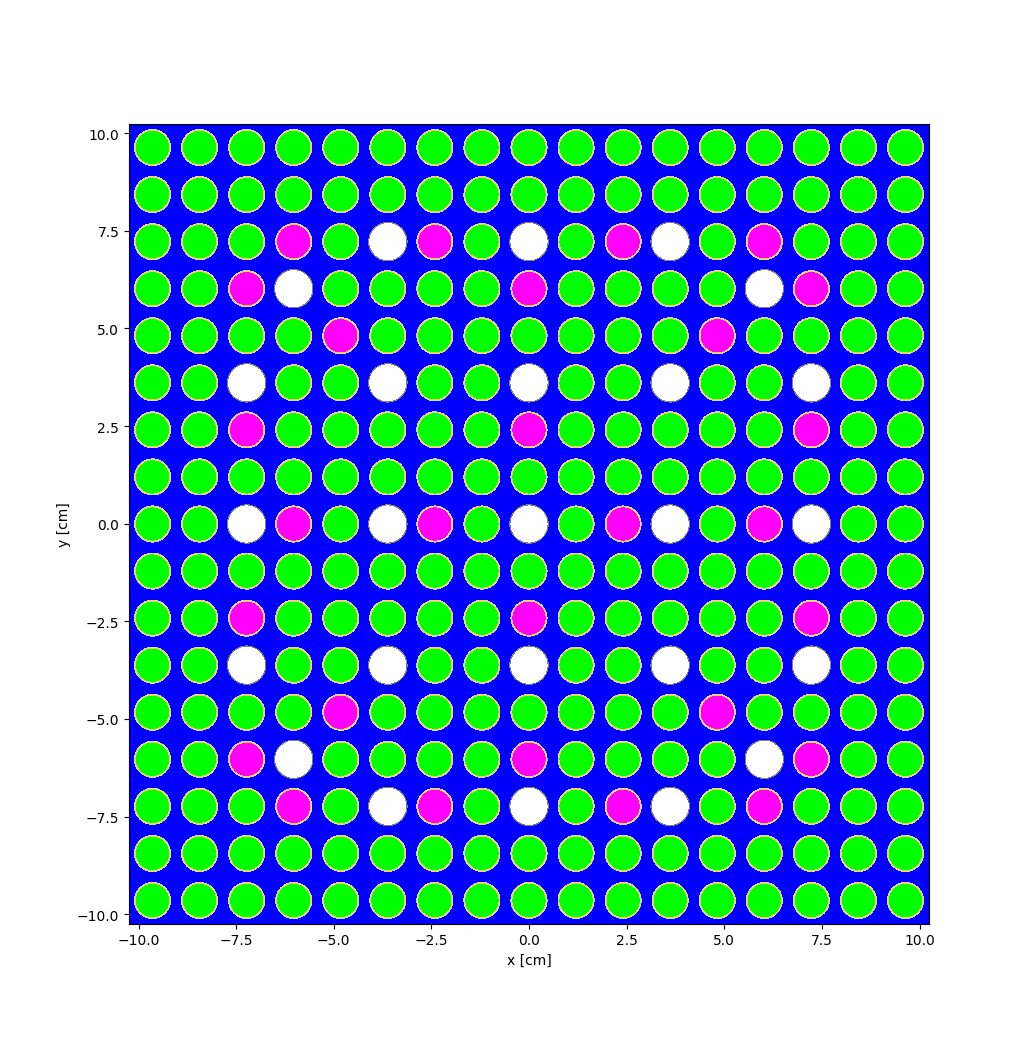
\includegraphics[width=0.4\textwidth]{../Pictures/f_Assembly_Universe_plot_xy.png}
  \caption{Top view of the fuel assembly.}
  \label{fig:fuelass_xy}
\end{figure}

% FIGURE: Side view of the fuel assembly
\begin{figure}[ht]
  \centering
  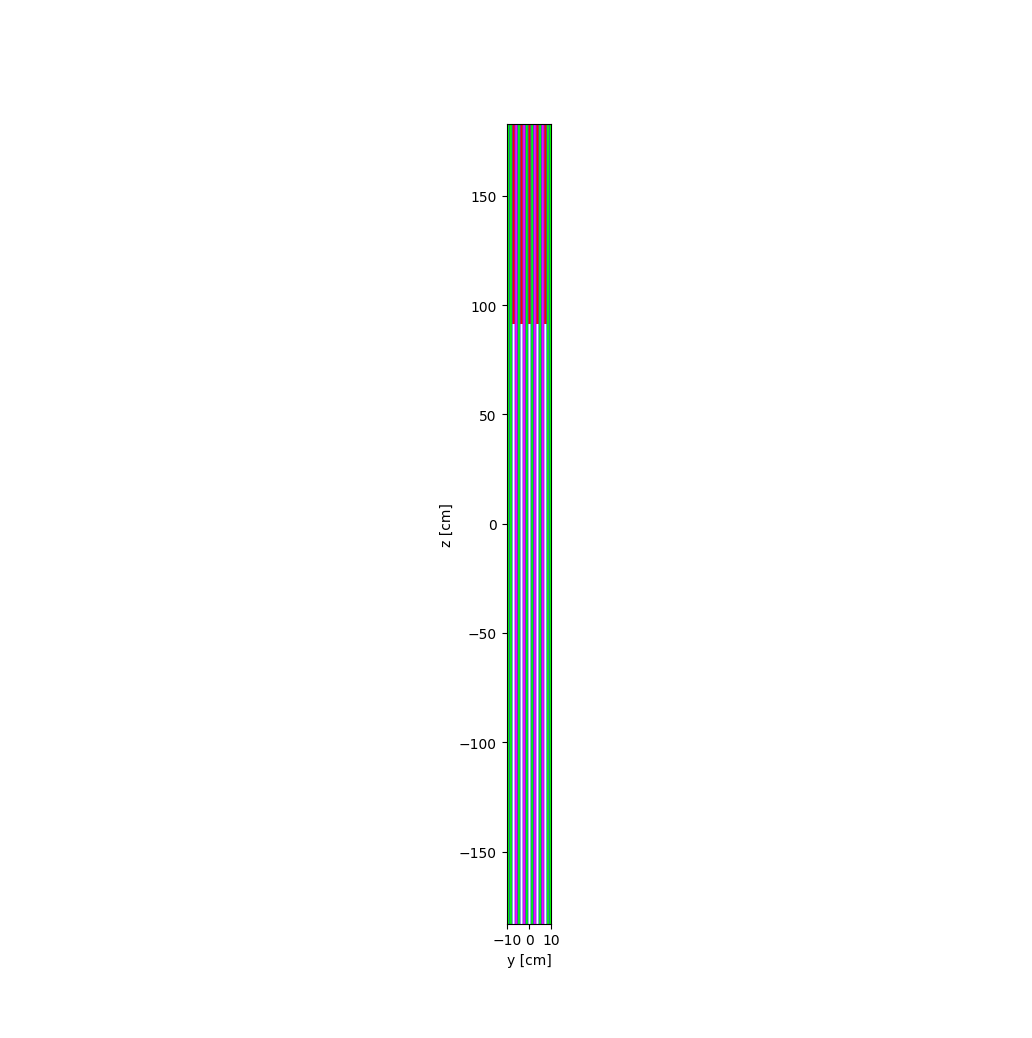
\includegraphics[width=0.4\textwidth]{../Pictures/f_Assembly_Universe_plot_yz.png}
  \caption{Side view of the fuel assembly.}
  \label{fig:fuelass_yz}
\end{figure}

\par
The last step for completing our geometry setup is defining the reactor core and the ractor pressure vessel system. The reactor core is obtained by creating an $17 \times 17$ grid of fuel assemblies, where 8 assemblies have been removed from each of the four corners to make te core into a rough cylinder shape, and 69 of the fuel assemblies have been substituted with control assimeblies, i.e. assemblies mad up of only control rods. The whole of the reacoter core is the enclosed in a neutron reflector of pure graphite, which in turn is enclosed into a reactor tank made of stainless steel, a hollow cylinder og 10 cm thickness. Lastly, the reactor tank in enclosed into the reactor pressure vessel, a 20 cm thick outer cylindrical layer separated from the reactor tank by a 20 cm air gap. This setup can be seen in Fig.~\ref{fig:RPV_xy} and Fig.~\ref{fig:RPV_yz}. 

% FIGURE: Top view of the RPV
\begin{figure}[ht]
  \centering
  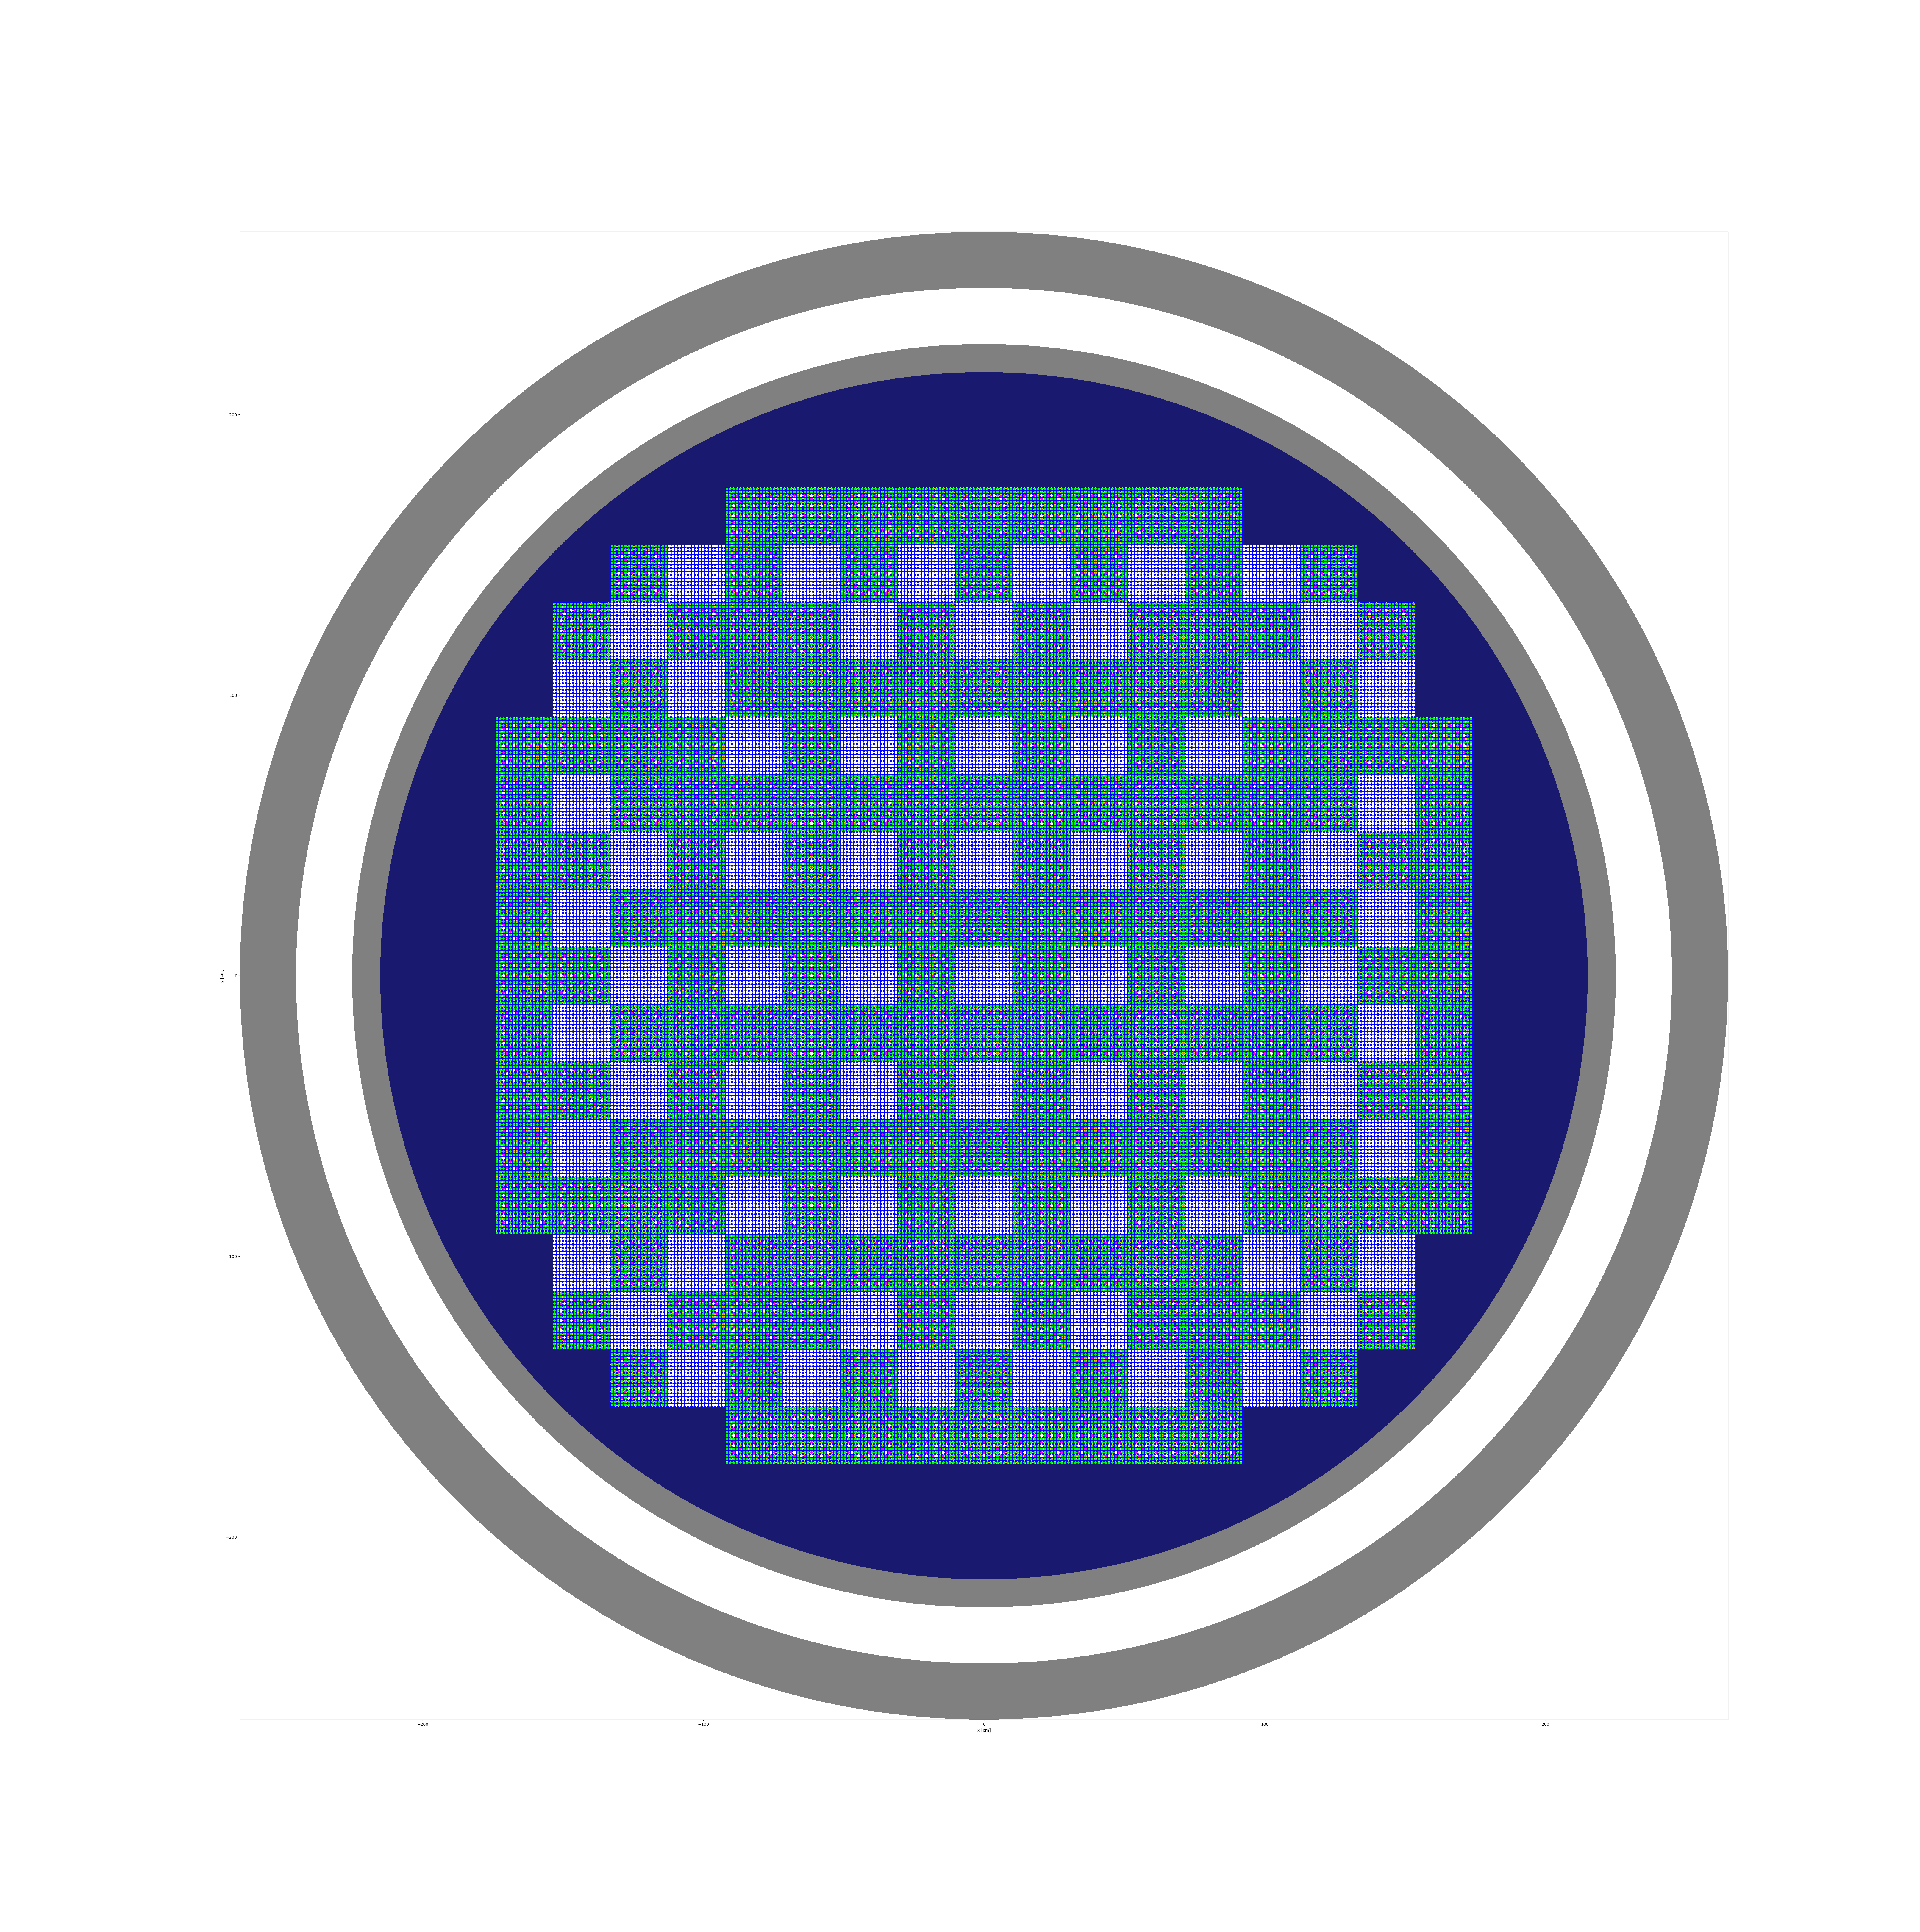
\includegraphics[width=0.4\textwidth]{../Pictures/RPV_Universe_plot_xy.png}
  \caption{Top view of the reactor pressure vessel.}
  \label{fig:RPV_xy}
\end{figure}

% FIGURE: Side view of the RPV
\begin{figure}[ht]
  \centering
  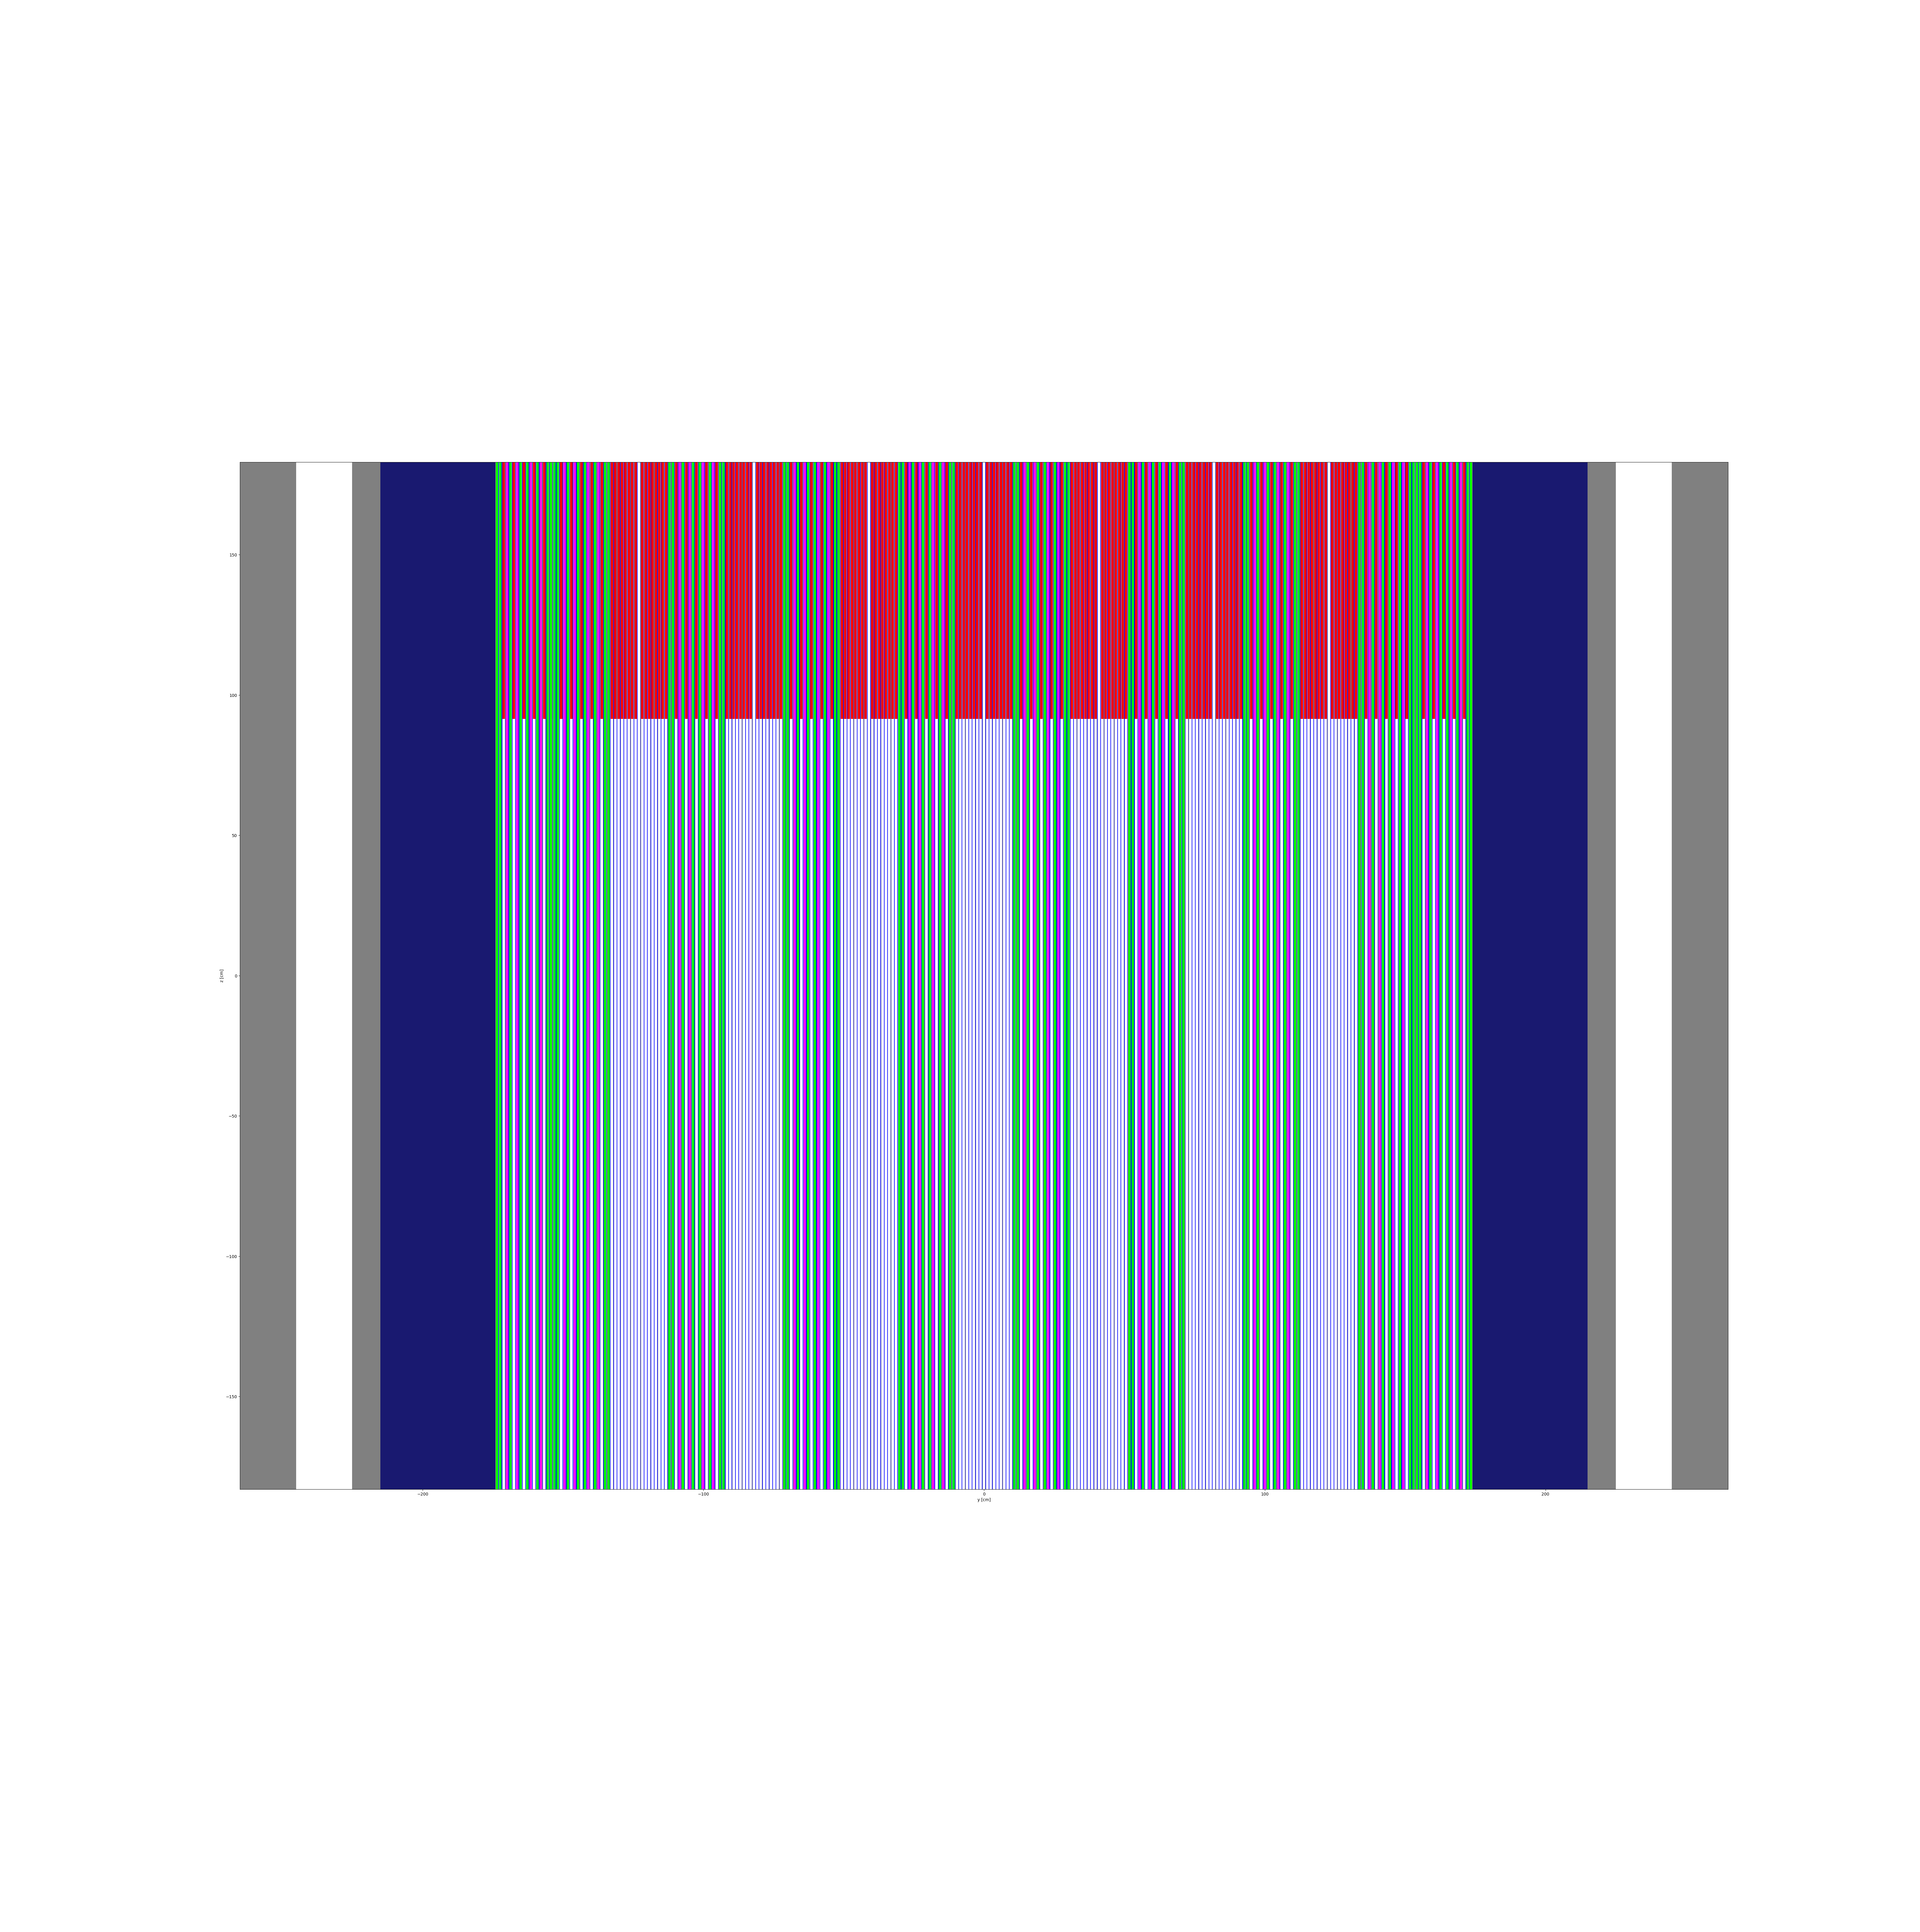
\includegraphics[width=0.4\textwidth]{../Pictures/RPV_Universe_plot_yz.png}
  \caption{Side view of the reactor pressure vessel.}
  \label{fig:RPV_yz}
\end{figure}

\par
This gives us a reactor core that has approximately a 3.49 m diameter and a reactor pressure vessel of roughly 3,8 m in diameter, as specified by the referenced paper \cite{APWR}.\\ \par
For the simple purpose of this project, no top or bottom elements have been designed for the reactor pressure vessel, since in practical applications would differ greatly from what is achievable at this level of OpenMc simulation. Further, it is worth noting that out control rods' design slightly differs from the one proposed by Seki et al. \cite{APWR}, since the design of such elements turned out to be more challenging then expected. This completes our discussion on materials and geomtry used to build our reactor model, and we will now look deeper into the pin cell and reactor k-effective simulation.

\subsection[Pin Cell Simulation]{\centering Pin Cell Simulation}
\label{subsec:Pin Cell Simulation}

\par
We will now take a closer look at the OpenMC fuel pin cell simulation in order to get an approximated value of the neutron multiplication number, i.e. k-effektive, and see how the choice of moderator and fuel pin size can influence the different factors in the five-factor formula and therefore the value of k-effective. All the fuel pin cell simulations we have run in this project follow the geometry outlined for the UO$_2$ fuel pin cell in the previous subsection, and we have focused on changing the boudary conditions of square box containg the fuel pin cell, moderator and size. \\ 

\par
The first OpenMc simulation was run with ``vacuum" boundary conditions, that means that any neutrons passing through the box boundary is lost to the exterior and leaks to the enviroment. In other words the outbound neutrons disappear from our pin cell neutron budged and we therefore expect an extremely subcritical system, i.e. $k_{eff} << 1$. Otherwise, when the same simulation was run for the ``reflective" boundary conditions we expect the neutron multiplication number to increase significantly, and possibly be supercritical. This is because all of the neutrons impinging on the pin cell box boundary will be reflected inwards and has therefore a chance in causing a sustained fission reaction in the fuel. This means in practice that out simple pin cell box behaves like an infinite reactor. The $k_{eff}$ values that have been obtained by these two simulations are registered in table~\ref{table:vacvsref}. 

% TABLE: Boundary conditions
\begin{table}[ht]
\centering
\begin{tabular}{ |m{2.5cm}||m{3.5cm}|}
  \hline
  \multicolumn{2}{|c|}{Boundary conditions} \\
  \hline
  \hline
  Boundary type   &     Combined k-effective  \\
  \hline
  \hline
  Vacuum          &     0.01189 $\pm$ 0.00002   \\
  \hline
  Reflective      &     0.96629 $\pm$ 0.00080   \\
  \hline
\end{tabular}
\caption{Table showing the k-effective values simulated by OpenMC for `` and `` boundary conditions.}
\label{table:vacvsref}
\end{table}

\par
When defining a $100 \times 100$ mesh grid for particle sampling, we can better illustrate the behaviour of the fuel pin cell under such boundary conditions. In Fig.~\ref{fig:vacuum} and Fig.~\ref{fig:reflective} we can see respectively the neutron flux distribution and the fission site heatmap for ``vacuum" and ``reflective" conditions.

% FIGURE: Mesh vacuum
\begin{figure}[ht]
  \centering
  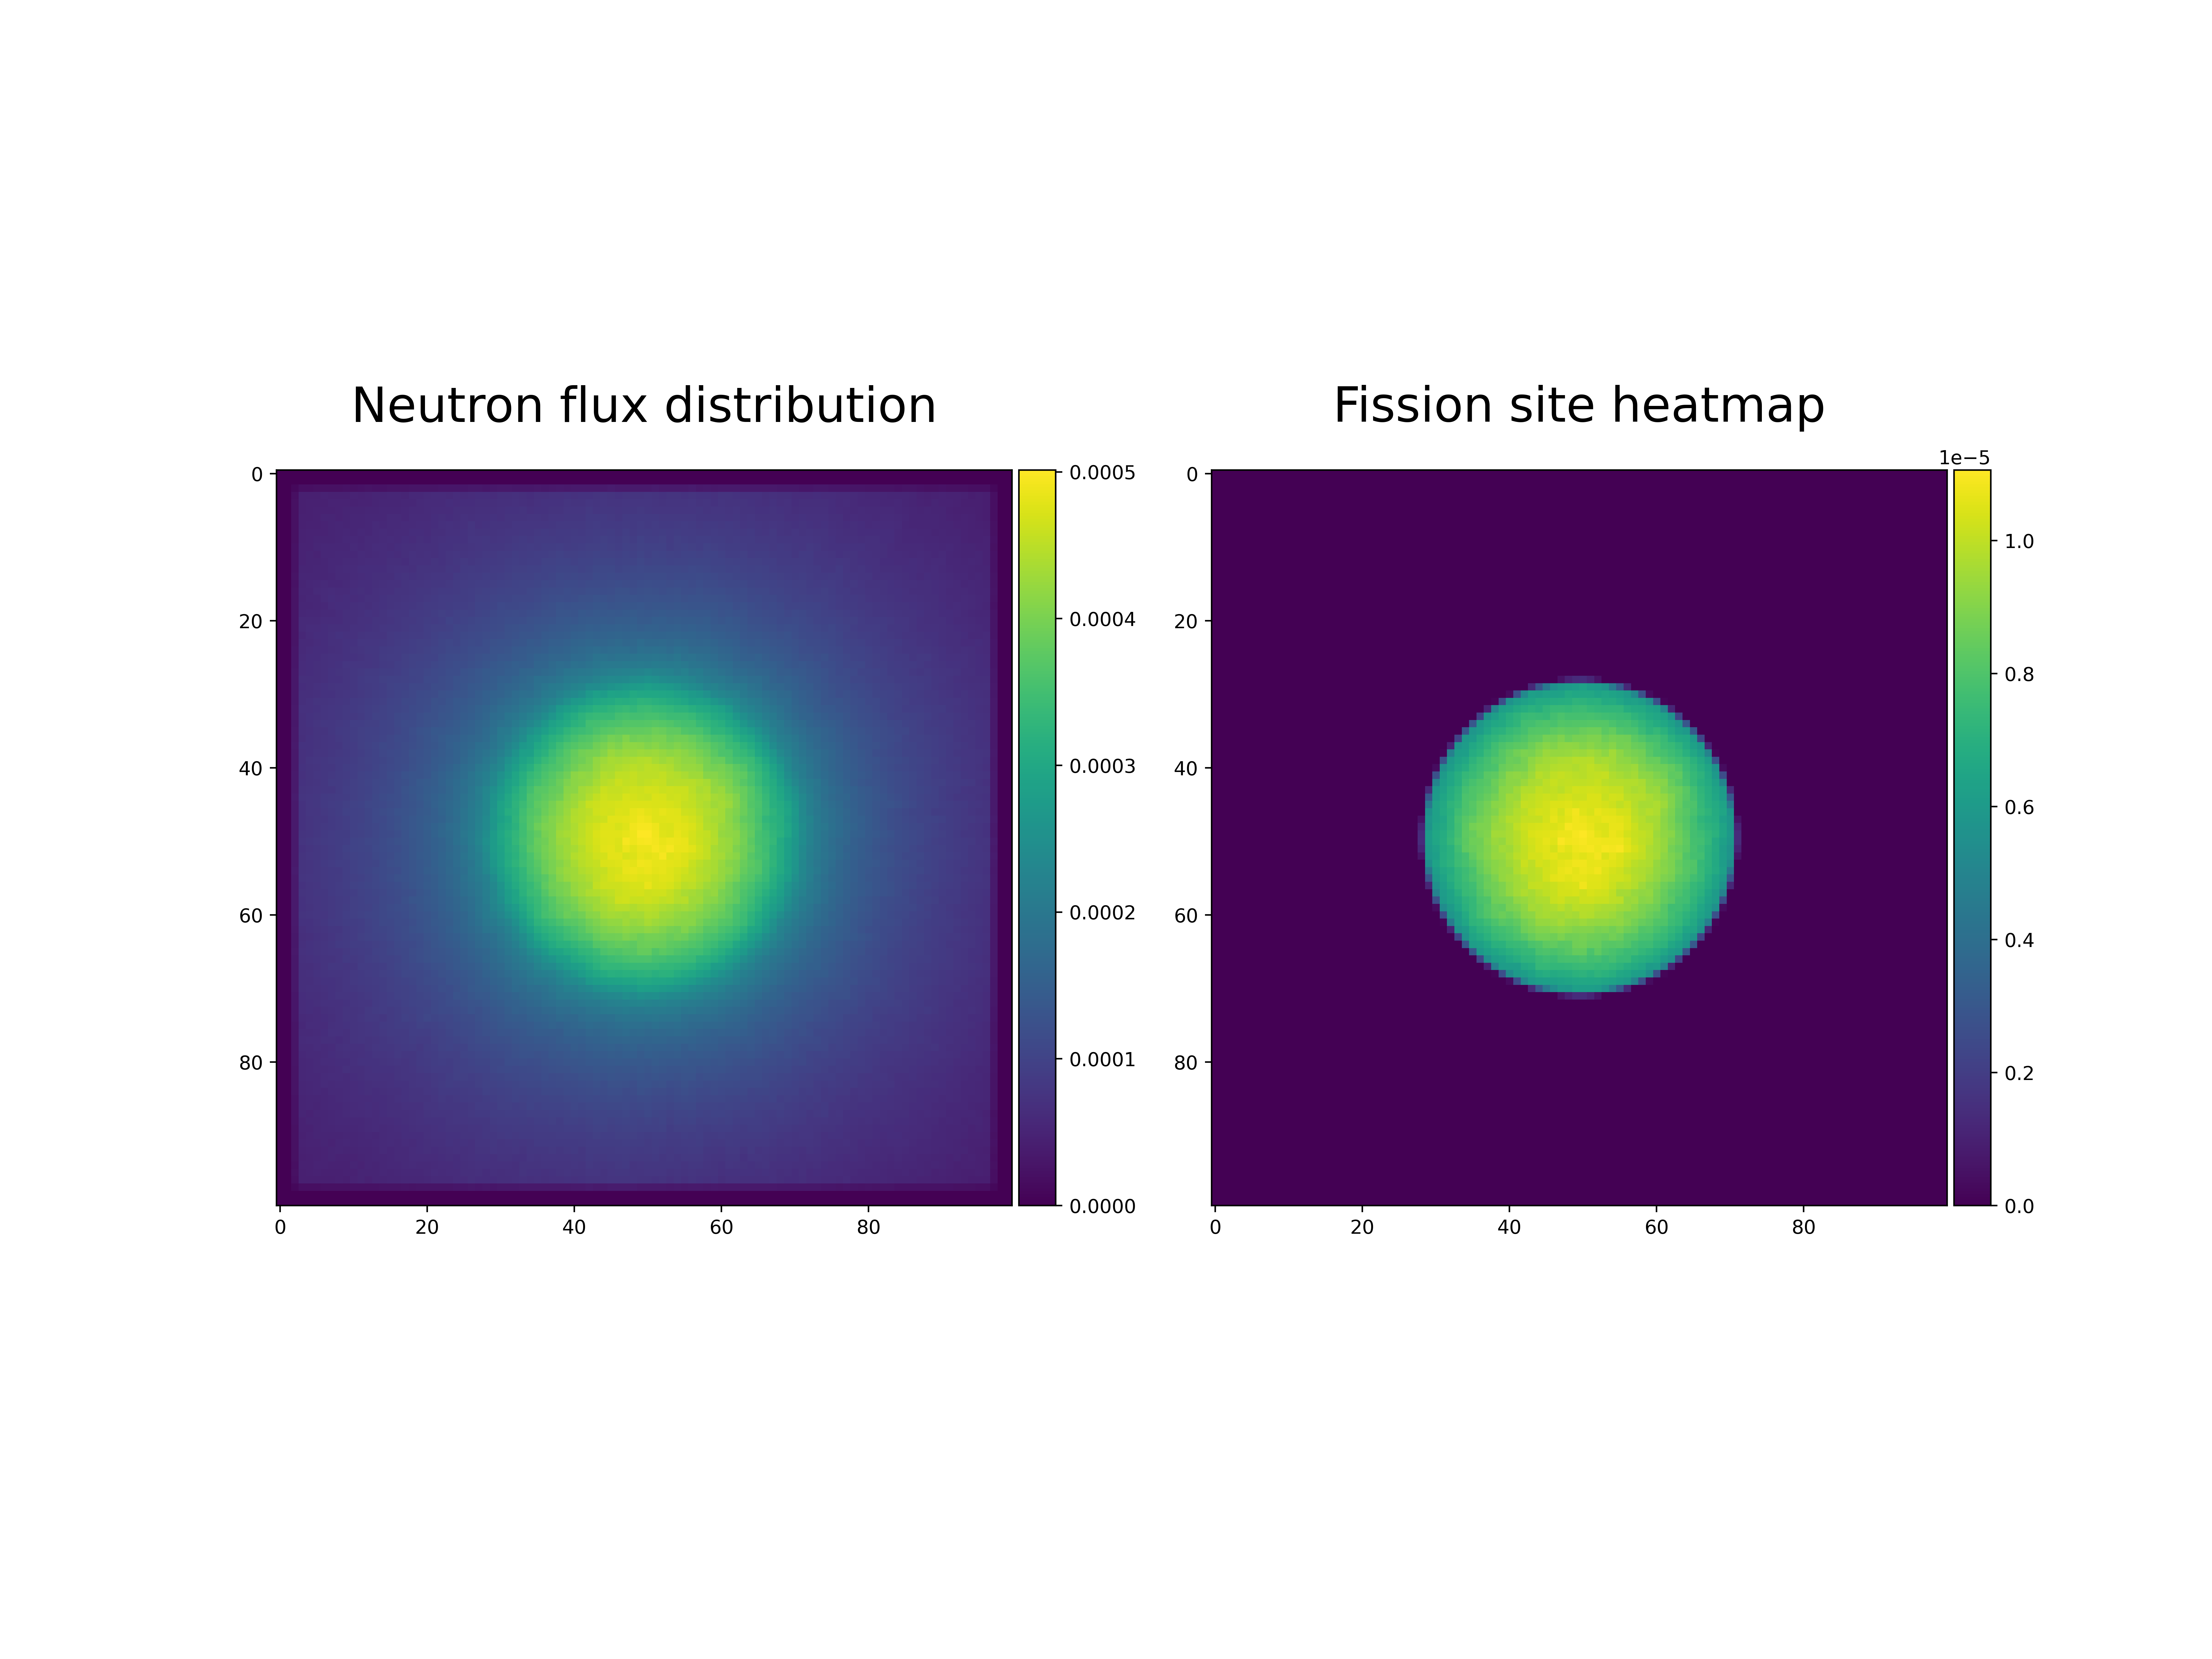
\includegraphics[width=0.4\textwidth]{../Pin_Cell/Mesh_Fuel_Pin_Cell_Vacuum.png}
  \caption{Neutron flux distribution and fission site heatmap for a pin cell with ``vacuum" transmission boundary.}
  \label{fig:vacuum}
\end{figure}

% FIGURE: Mesh reflective
\begin{figure}[ht]
  \centering
  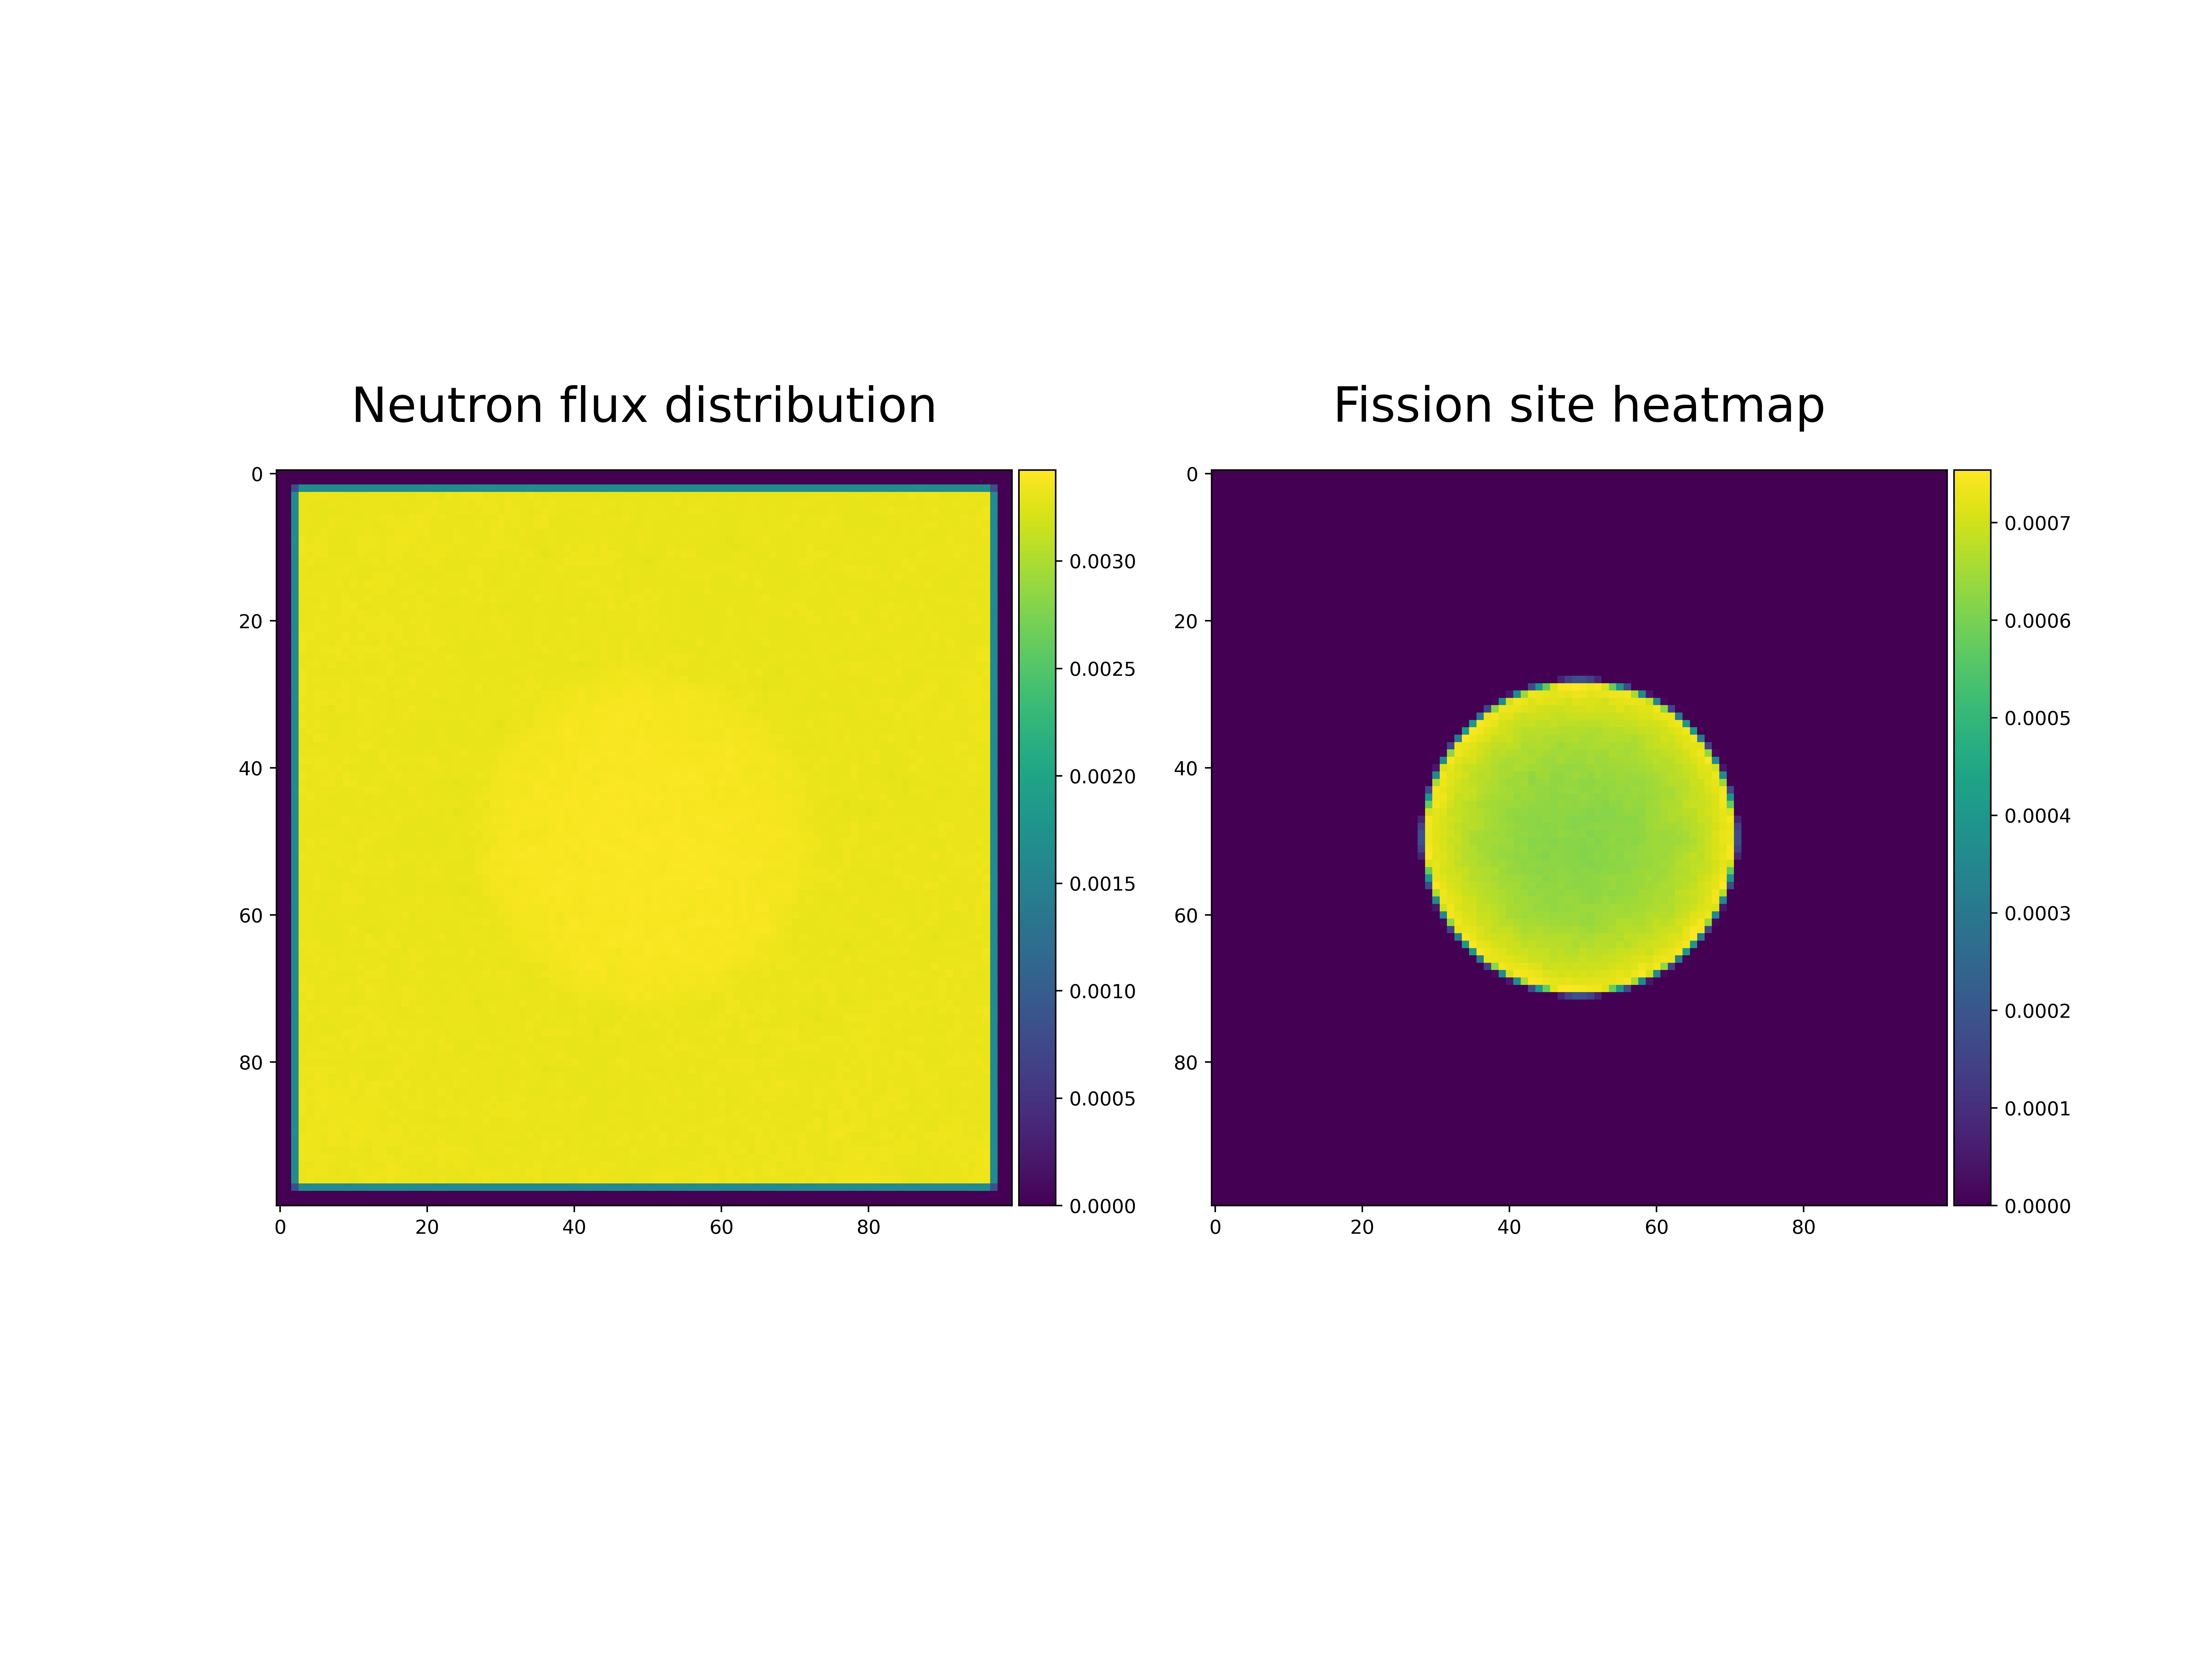
\includegraphics[width=0.4\textwidth]{../Pin_Cell/Mesh_Fuel_Pin_Cell_Reflective.png}
  \caption{Neutron flux distribution and fission site heatmap for a pin cell with ``reflective" transmission boundary.}
  \label{fig:reflective}
\end{figure}

\par
Through OpenMC it is also possible to produce plots for the neutron energy distribution on the eV scale. This has been done for out sample fuel pin cell for both ``vacuum" and ``reflective" boundary conditions. In Fig.~\ref{fig:pincellenergyvac} we can observe that the neutron energy distribution has a peak in the MeV region, a.k.a the fast neutron region; this is presumably due to short path our neutrons travel in the moderator before leaking out of the box and have therefore not managed to be properly moderated in order to reach the eV region and thus become thermal. \\
\par
On the other hand when looking at same energy spectrum for the neutrons in ``reflective" fuel pincell in Fig.~\ref{fig:pincellenergyref}, we can see that there is also a peak in the eV region. This sudden abundance of thermal neutron is most probably due to the better moderation of the promp neutrons, since on average they travel twice as long into the moderator before reaching the ``next" pincell.

% FIGURE: Pin cell energy vacuum
\begin{figure}[ht]
  \centering
  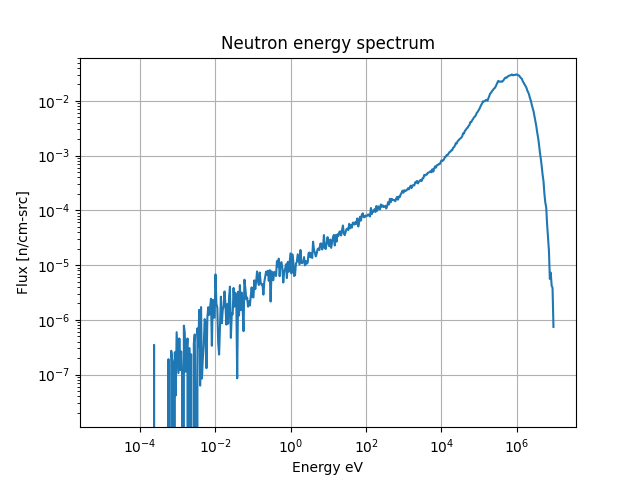
\includegraphics[width=0.4\textwidth]{../Pin_Cell/Energy_Vacuum.png}
  \caption{Neutron energy distribution for a pin cell with ``vacuum" transmission boundary.}
  \label{fig:pincellenergyvac}
\end{figure}

% FIGURE: Pin cell energy reflective
\begin{figure}[ht]
  \centering
  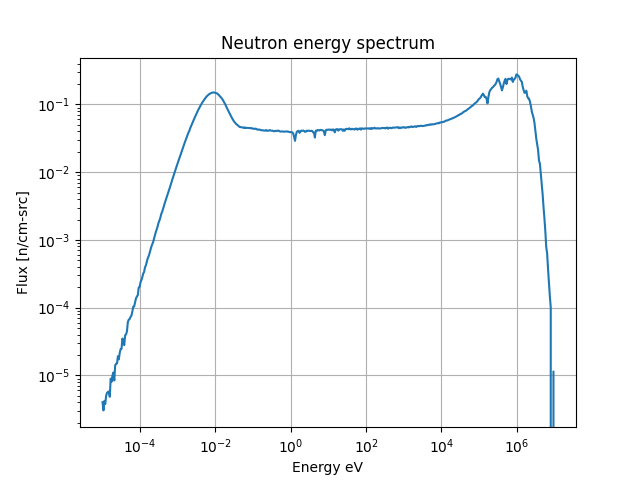
\includegraphics[width=0.4\textwidth]{../Pin_Cell/Energy_Reflective.png}
  \caption{Neutron energy distribution for a pin cell with ``reflective" transmission boundary.}
  \label{fig:pincellenergyref}
\end{figure}

\par
We can now concentrate on the choice of moderator: different moderators mean different capabilities for slowing down the prompt neutrons to the right energy and make them thermal in order to induce more fission. The three standard moderator choices are light water, usually utilized in reactors with enriched uranium fuel, heavy water and graphite, the preferred moderators for reactors with natural uranium fuel. In fact the first nuclear reactor, the Chigago Pile-1 used nuclear graphite as a moderator. Considering our choice of fuel and reactor design, the light water will give better results in order to obtain a critical reactor. (In our case we actually used borated water and considered similar in behaviour to light water due to the low boric acid concentration). In our OpenMC simulation, maintaining the fuel and fuel rod size constant and changing only the moderator yeilded the results shown in table ~\ref{table:moderators}.

% TABLE: Moderator Choice
\begin{table}[ht]
\centering
\begin{tabular}{ |m{2.5cm}||m{3.5cm}|}
  \hline
  \multicolumn{2}{|c|}{Moderator Choice} \\
  \hline
  \hline
  Moderator         &     Combined k-effective  \\
  \hline
  \hline
  Light water       &     0.96629 $\pm$ 0.00080   \\
  \hline
  Heavy water       &     1.16345 $\pm$ 0.00104   \\
  \hline
  Graphite          &     0.76977 $\pm$ 0.00073   \\
  \hline
\end{tabular}
\caption{Test of different moderators in our fuel pin cell and respective k-effektive values.}
\label{table:moderators}
\end{table}

\par
So we see that it is a close call between light water and heavy water in order to obtain criticality, light water being only slightly closer to criticaliy then heavy water.\\
\par
However, when we start varying the fuel rod sizes we get the results shown in Fig.~\ref{fig:FFFlight}, for light water, Fig.~\ref{fig:FFFheavy}, for heavy water, and Fig.~\ref{fig:FFFgraphite} for graphite. In these figures also the changing values of the five-factor formula coefficients have been plotted. Fom this we can see that the optimal solution for optimal criticality is given by light water as moderator and fuel rod size with 1 cm diameter. \\
Now focusing only on the thermal utilization factor for our fuel pin cell at varying rod sizes in light water moderator, we get the plot shown in Fig.~\ref{fig:PCLWkeff}. The thermal utilization factor tells us something about hobe many incoming thermal neutrons go on producing nuclear fission. It follows that an increase in the thermal utilization factor will also result in an increase in the neutron multiplication number k-effective. \\
\par
At this point the reader is reminded that we are currently only looking at a single fuel pin cell with reflective boundaries, making it effectively into an infinte reactor with no possibility of external control and added safety. A more practical, and alas physical exemple, shall prompty follow this subsection, as we will take a look at a whole reactor core enclosed in a neutron reflecore, reactor tank and pressure vessel.

% FIGURE: Pin cell light water keff
\begin{figure}[b]
  \centering
  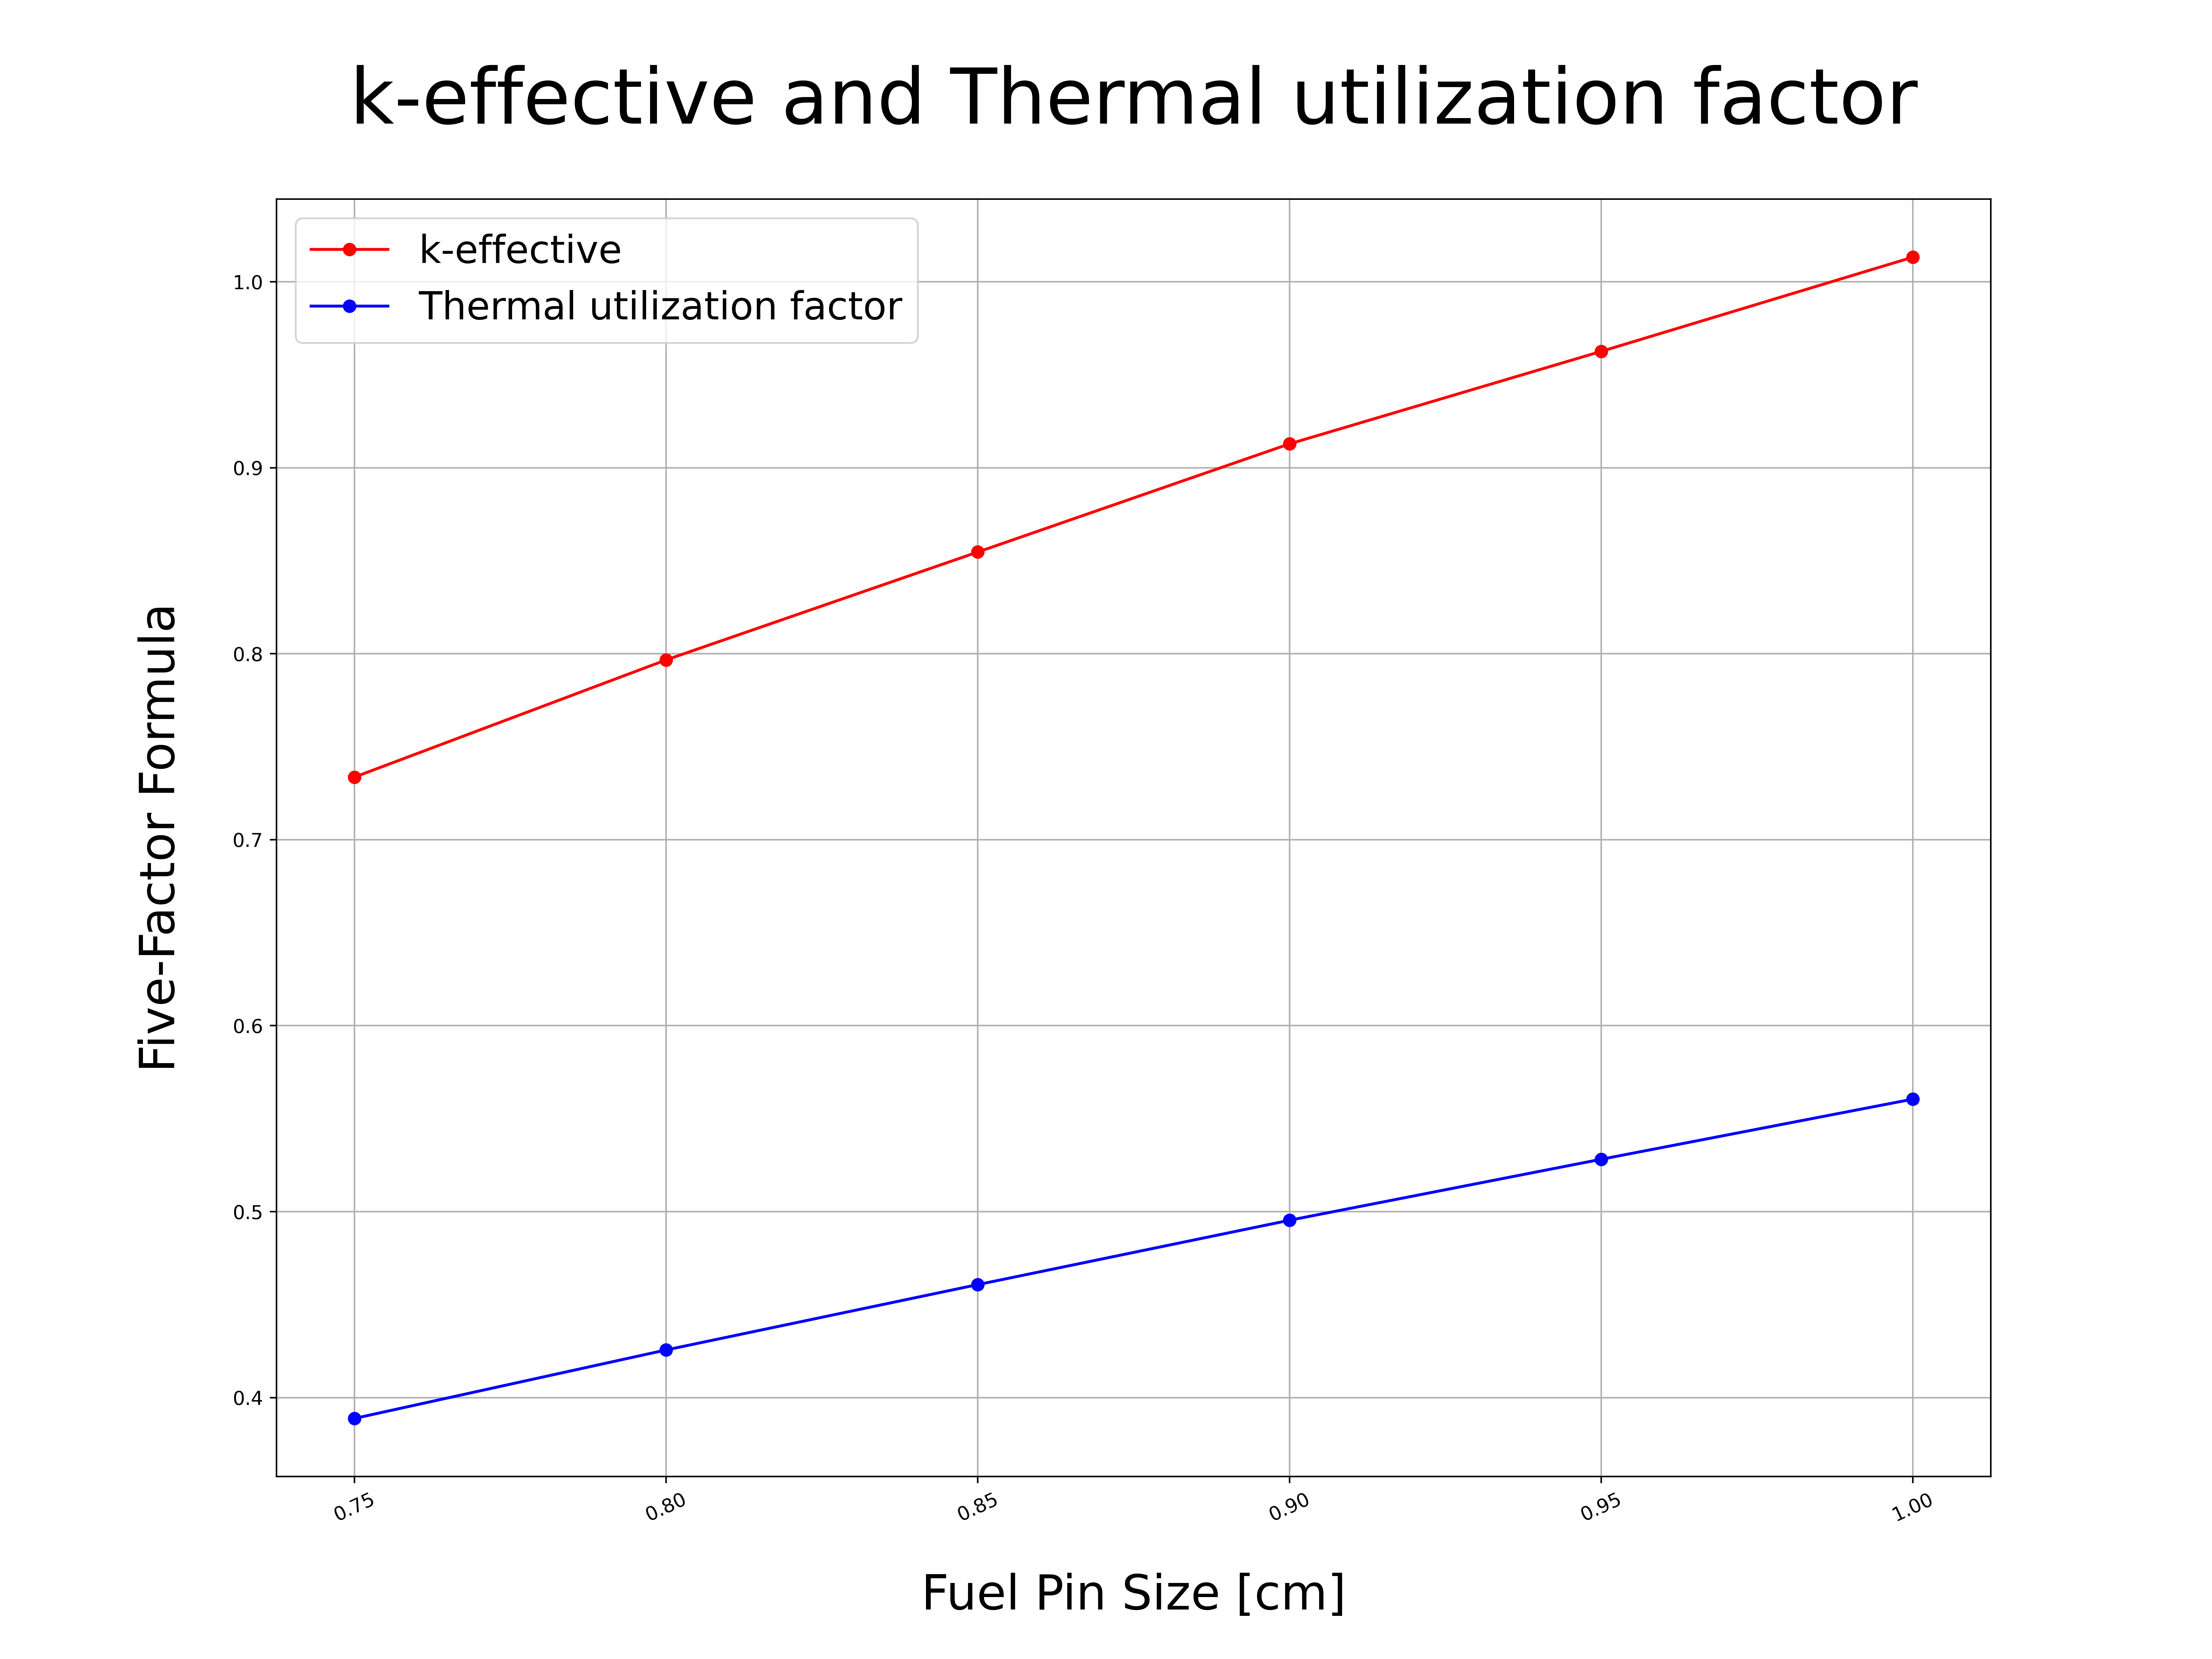
\includegraphics[width=0.4\textwidth]{../Pin_Cell/Light_Water_kandf.png}
  \caption{Thermal utilization factor and k-effective for a pin cell with light water moderator.}
  \label{fig:PCLWkeff}
\end{figure}

\newpage

\subsection[Reactor Core Simulation]{\centering Reactor Core Simulation}
\label{subsec:Reactor Core Simulation}

\par
Following in the footsteps of the pin cell simulation we will now look at the whole reactor as described in subsection~\ref{subsec:Materials and Geometry}. The first change to take into notice is that now the boundary between each material is set to ``transmissive" and only the outedge of the reactor pressure vessel, included the top and the bottom of the reactor, is set to ``vacuum". Reproducing the results obtained from the mesh grid for particle samples of the pin cell adapted for the whole reactor geometry gives us the plot shown in fig.~\ref{fig:meshRPV}.

% FIGURE: Mesh RPV
\begin{figure}[ht]
  \centering
  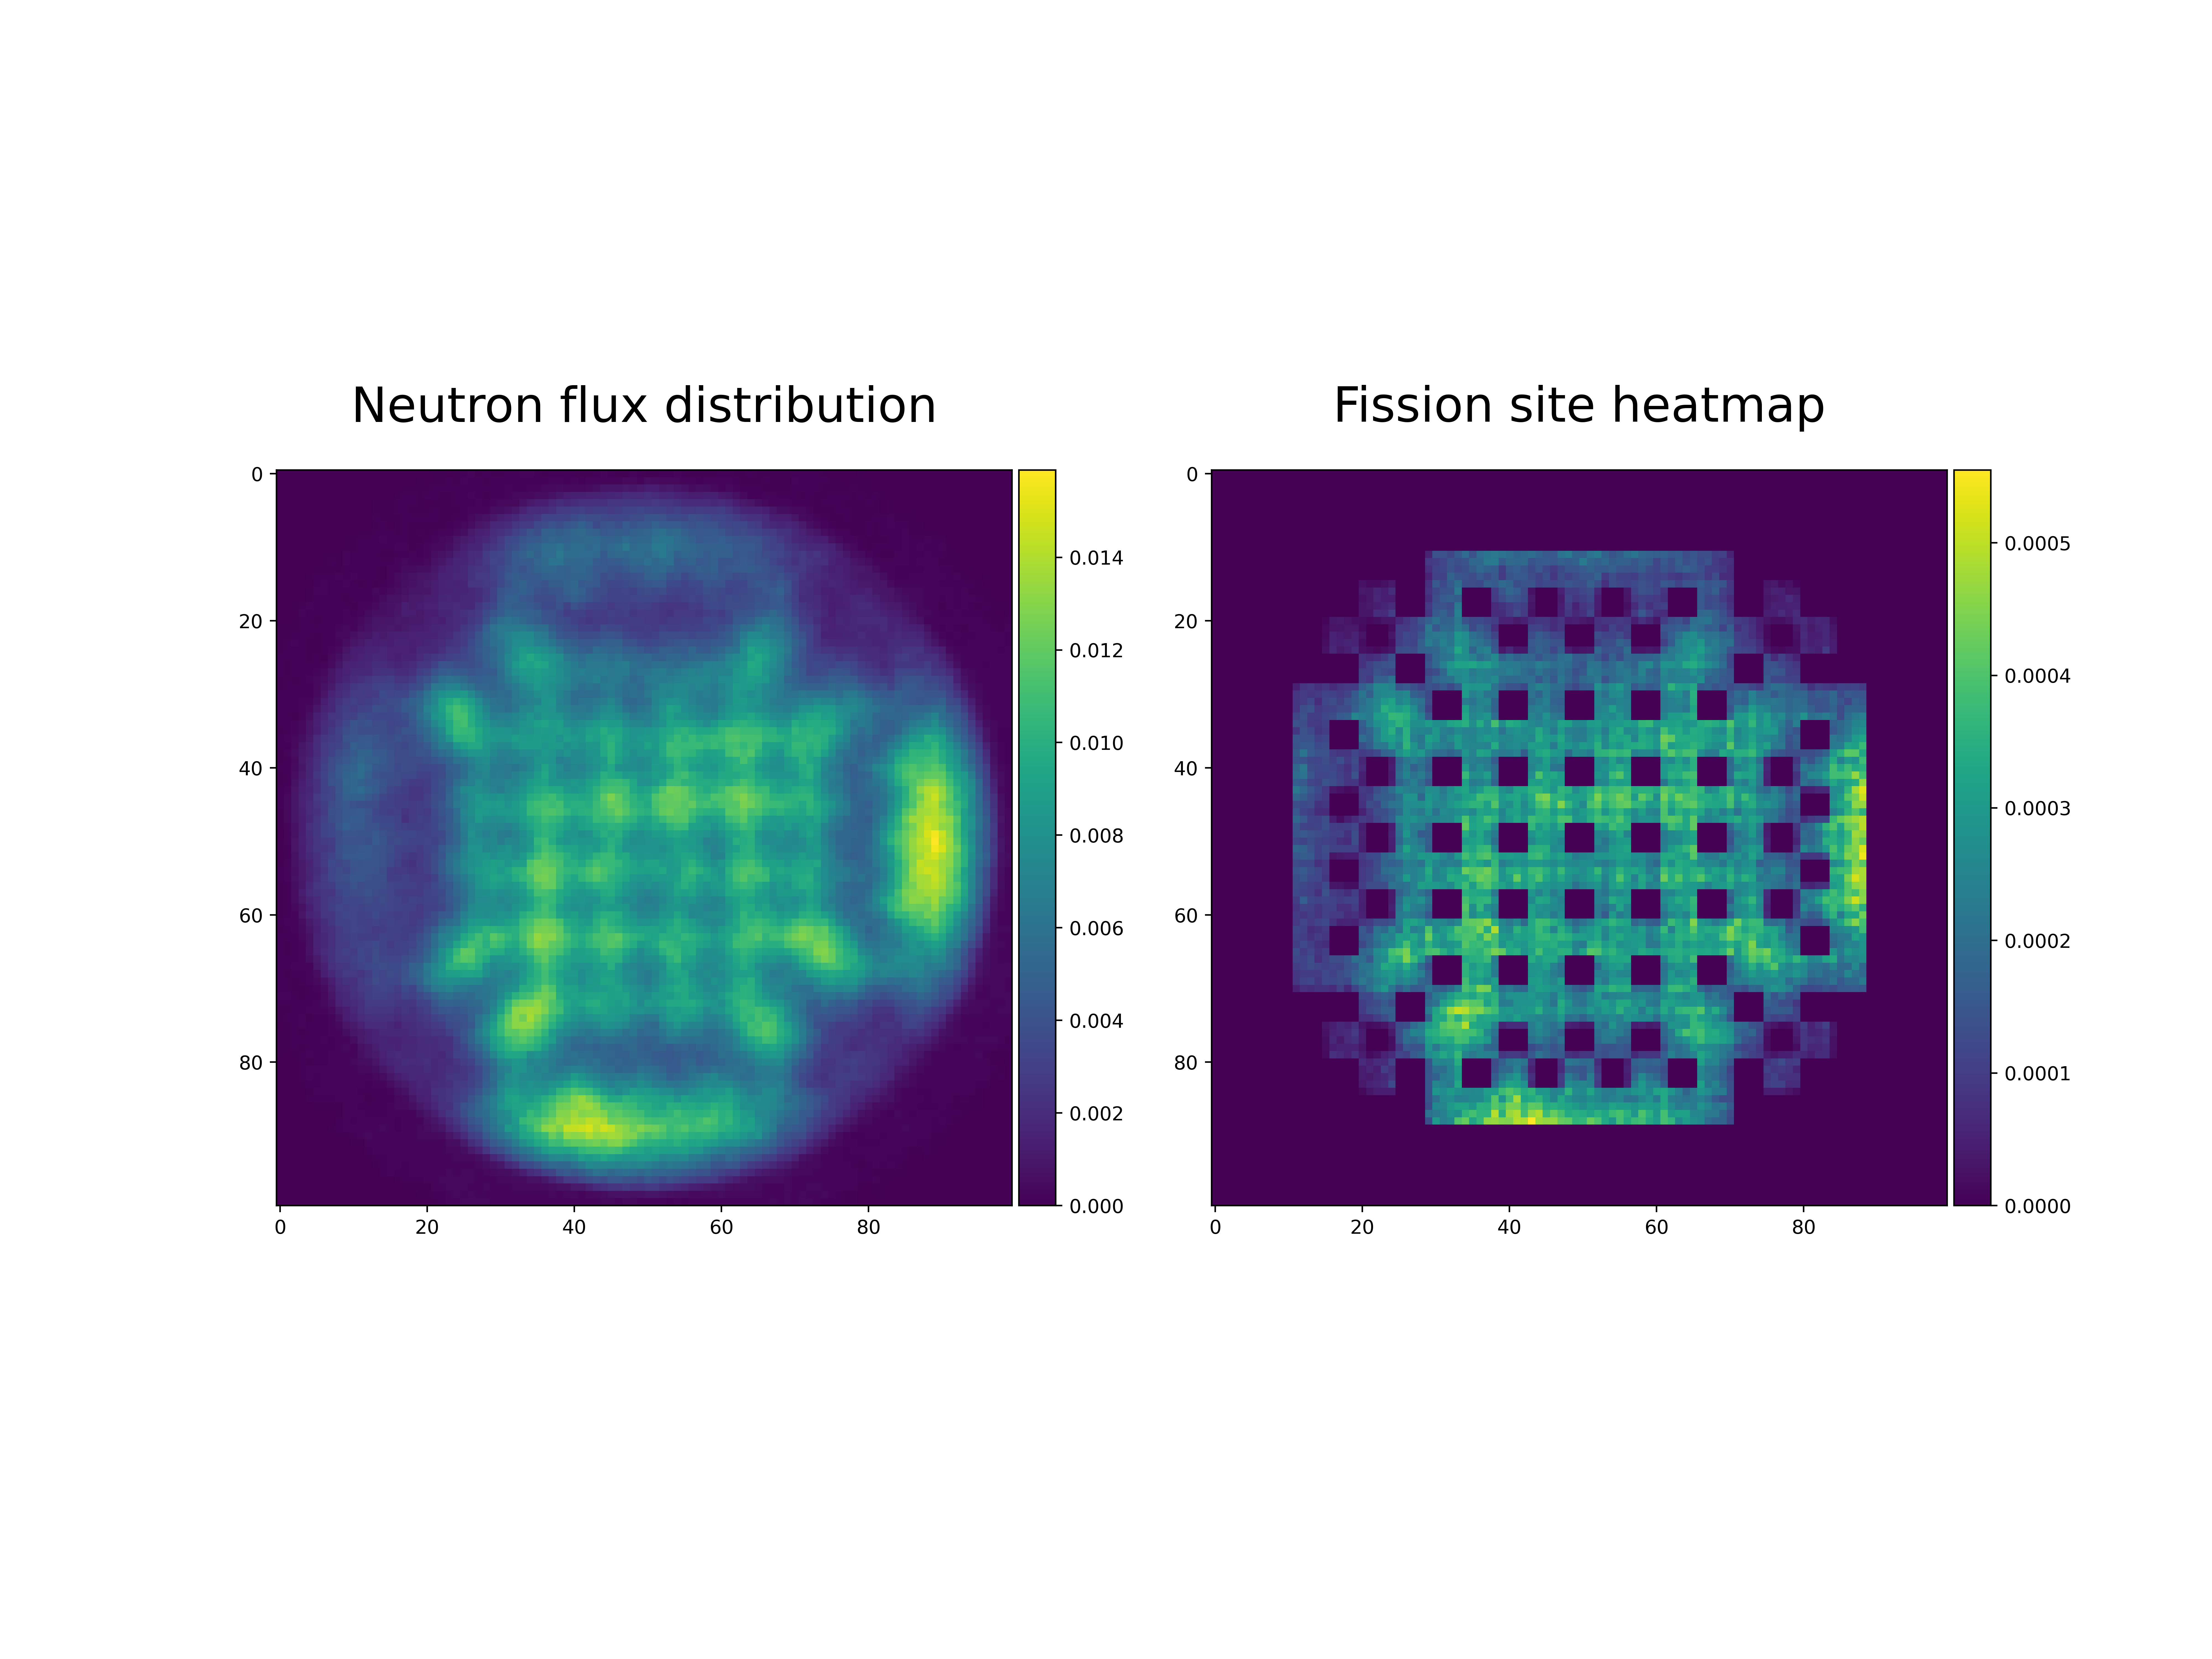
\includegraphics[width=0.4\textwidth]{../Pictures/Mesh_RPV.png}
  \caption{Neutron flux distribution and fission site heatmap for the reactor pressure vessel.}
  \label{fig:meshRPV}
\end{figure}

\par
Sine OpenMc is a Monte Carlo simulation the results are stochastic in nature, this gives a slight different result at every run, so there will always be som statistical fluctuation generated in a plot like the above. Ideally the neutron flux distribution and the fission site heatmap would be more homogeneous. When looking at the plot for the neutron energy distribution in the reactor we obtained the familiar energy distribution with a pean in the thermal region and a peak in fast region, see Fig.~\ref{fig:EnergyRPV}.

% FIGURE: Energy RPV
\begin{figure}[b]
  \centering
  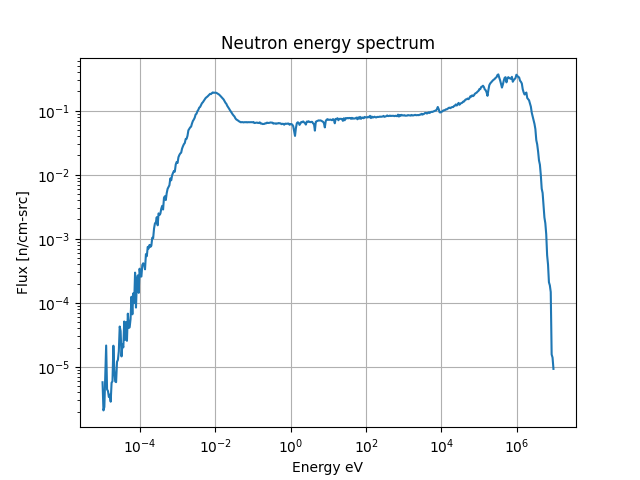
\includegraphics[width=0.4\textwidth]{../Pictures/Energy.png}
  \caption{Neutron energy distribution for the reactor pressure vessel.}
  \label{fig:EnergyRPV}
\end{figure}

\par
Further we investigated one of the most important passive safety mechanisms in a reactor: the Doppler broadening. This effect entails a reduction of the neutron multiplication number as the core/fuel temperature increases due to a higher average kinetic energy of the atoms in the fuel determining a broadening of the resonance absorption region. This means that several neutron get captured by an atom whitout producing any fission. This effect is neatly illustrated in Fig.~\ref{fig:doppler}, where the temperature har been gradually increased by steps of 100 K at a time. For out reactor the optimal operational temperature to achieve criticality was 1474 K for the fuel elements and 902 K for the moderator/coolant. These are also the typical operational temperatures for a commertial PWR.

% FIGURE: Doppler broadening
\begin{figure}[ht]
  \centering
  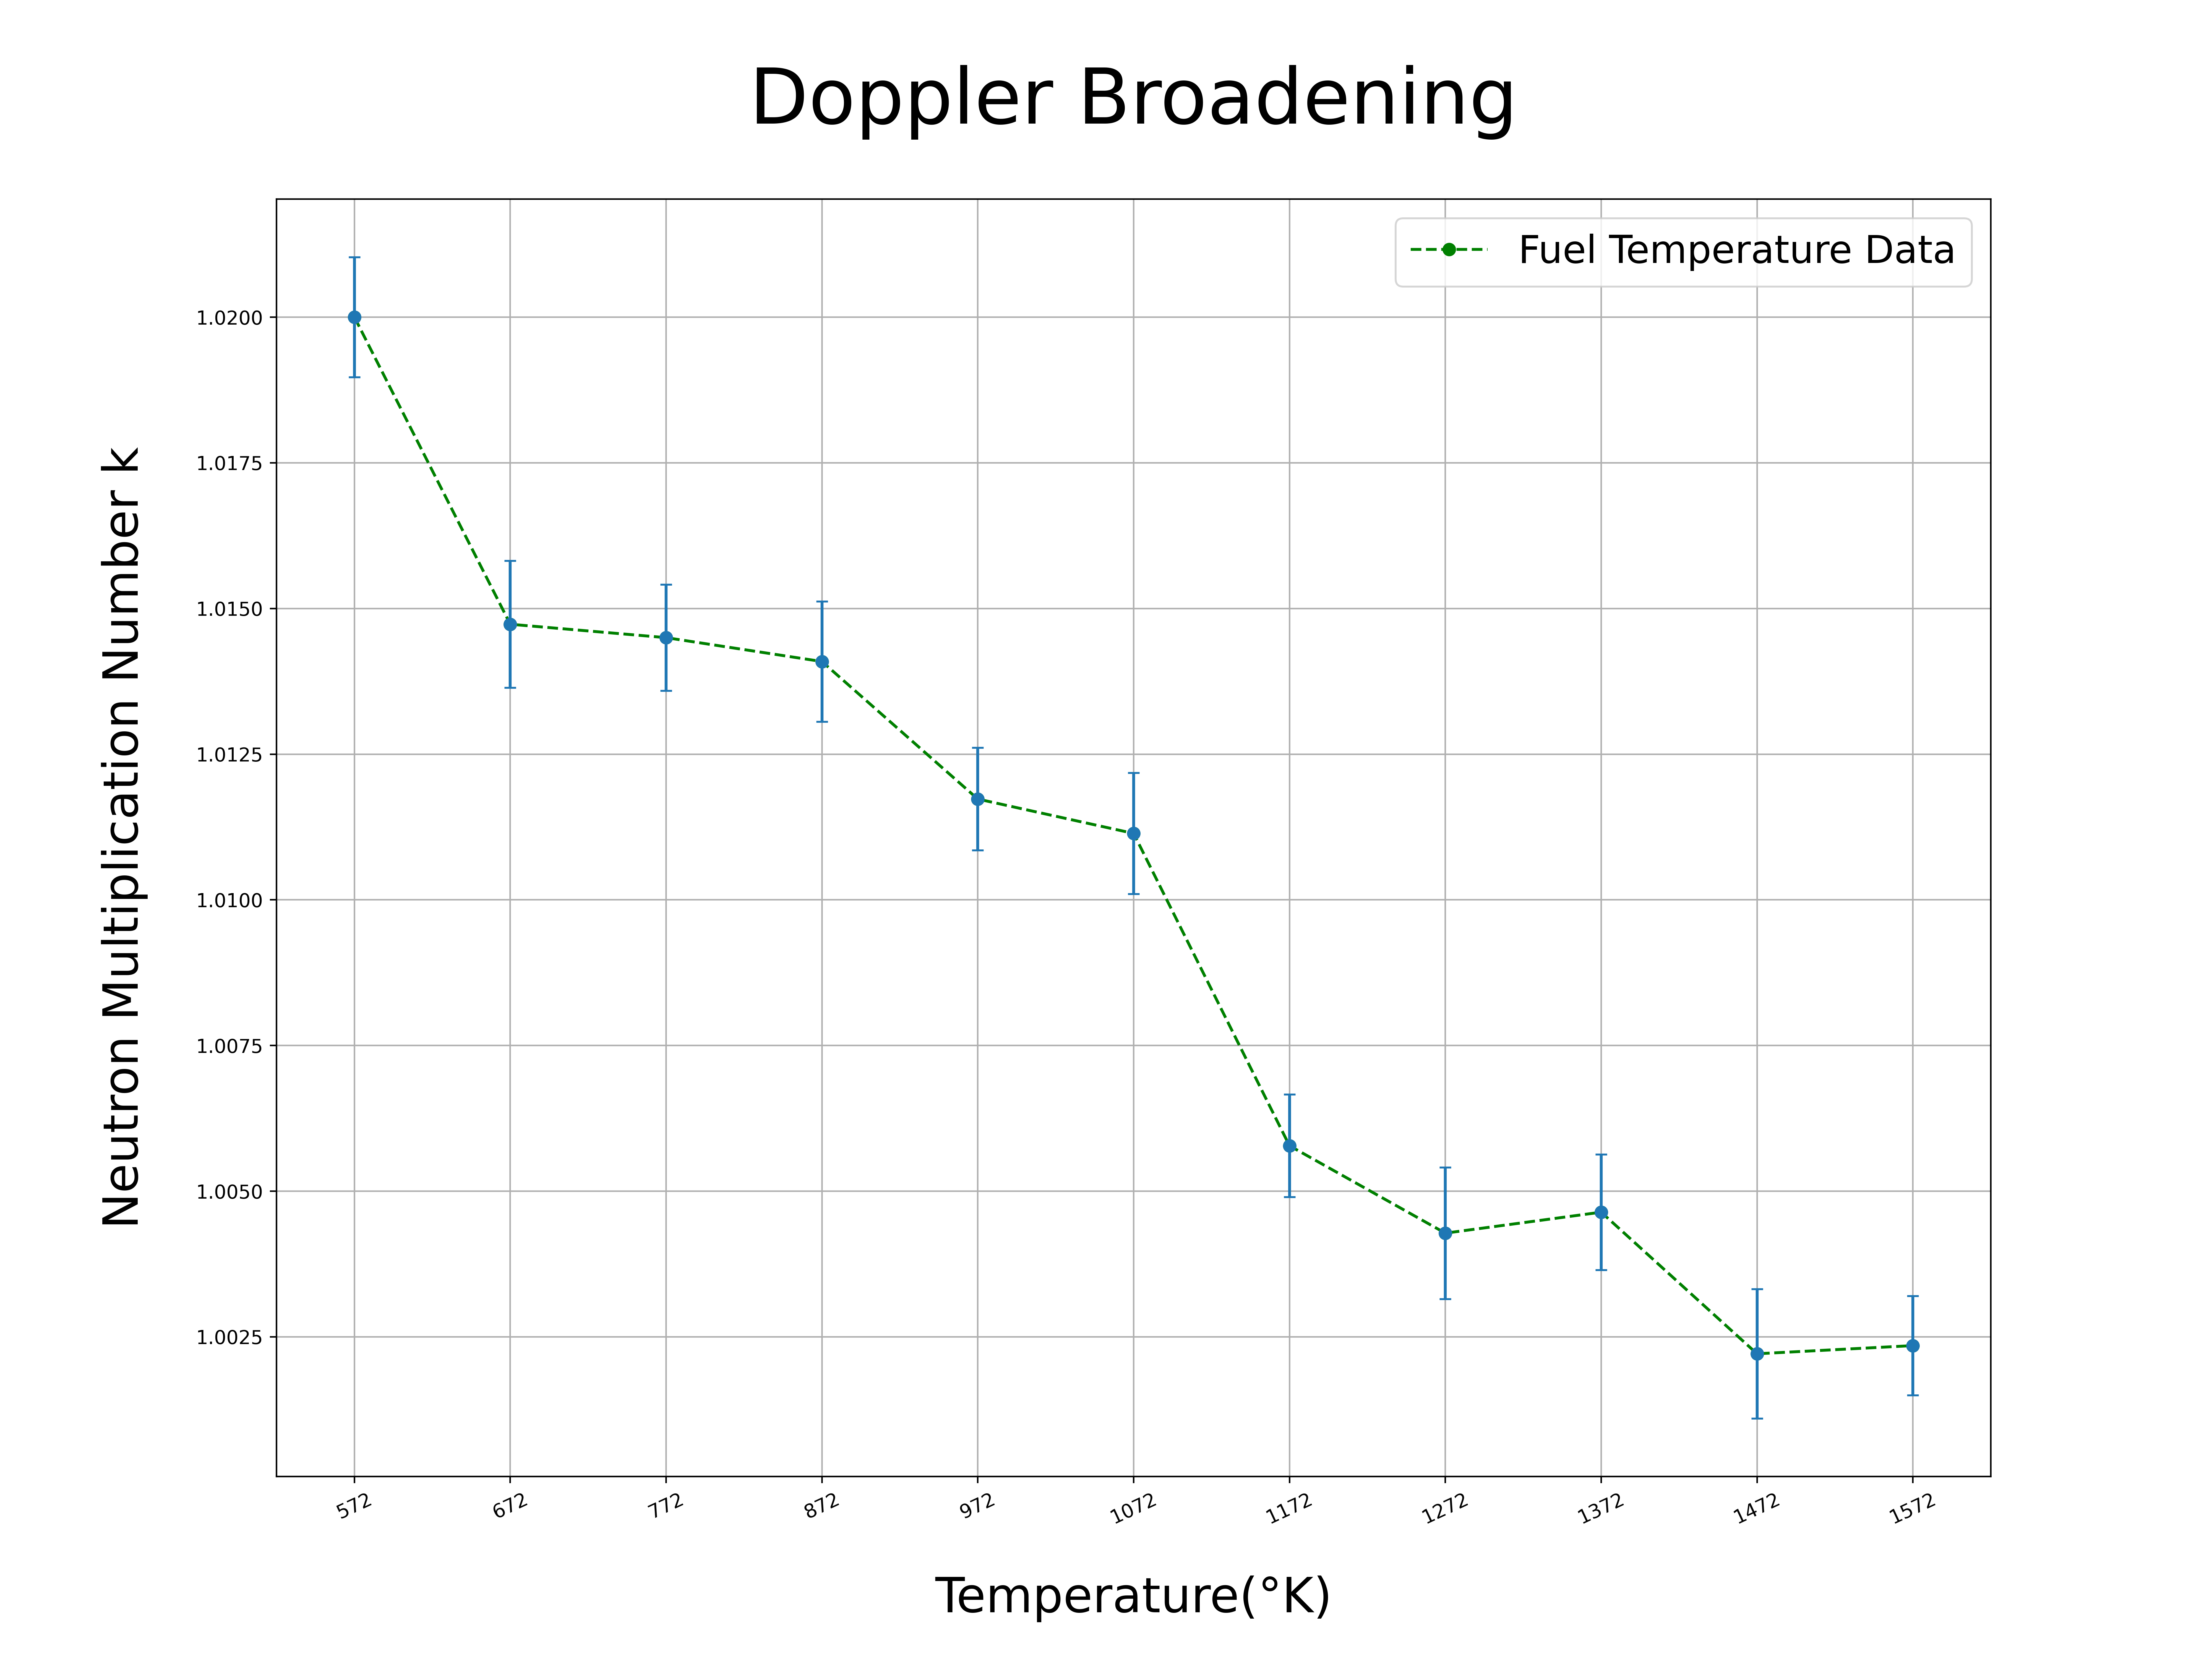
\includegraphics[width=0.4\textwidth]{../Pictures/Doppler.png}
  \caption{Decreasing k-effective as temperature increases due to Doppler broadening.}
  \label{fig:doppler}
\end{figure}

\subsection[Depletion]{\centering Depletion}
\label{subsec:Depletion}

The last step of our project was to study a depletion cycle of our reactor model. A depletion calculation takes into consideration the time development of various elements in a reactor: more specifically the calculation entails the time development of the k-effective value togheter with the various changes in the fuel structure, i.e. its material composition, and the buildup of several fission fragments and neutron poisons. In a typical APWR a fuel cycle lasts 13 months, so we decided to run the the depletion calculation for 56 weeks, one week at a time. The operational power is set at 1200 MW and is held constant throughout the whole fuel cycle. The change in the neutron multiplication number k$_{eff}$ has been illustrated in Fig.~\ref{fig:Depletionkeff}.

% FIGURE: Depletion keff
\begin{figure}[t]
  \centering
  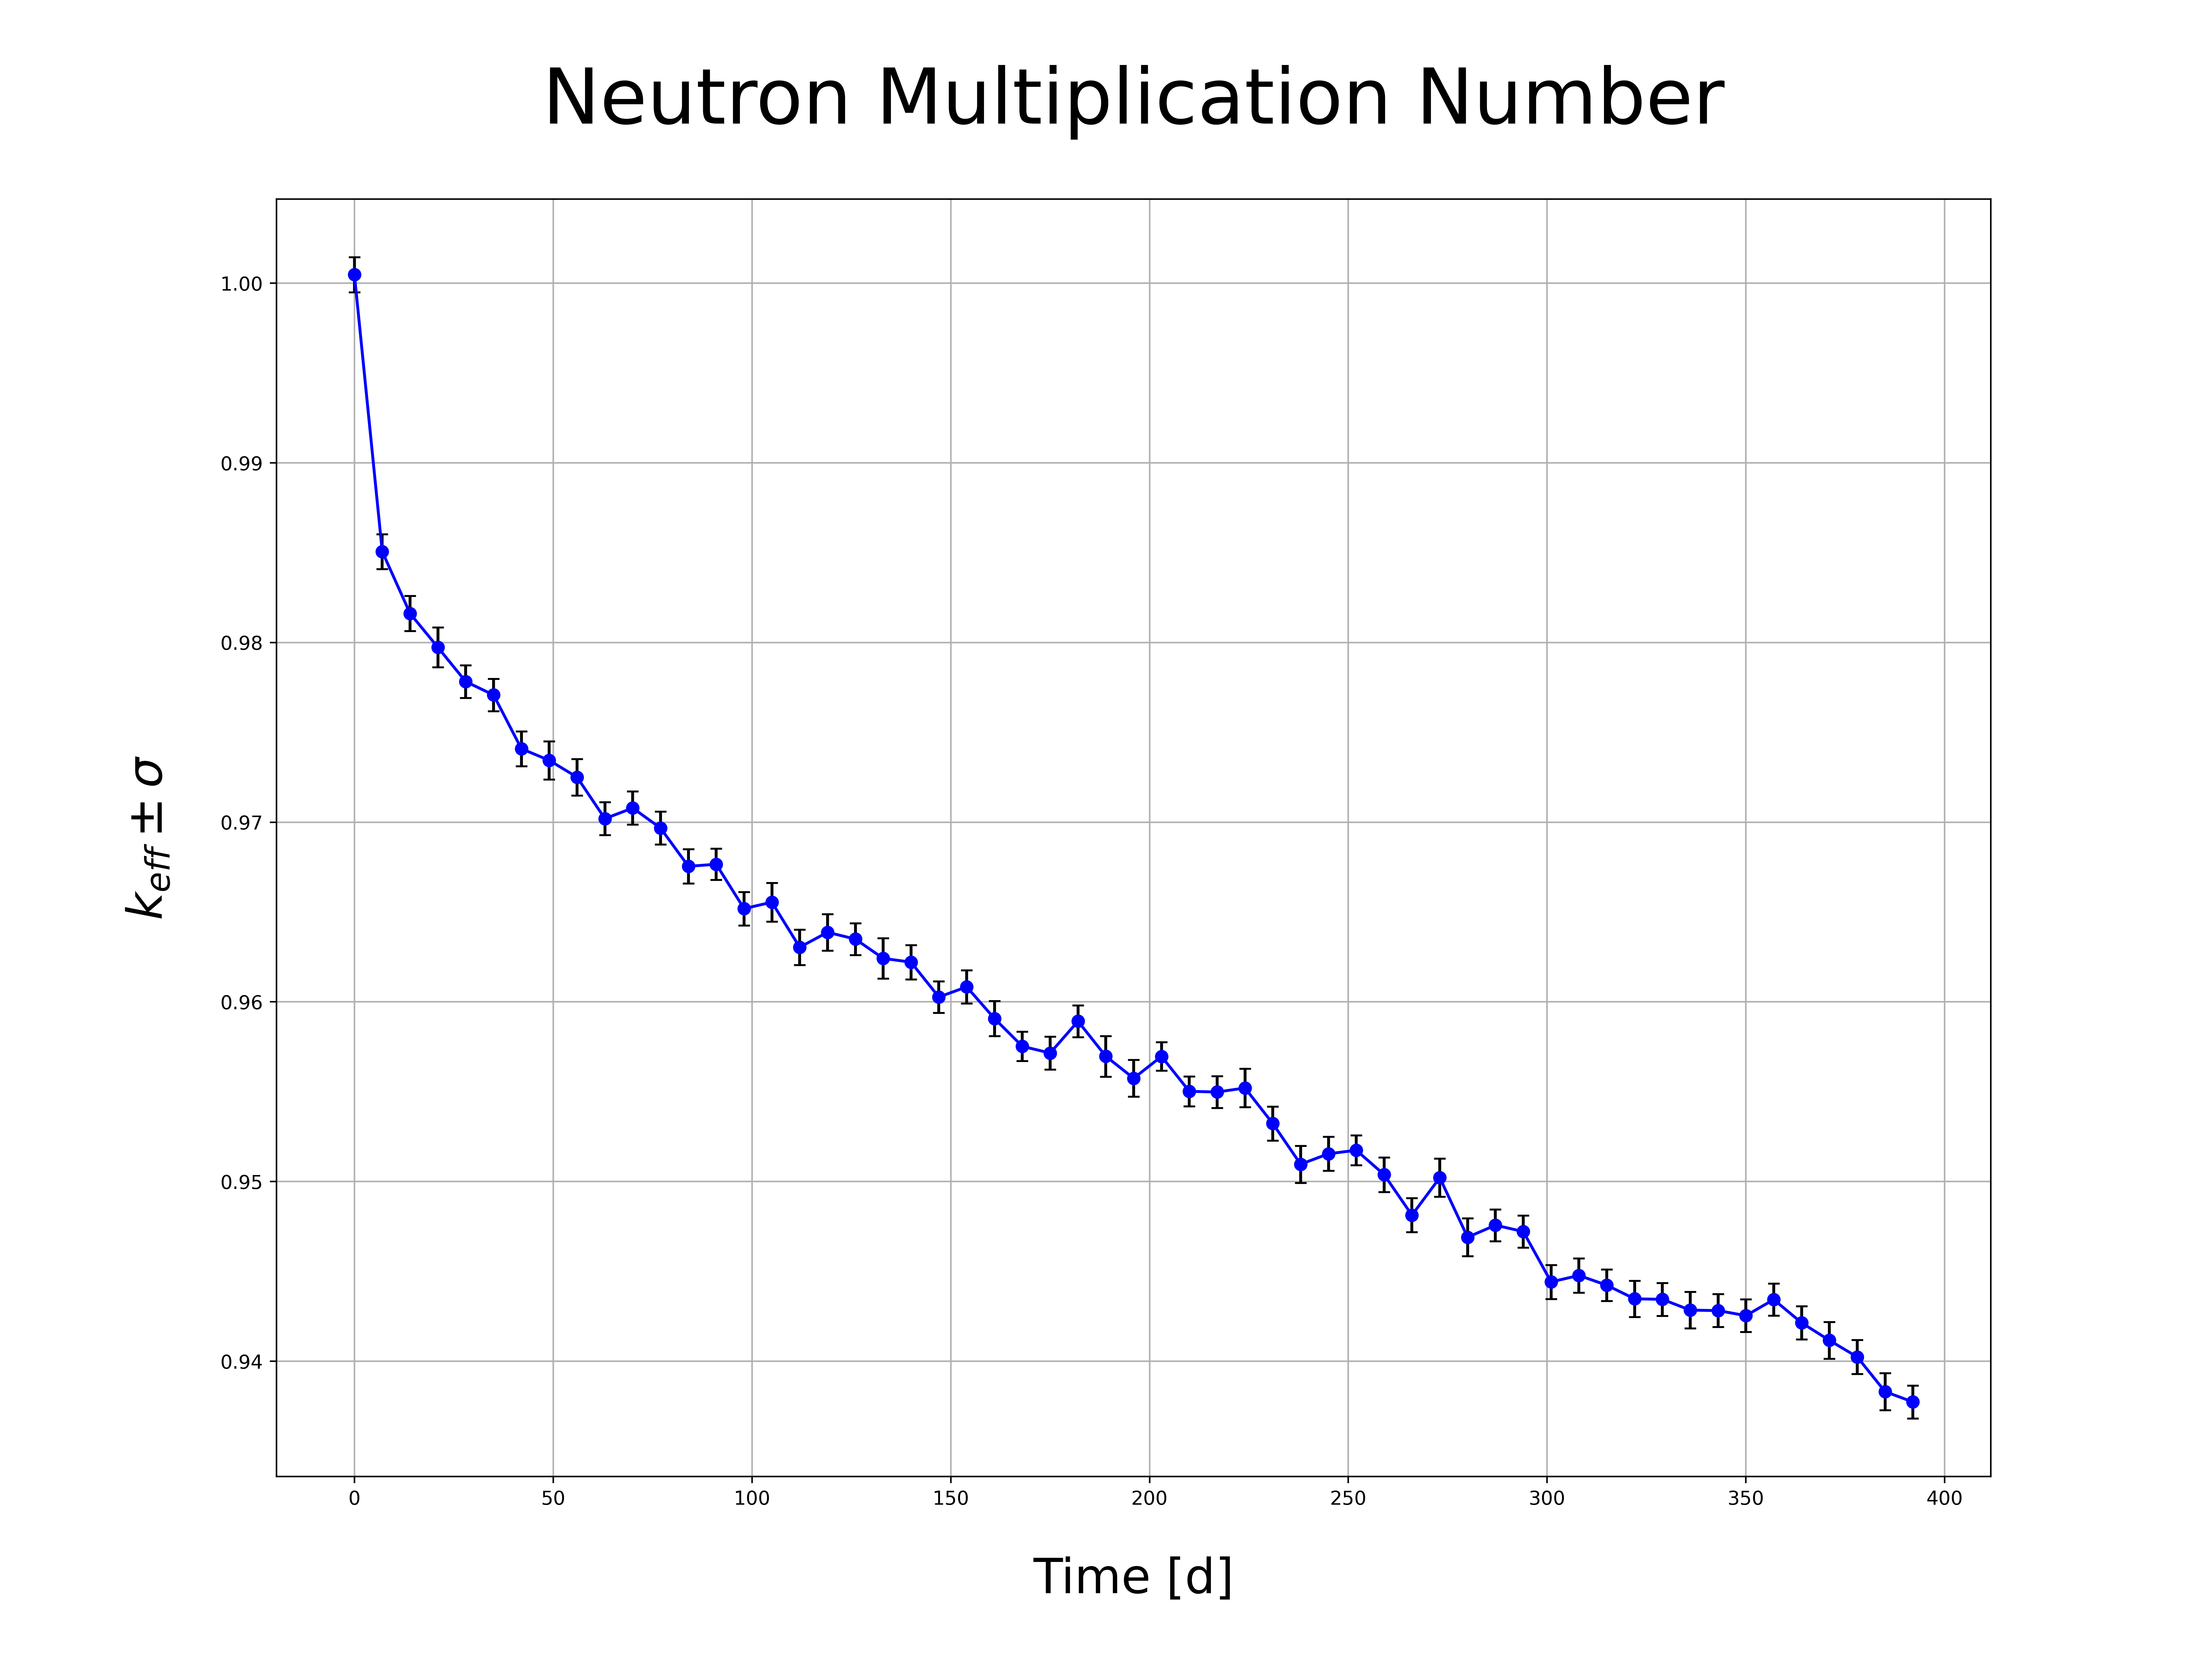
\includegraphics[width=0.4\textwidth]{../Pictures/Depletion_keff.png}
  \caption{Decreasing k-effective as temperature increases due to Doppler broadening.}
  \label{fig:Depletionkeff}
\end{figure}

\par
OpenMc also offers the possibility of checking the fission rate for each single depleted element in addition to its number of atoms. As can be seen in Fig.~\ref{fig:fissionU235}, the fission rate of the fissile U-235 decreases over time; this is due to its constant absorpion of thermal neutron over time, transmutating into U-236 and the fission to two or more lighter fission fragmens. This means that over time the amount of available U-235 will decrease and so will the fission amount caused by this element. The amount of U-235 over the 13-month cycle can be seen in Fig.~\ref{fig:U235vsPu239}.  

% FIGURE: Depletion fission U235
\begin{figure}[ht]
  \centering
  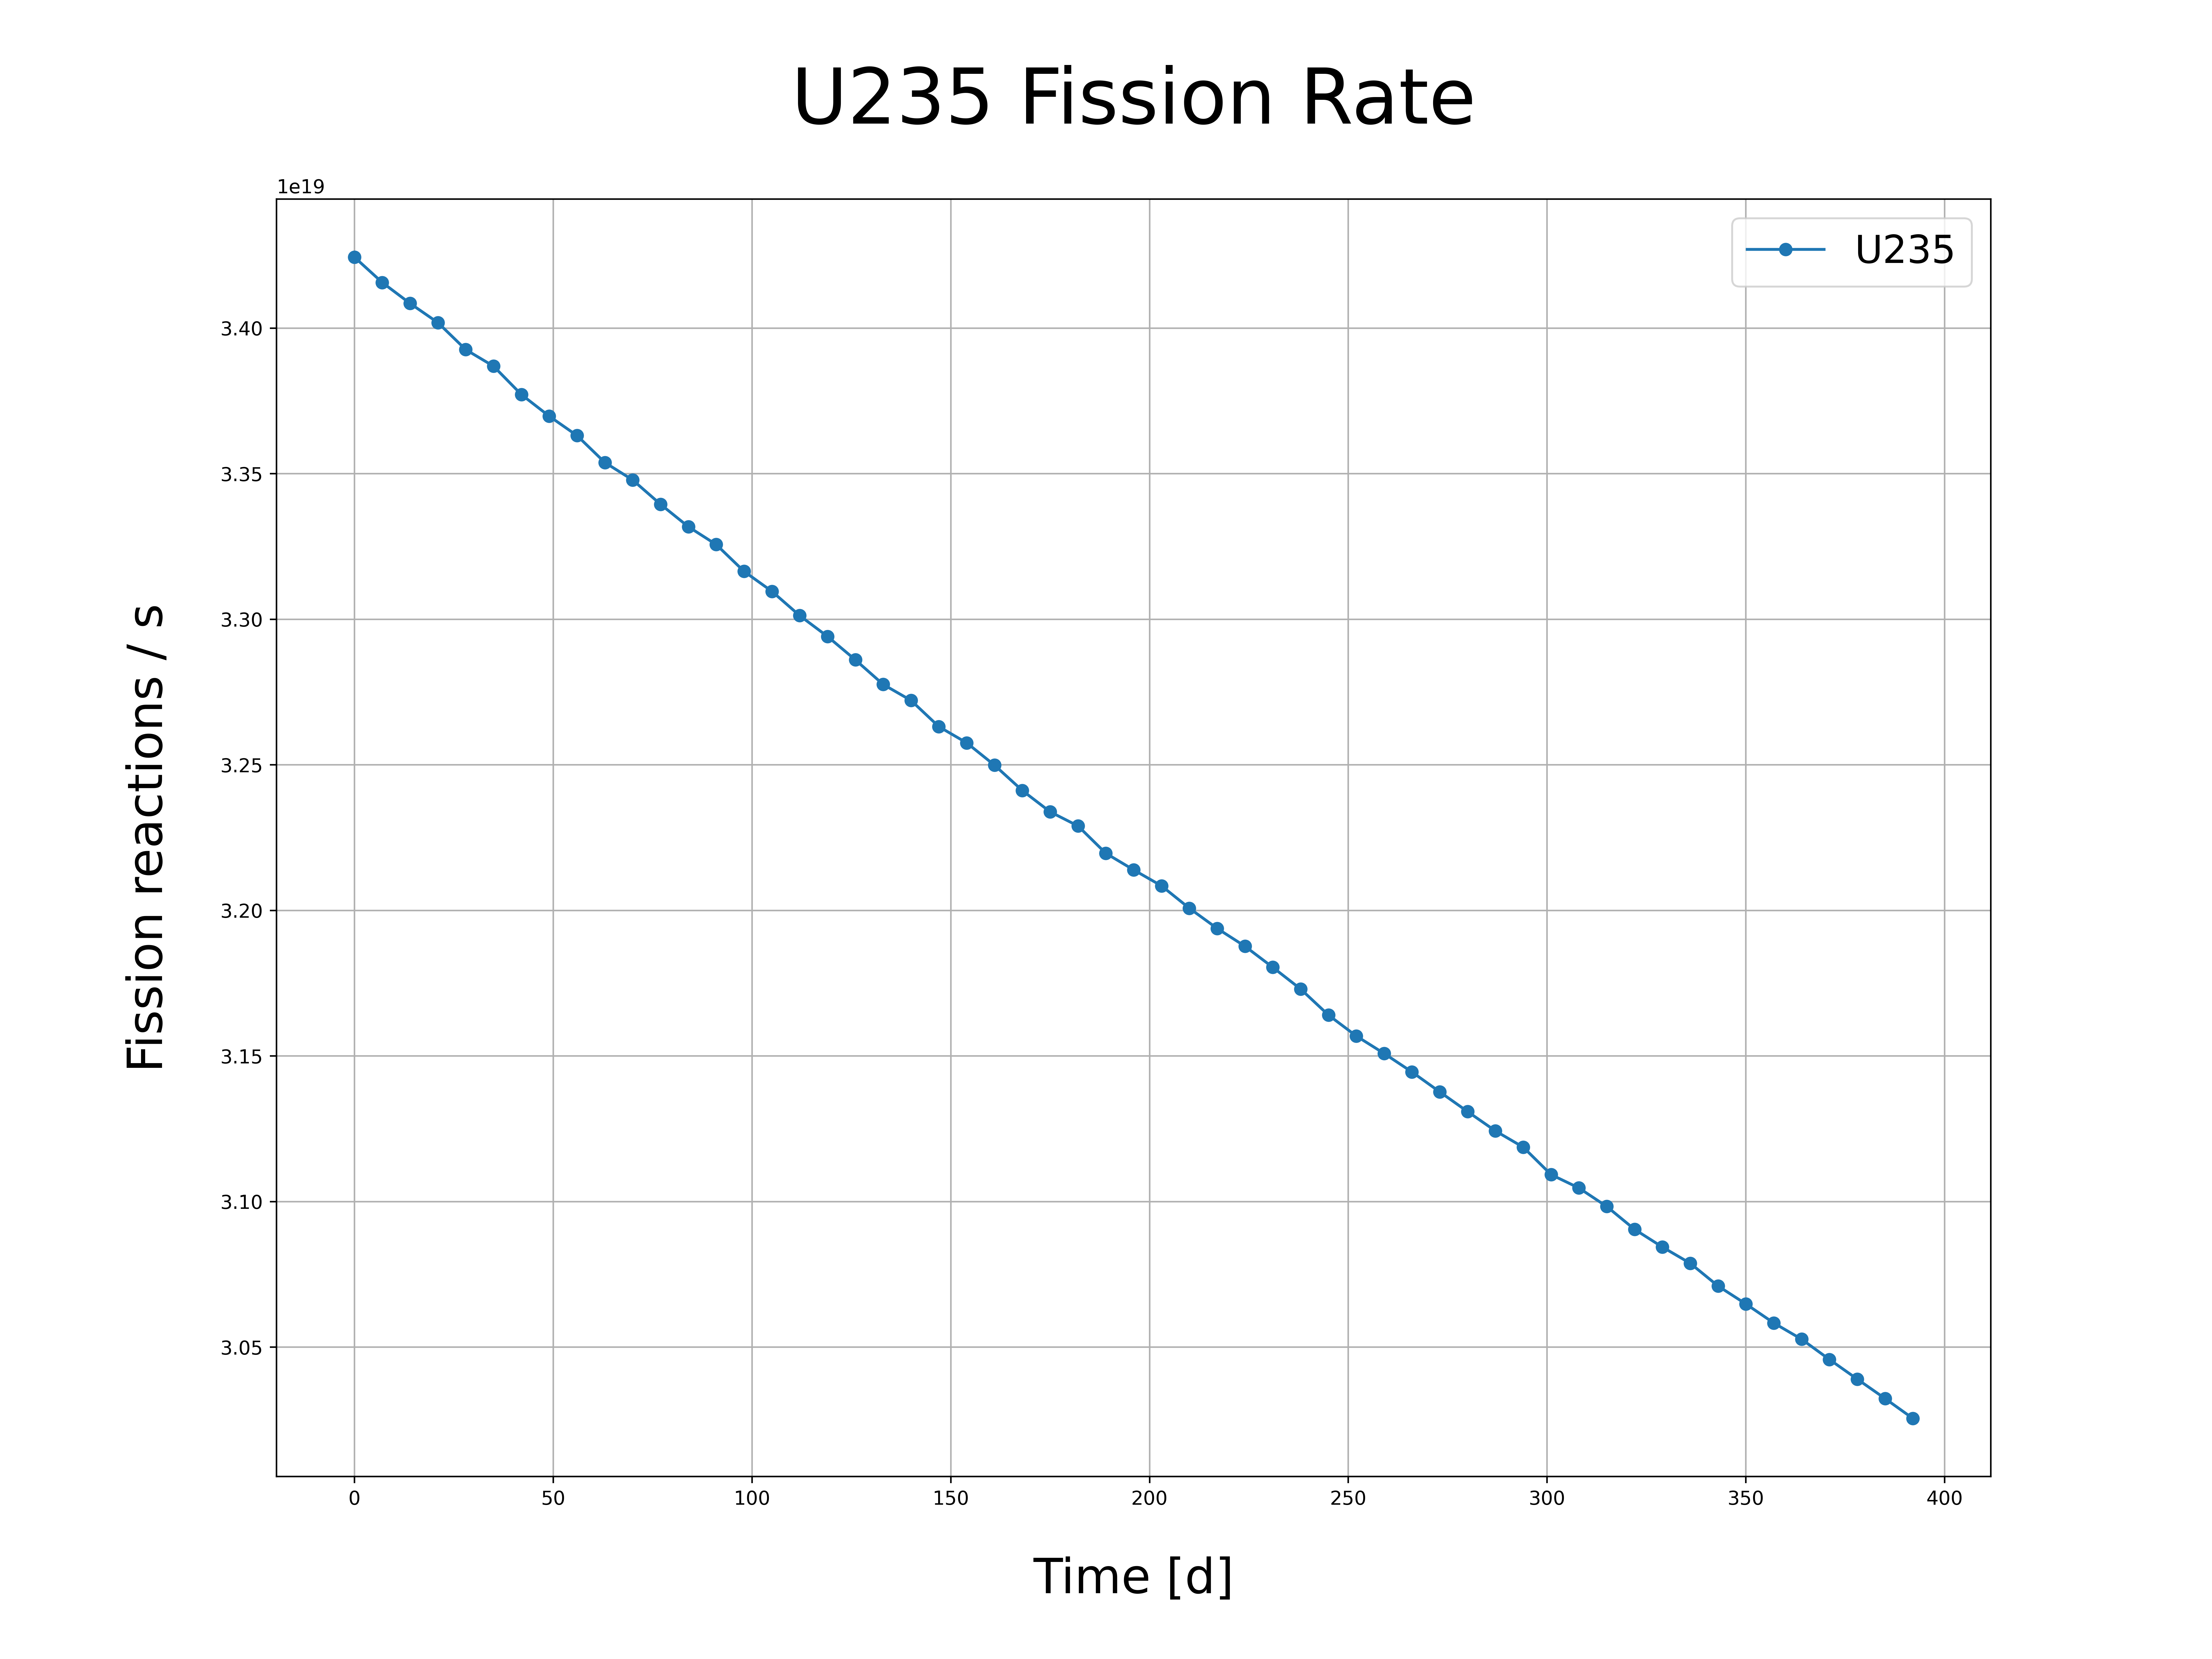
\includegraphics[width=0.4\textwidth]{../Pictures/Depletion_FissionU235.png}
  \caption{Decreasing k-effective as temperature increases due to Doppler broadening.}
  \label{fig:fissionU235}
\end{figure}

% FIGURE: Depletion U235 vs Pu239
\begin{figure}[ht]
  \centering
  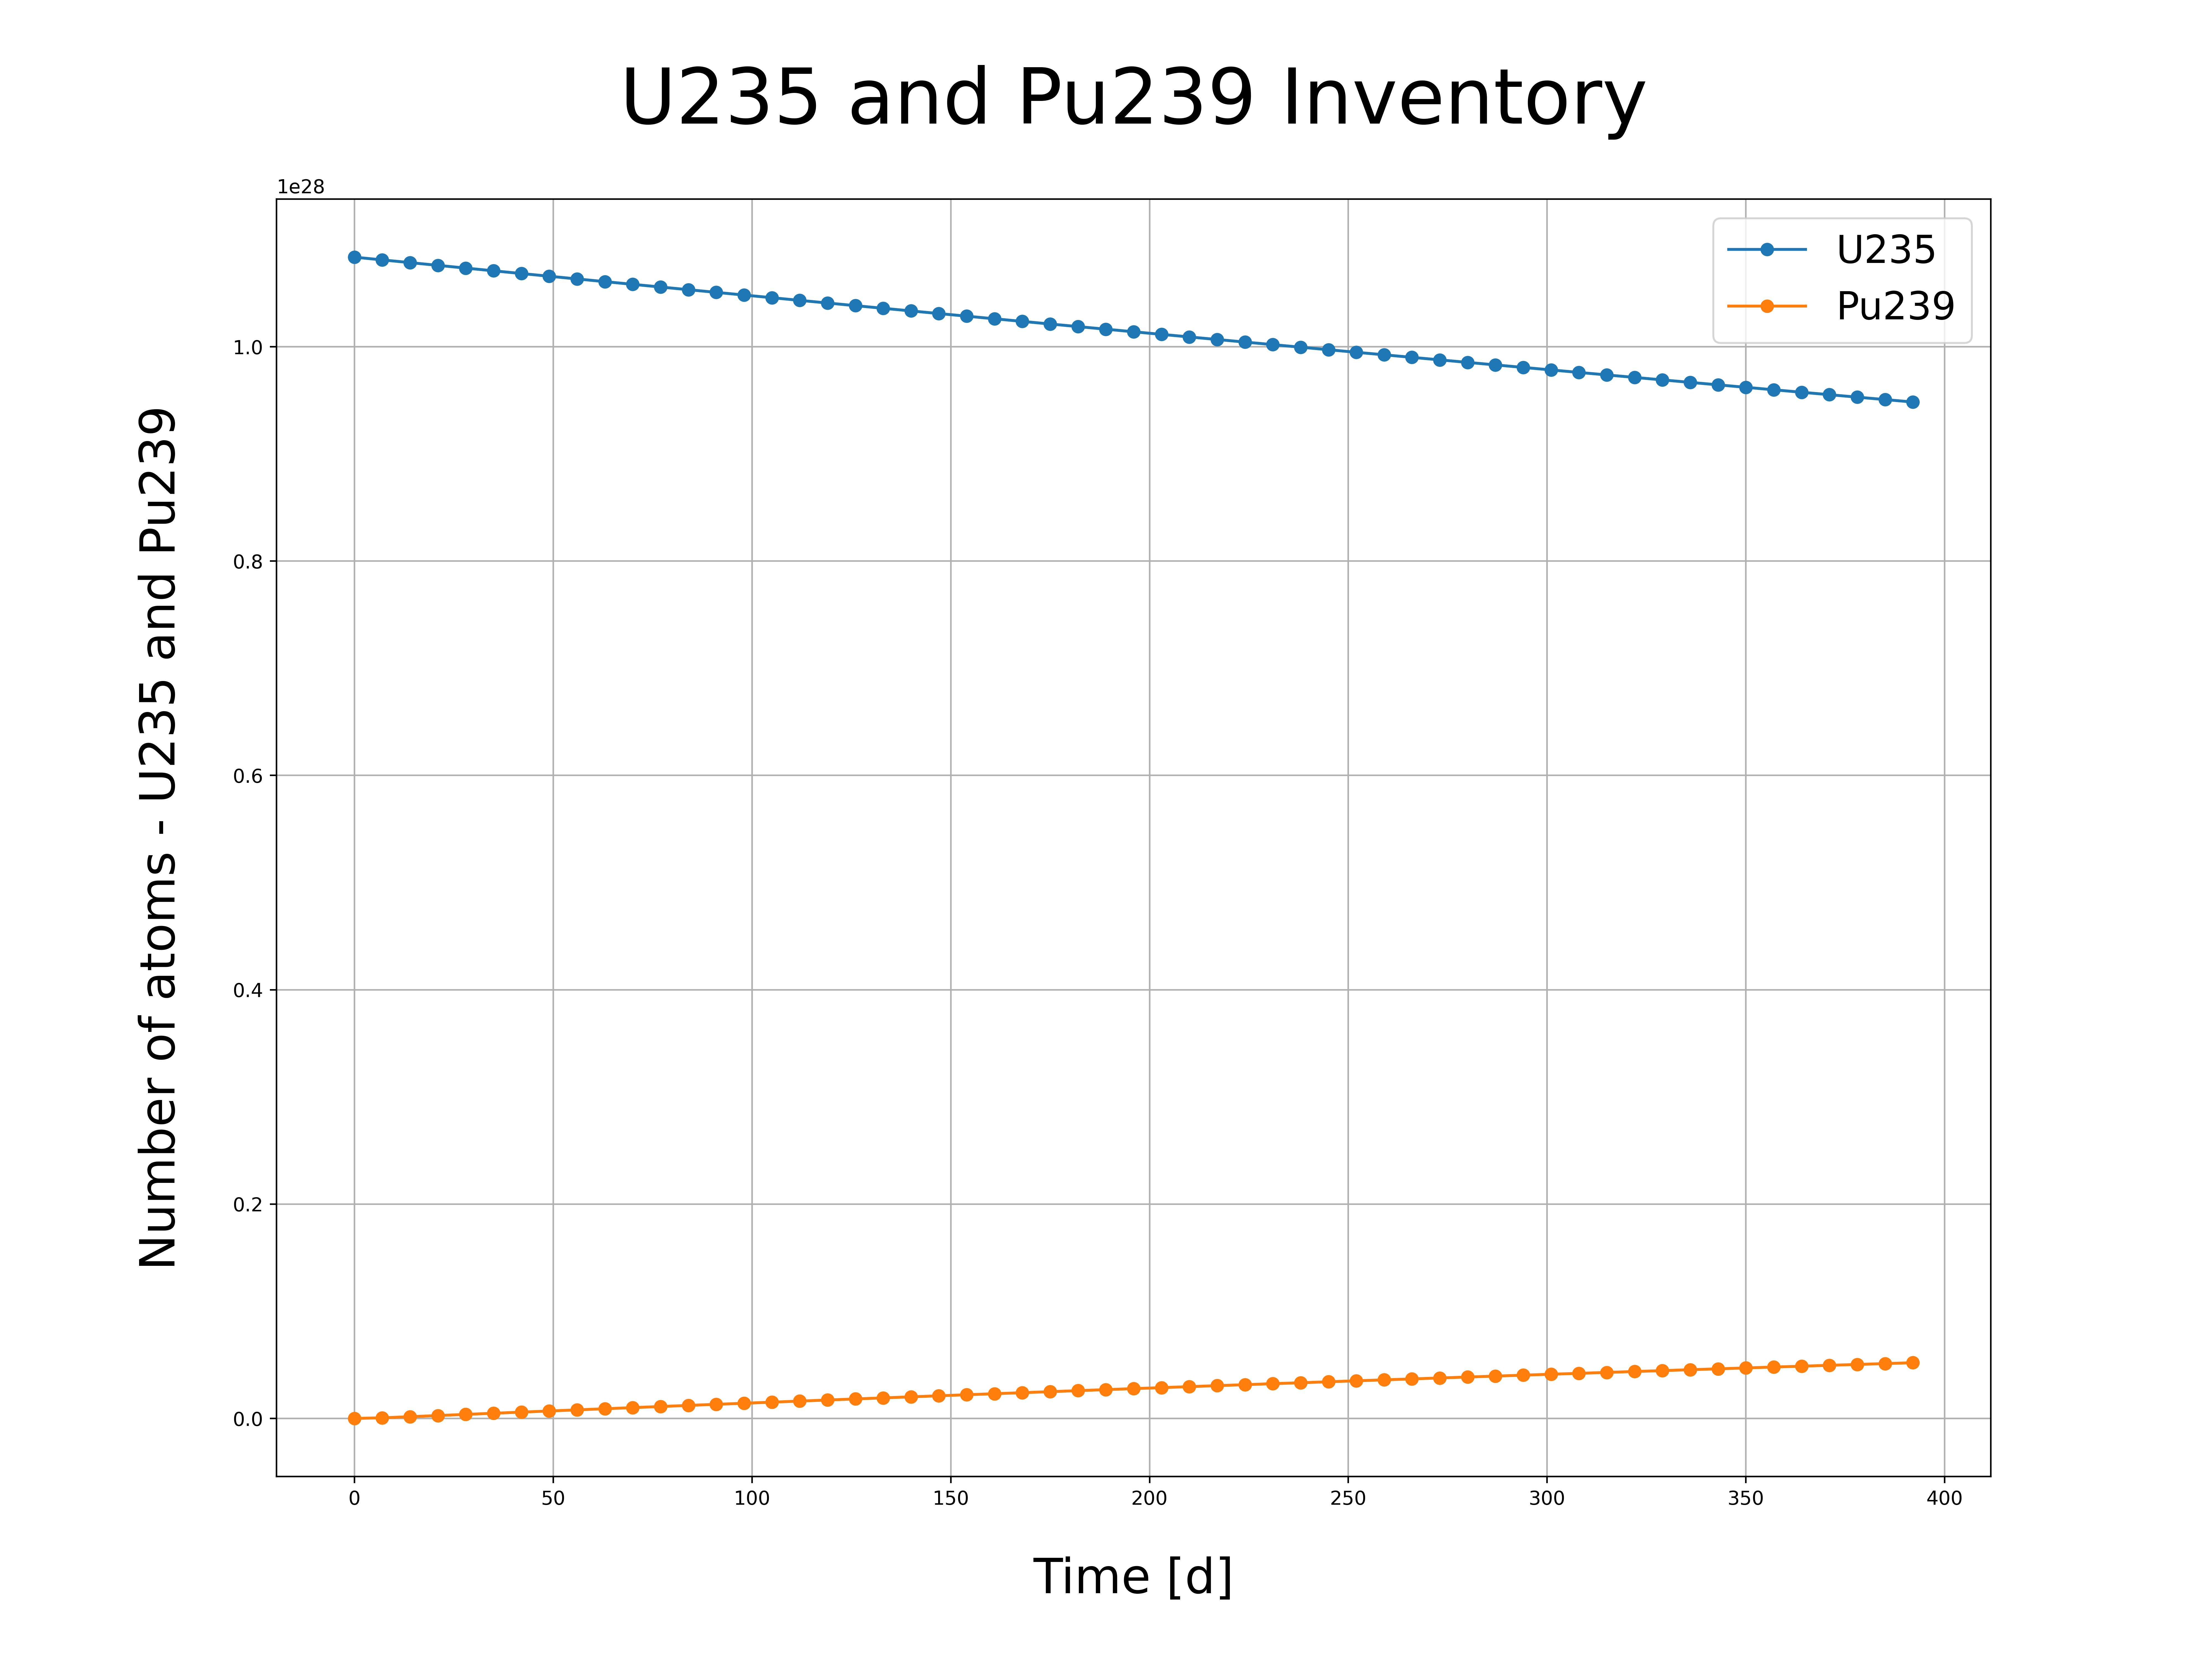
\includegraphics[width=0.4\textwidth]{../Pictures/Depletion_U235_P239.png}
  \caption{Decreasing k-effective as temperature increases due to Doppler broadening.}
  \label{fig:U235vsPu239}
\end{figure}

\par
In addition to U-235 transmutation and subsequent fission another nuclear reaction of notice is taking place inside the reactor core: the transmutation of fertile U-238 into fissile Pu-239. This means that U-238 absorbs a neutron and becomes U-239, which in turn beta-deacys to Np-239 that will in turn beta-deay to Pu-235. This means that the U-238 quantity is reduced over time while the Pu-239 quantity increases accordingly. It follows that this kind of reactor breed Pu-239 that in the worst case scenario could be used to craft a nuclear bomb.

% FIGURE: Depletion Xe135 and Sm149
\begin{figure}[ht]
  \centering
  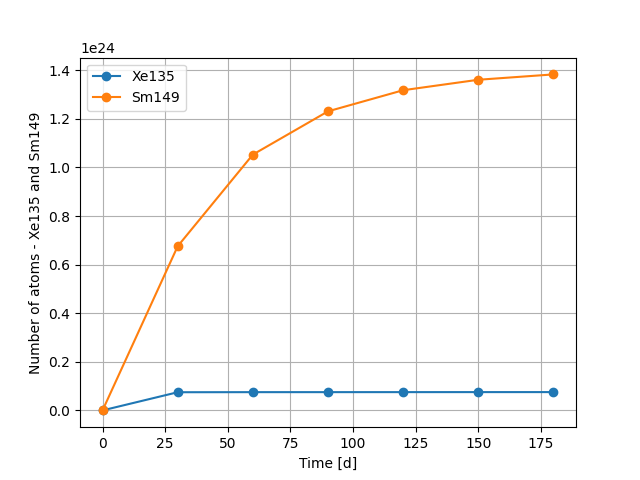
\includegraphics[width=0.4\textwidth]{../Pictures/Depletion_Xe135_Sm149.png}
  \caption{Decreasing k-effective as temperature increases due to Doppler broadening.}
  \label{fig:Xe135andSm149}
\end{figure}

\par
Lastly some of the fission fragments that build up in the reactor are neutron poisons, i.e. they absorb neutrons without yielding any new nuclear fission. To of the most important poisons to remeber in a reactor simulation are Xe-135 and Sm-149, since they influence the timing of the reacotr shutdown and restart especially when refueling. These are illustrated in Fig.~\ref{fig:Xe135andSm149}, and follow the theoretical prediction for these elements.

%####################################################################################################################################################
% 3 - RESULTS AND DISCUSSION
%####################################################################################################################################################

\section{Results and Discussion}
\label{sec:Results and Discussion}

In conclusion we can say that our reactor model behaves in a physically acceptable manner eventhoug some consideration about its validity are in order. Due to the limited computing capability of modern computers the particle number in our reactor is quite limited and several orders of magnitude smaller then in a real reactor. Many passive and active safety mechanisms have not been implemented and the reactor pressure vessel is missing the top and bottom part. In addittion the pressurised water as our moderator/coolant is static aand there is no fluid flow through the reactor. Troughout the depletion process it was not possible to adjust the control rods' insertion nor the concentration of boric acid and other neutron poison in the moderator. The power was kept constant, something that usually is not the case in an operational reactor. Factors like decay heat, fission of other elements than U-235 has not been implemented and control of beta-delayed neutrons has been ignored. So in conclusion the obtained value for the neutron multiplication number needs several adjustments and would ideally be kept constant during the reactor operation time. Lastly fuel rotation has not been implemented and this would have a great effect on the measured/real criticality. 

%####################################################################################################################################################
% 4 - CONCLUSION AND FURTHER DEVELOPMENTS
%####################################################################################################################################################

\section[Conclusion and Further Developments]{Conclusion and \newline Further Developments}
\label{sec:Conclusion}

In this project report we have presented a simplified model of an advanced pressurized water reactor, going through its design features from pin cells to reactor pressure vessel. The proposed APWR differs from a regular PWR in size, it is desinged to be bigger, and contains on average more fuel rods. In addition the fuel assembly design includes a higher gadolinium enrichment and a peculiar control rod design. The expected power output of an APWR is higher than a regular PWR and its fuel cycle is longer \cite{APWR}. Some further developments include taking into account the topics discussed in the previous section in addition to fixing some of the problems in the definition of tallies for the factors in the five-factor formula, which have been taken from the OpenMc documentation \cite{DocumentationPinCell,DocumentationDepletion}. 

\vfill\null
\newpage

%####################################################################################################################################################
% REFERENCES
%####################################################################################################################################################

\small
\bibliography{Project}{}
\bibliographystyle{JHEP}
\begin{thebibliography}{}

\bibitem{APWR}
K.~Seki, T.~Tanaka, Y.~Matsuura, \textit{Core and Fuel Design of APWR}, (GENES4/ANP2003,
Paper 1099,  International conference on global environment and advanced nuclear power plants, (p. 1675). Japan: Atomic Energy Society of Japan, Sep. 15-19, 2003,\\ Kyoto, JAPAN. IAEA INIS)
\url{https://inis.iaea.org/search/searchsinglerecord.aspx?recordsFor=SingleRecord&RN=36011909}

\bibitem{DocumentationPinCell}
OpenMC documentation on ``\textit{Tally Arithmetics}":\\
\url{https://docs.openmc.org/en/v0.11.0/examples/tally-arithmetic.html}

\bibitem{DocumentationDepletion}
OpenMC documentation on ``\textit{Pin Cell Depletion}":\\
\url{https://docs.openmc.org/en/v0.12.2/examples/pincell_depletion.html}

\bibitem{BurnupFuel}
K. Hesketh, \textit{Material Properties/Oxide Fuels for Light Water Reactors and Fast Neutron Reactors}, Comprehensive Nuclear Materials (2012)\\
\url{https://www.sciencedirect.com/topics/earth-and-planetary-sciences/gadolinium}

\bibitem{GitHub}
Author's GitHub repository for OpenMc simulation source code:\\
\url{https://github.com/KevinCappa/FYS4580_Project.git}

\end{thebibliography}
\vfill\null
\newpage

%####################################################################################################################################################
% APPENDIX
%####################################################################################################################################################

\twocolumn[
\begin{@twocolumnfalse}
\appendix
\section*{\centering Appendix: Figures and Plots \\ \noindent\rule[5pt]{8cm}{0.4pt} \\}
\end{@twocolumnfalse}
]

\begin{figure}[t]
  \centering
  \includegraphics[width=0.3\textwidth]{../Pictures/Burnablefuelrods_plot_xy.png}
  \caption{Top view of the burnable fuel pin cell.}
  \label{fig:burnfuel_xy}
\end{figure}

\begin{figure}[ht]
  \centering
  \includegraphics[width=0.3\textwidth]{../Pictures/Burnablefuelrods_plot_yz.png}
  \caption{Side view of the burnable fuel pin cell.}
  \label{fig:burnfuel_yz}
\end{figure}

\begin{figure}[b]
  \centering
  \includegraphics[width=0.3\textwidth]{../Pictures/Controlrods_plot_xy.png}
  \caption{Side view of the control pin cell.}
  \label{fig:controlpin_xy}
\end{figure}

\begin{figure}[t]
  \centering
  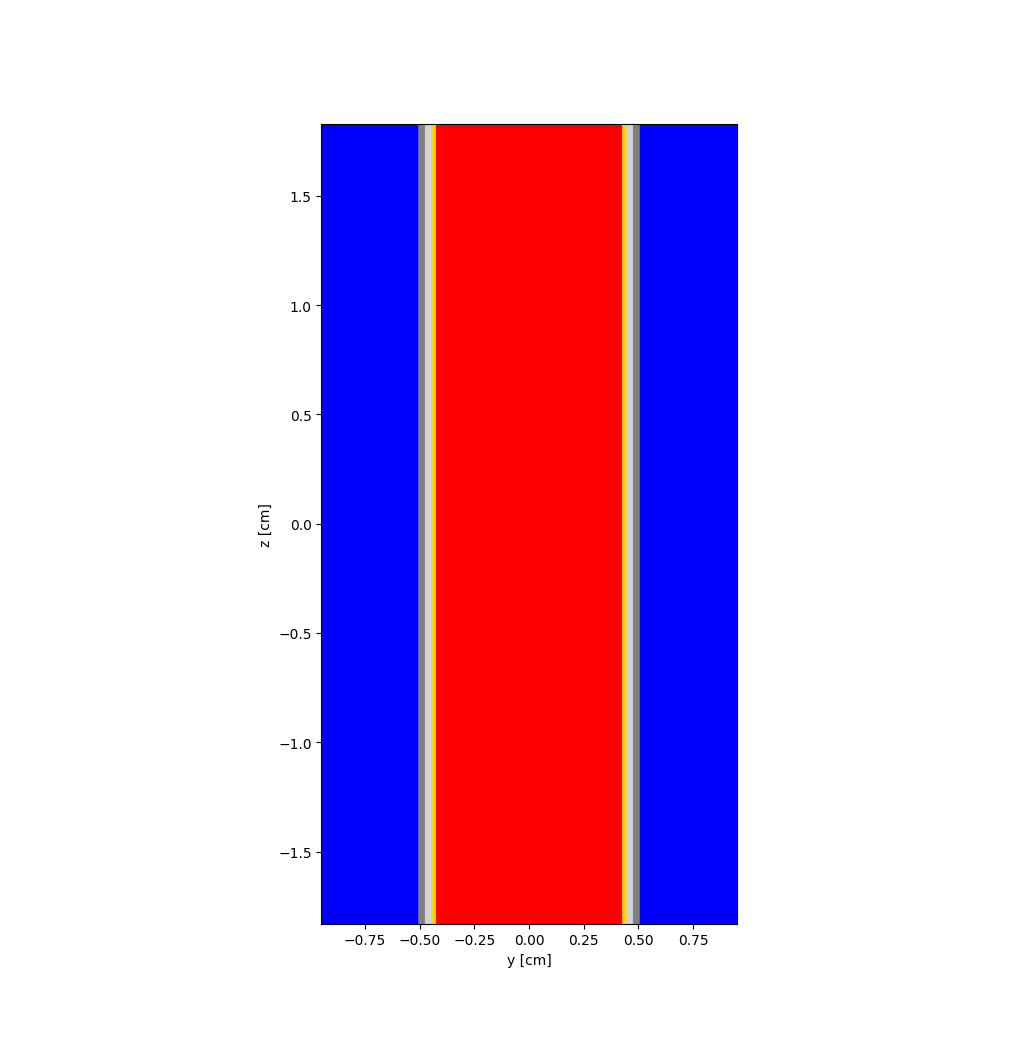
\includegraphics[width=0.3\textwidth]{../Pictures/Controlrods_plot_yz.png}
  \caption{Side view of the control pin cell.}
  \label{fig:controlpin_yz}
\end{figure}

\begin{figure}[ht]
  \centering
  \includegraphics[width=0.3\textwidth]{../Pictures/Thimbleguides_plot_xy.png}
  \caption{Side view of the guide thimble pin cell.}
  \label{fig:guidepin_xy}
\end{figure}

\begin{figure}[ht!]
  \centering
  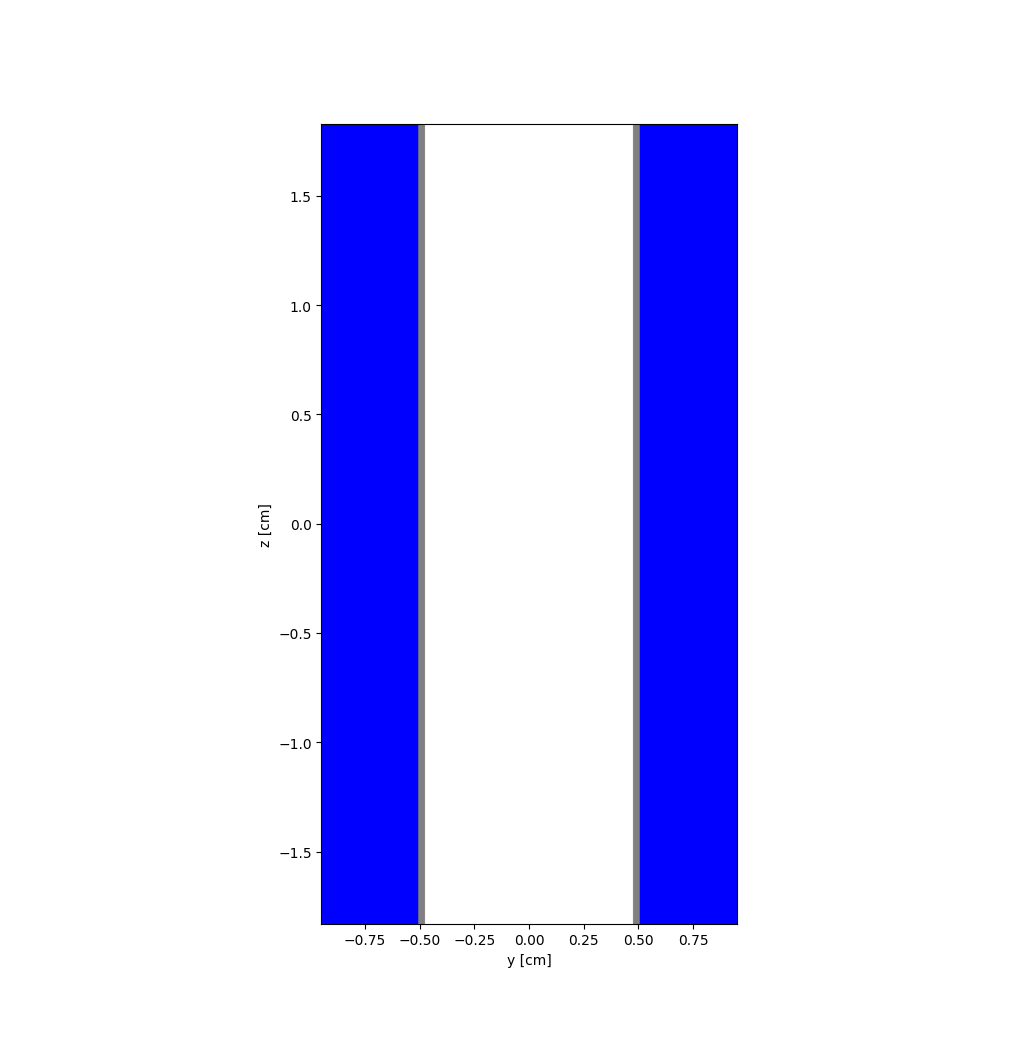
\includegraphics[width=0.3\textwidth]{../Pictures/Thimbleguides_plot_yz.png}
  \caption{Side view of the guide thimble pin cell.}
  \label{fig:guidepin_yz}
\end{figure}

\begin{figure}[ht]
  \centering
  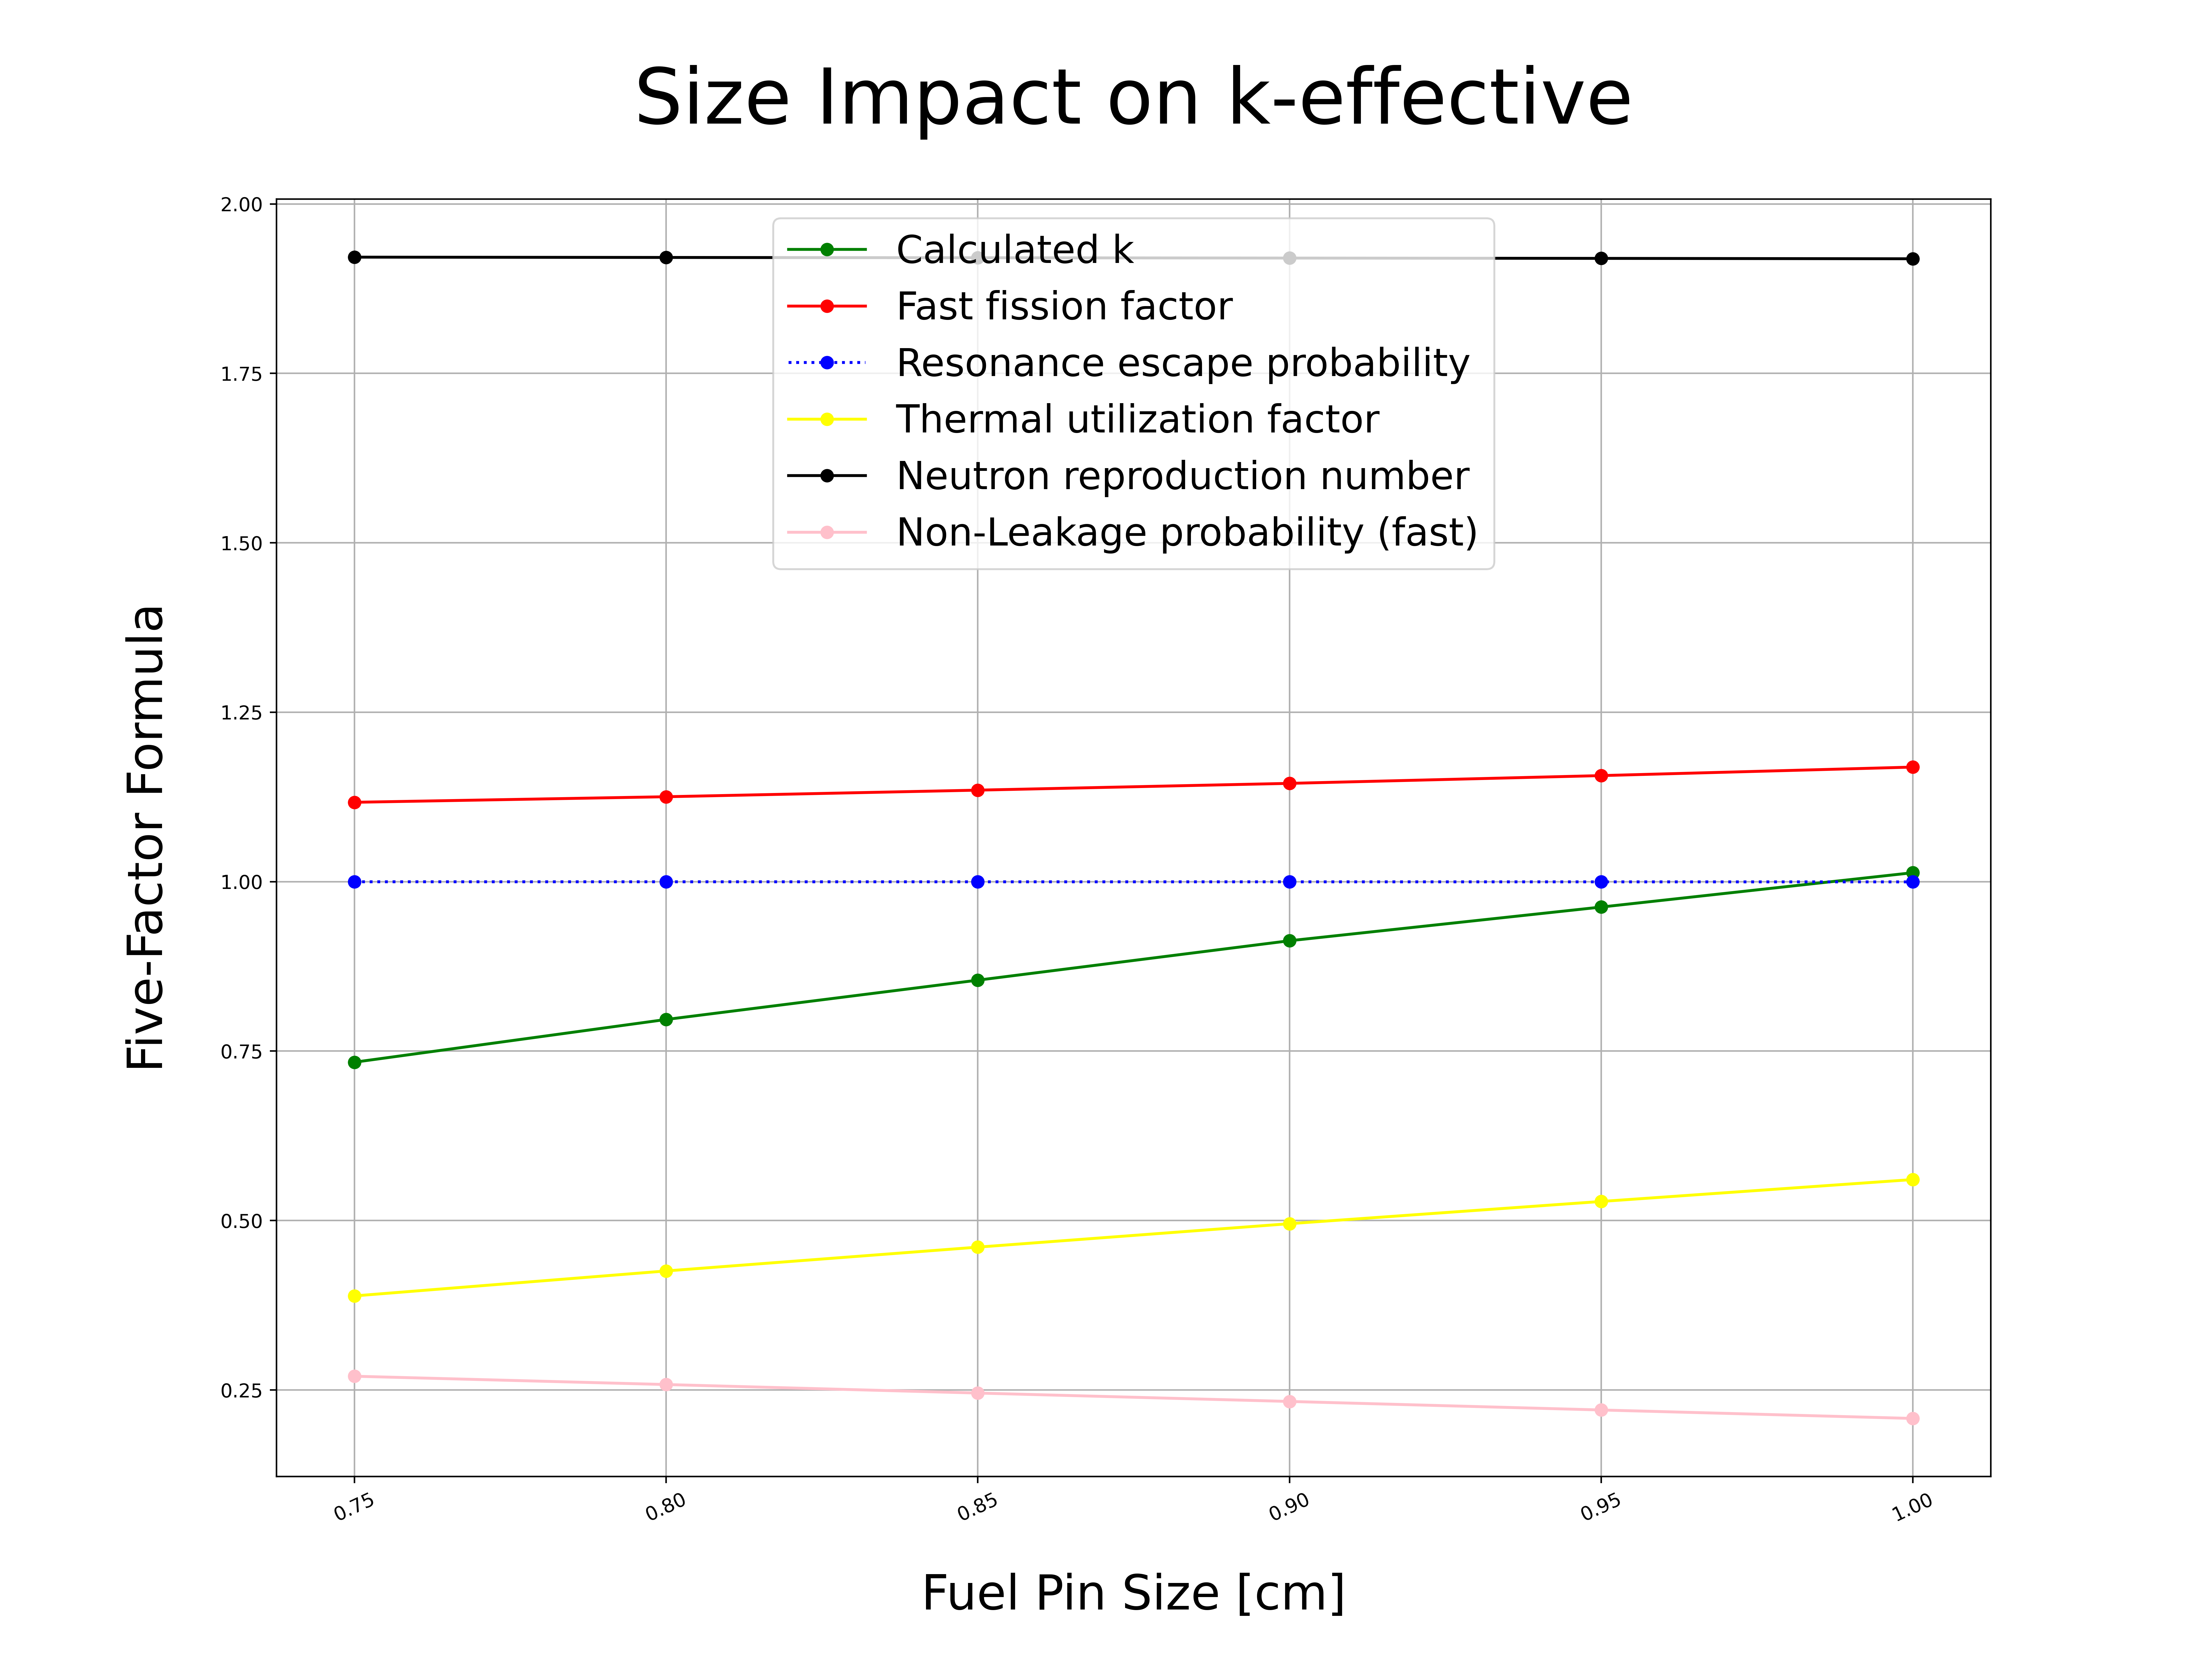
\includegraphics[width=0.35\textwidth]{../Pin_Cell/Light_Water.png}
  \caption{Five-factor formula coefficients for a pin cell with light water moderator.}
  \label{fig:FFFlight}
\end{figure}

\begin{figure}[ht]
  \centering
  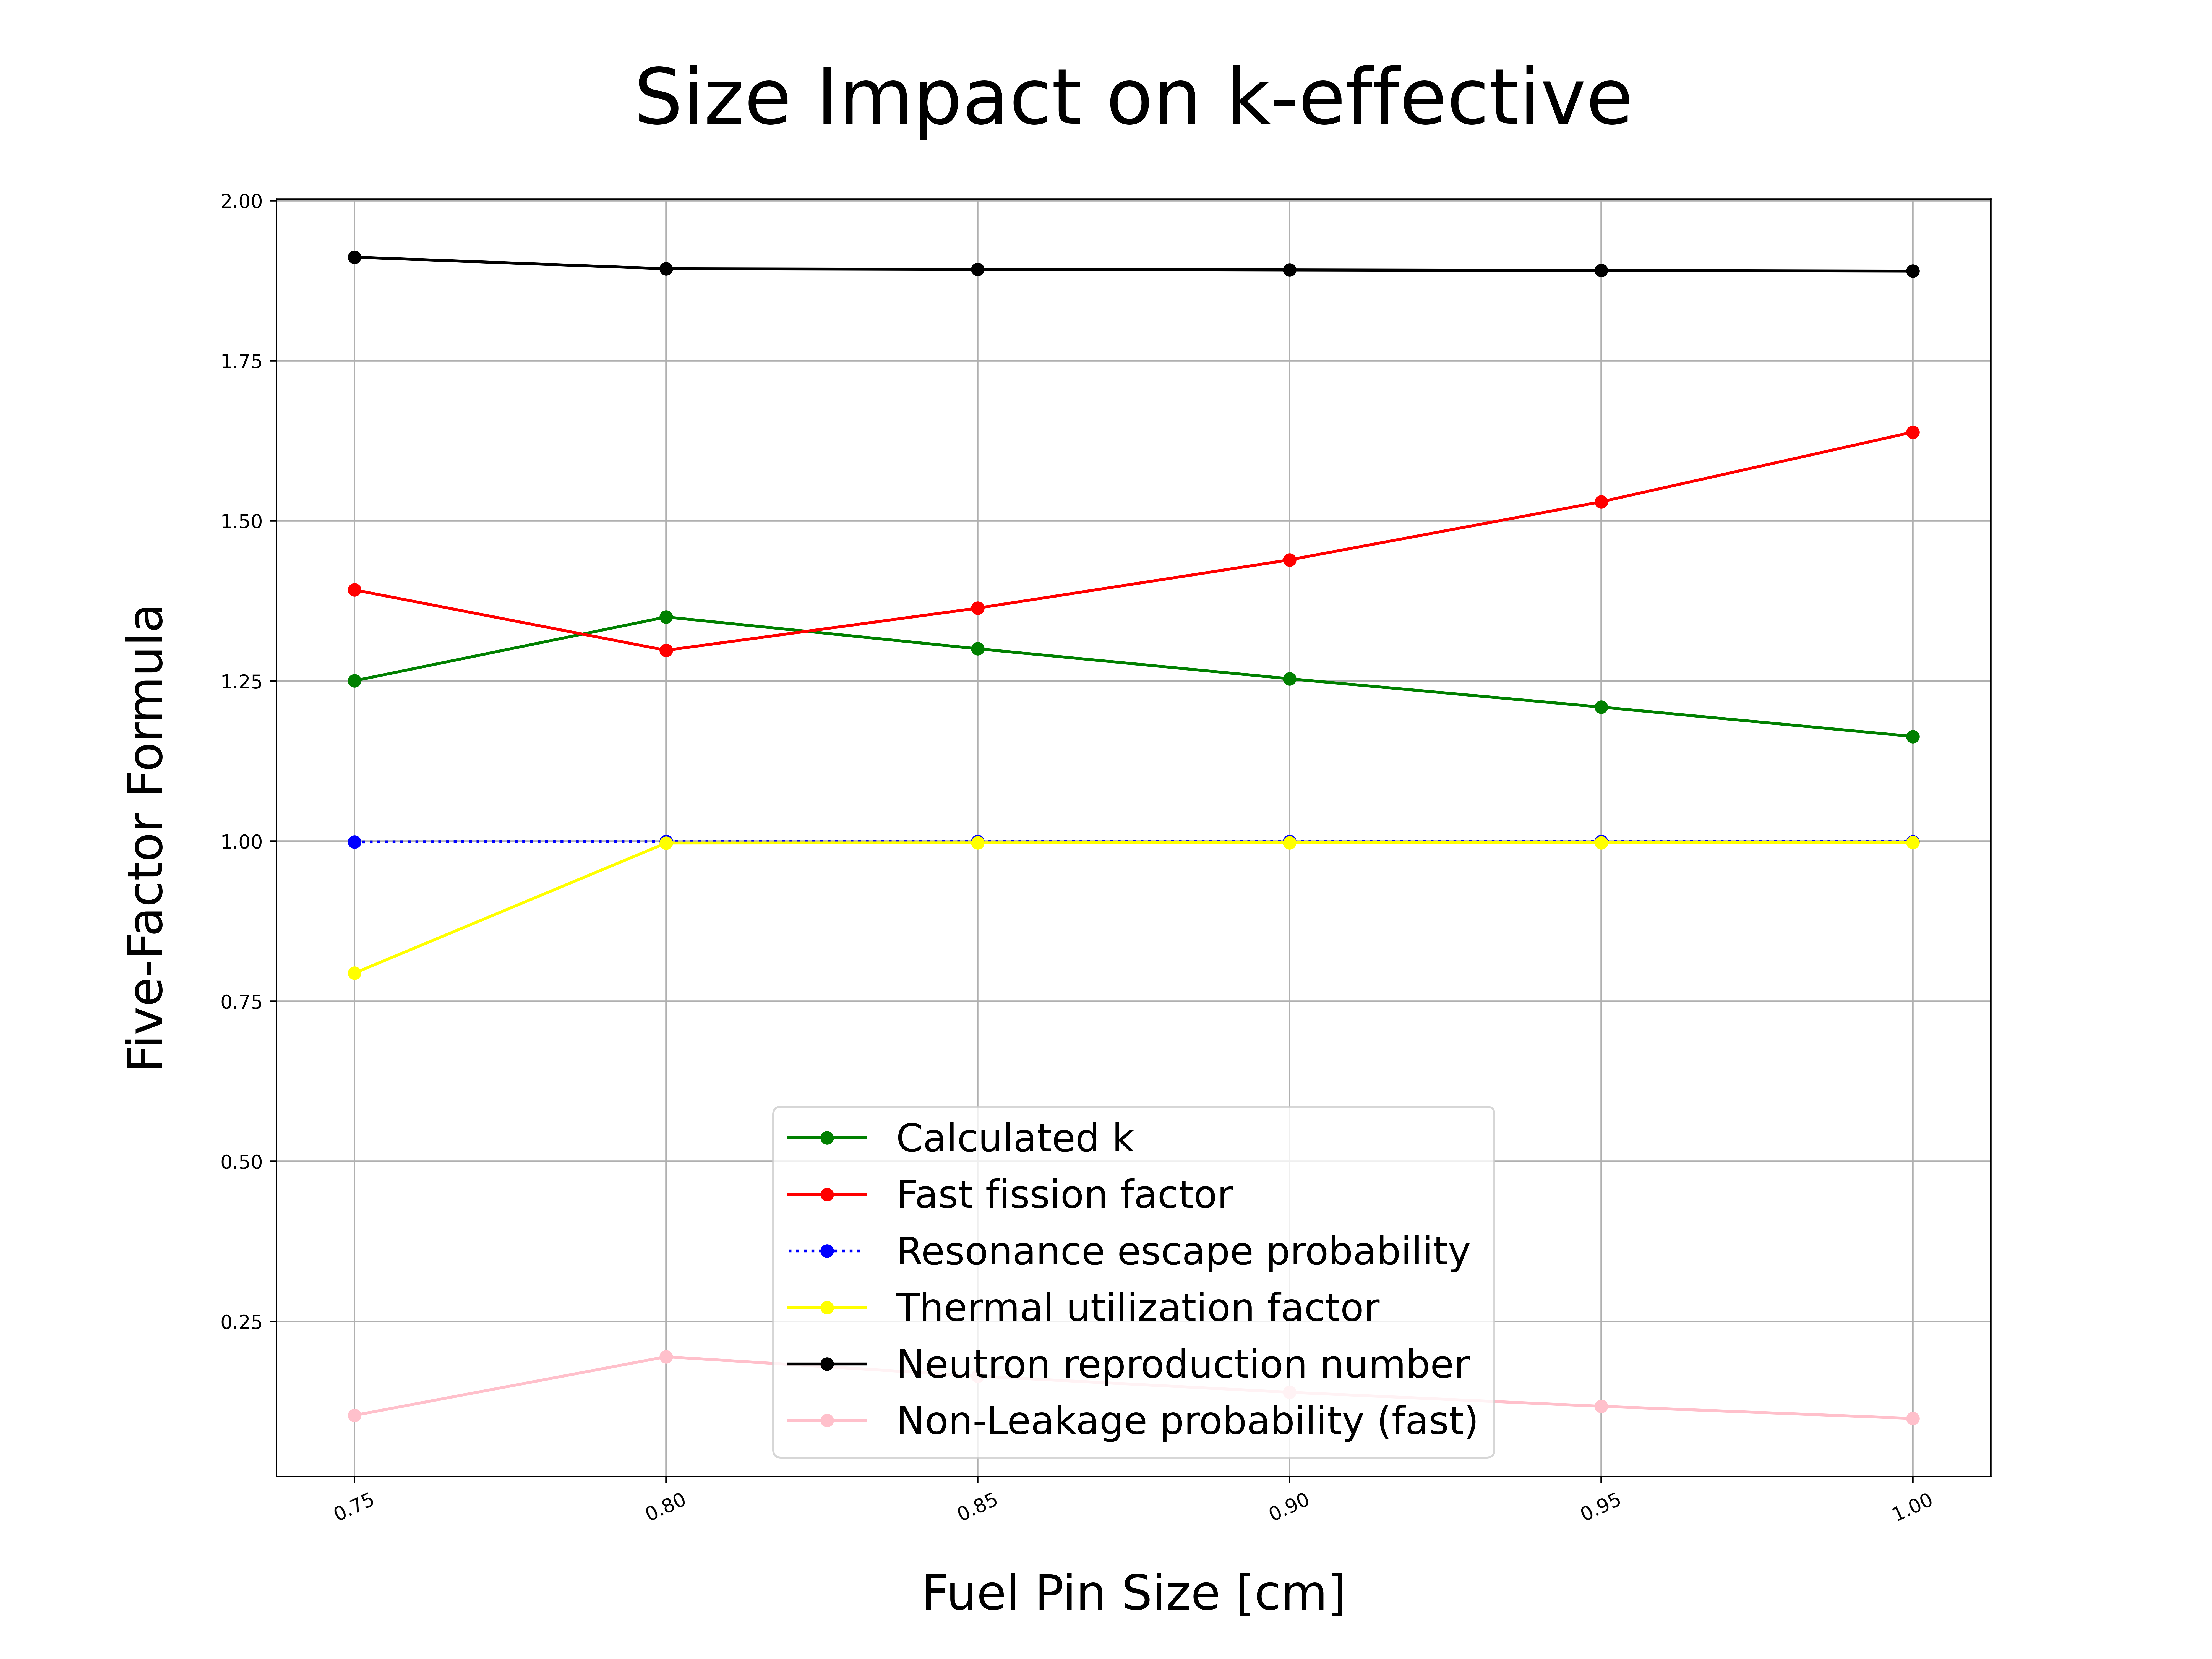
\includegraphics[width=0.35\textwidth]{../Pin_Cell/Heavy_Water.png}
  \caption{Five-factor formula coefficients for a pin cell with heavy water moderator.}
  \label{fig:FFFheavy}
\end{figure}

\begin{figure}[ht]
  \centering
  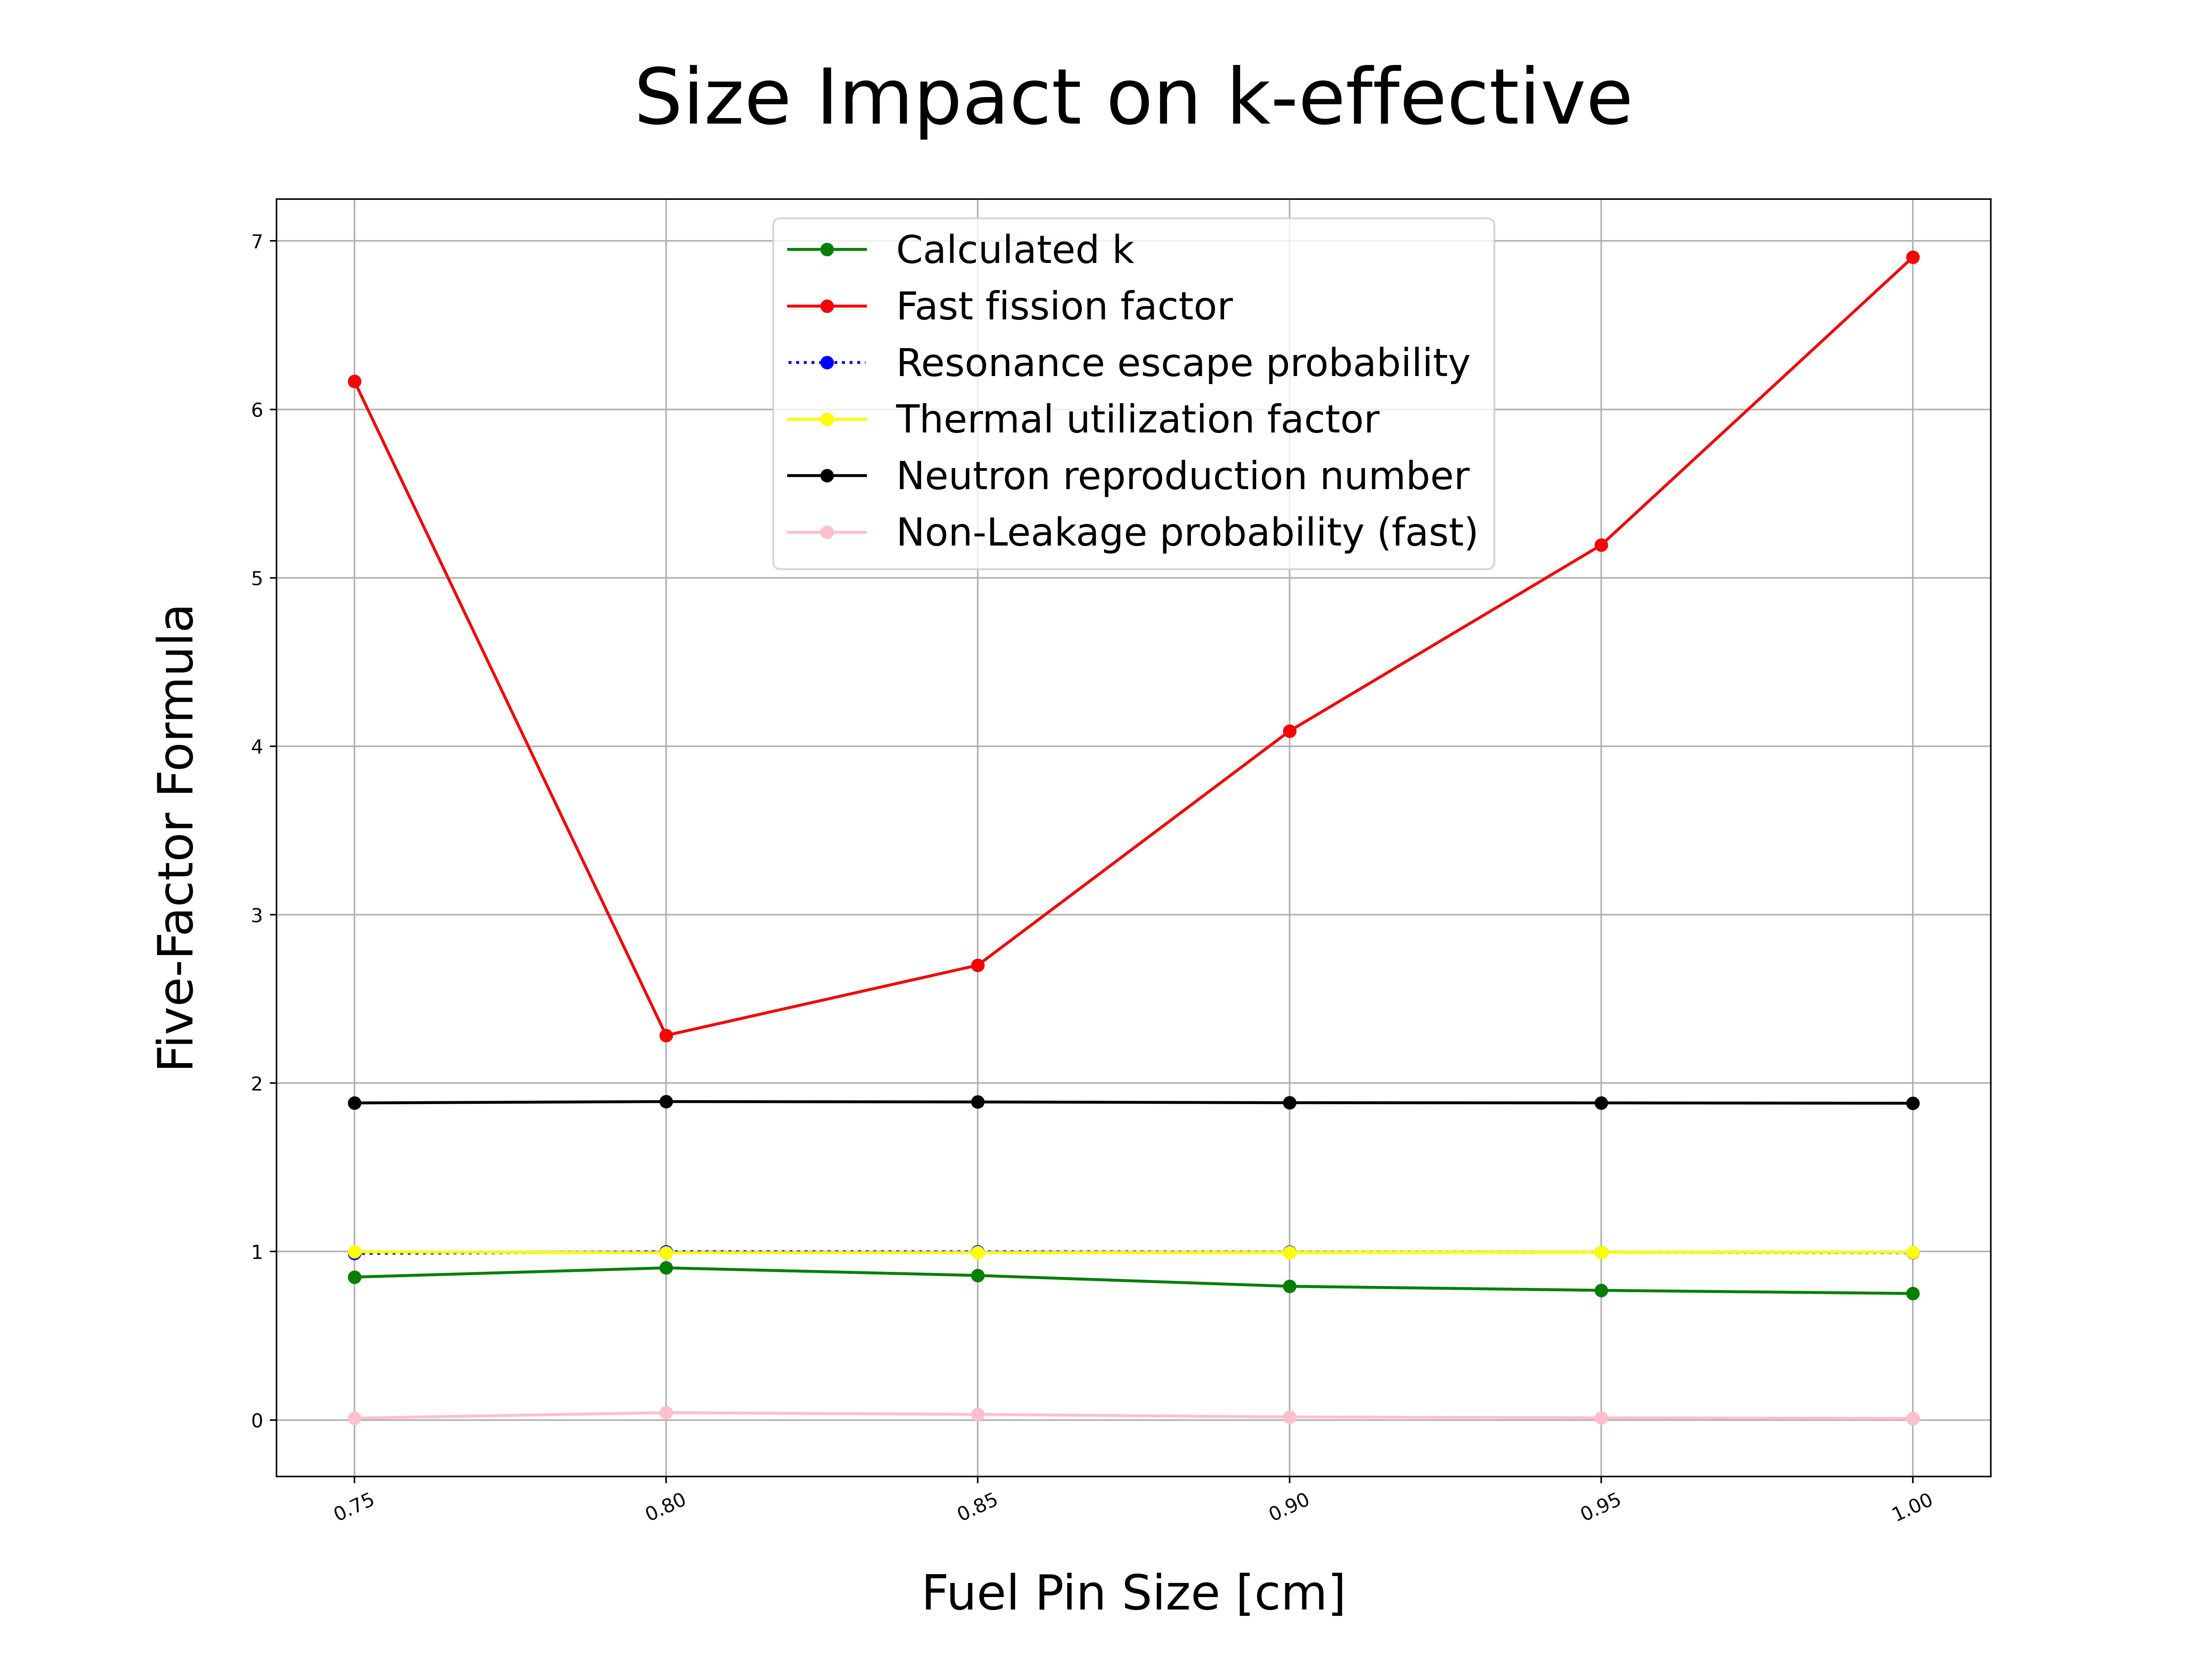
\includegraphics[width=0.35\textwidth]{../Pin_Cell/Graphite.png}
  \caption{Five-factor formula coefficients for a pin cell with graphite moderator.}
  \label{fig:FFFgraphite}
\end{figure}

\begin{figure}[ht]
  \centering
  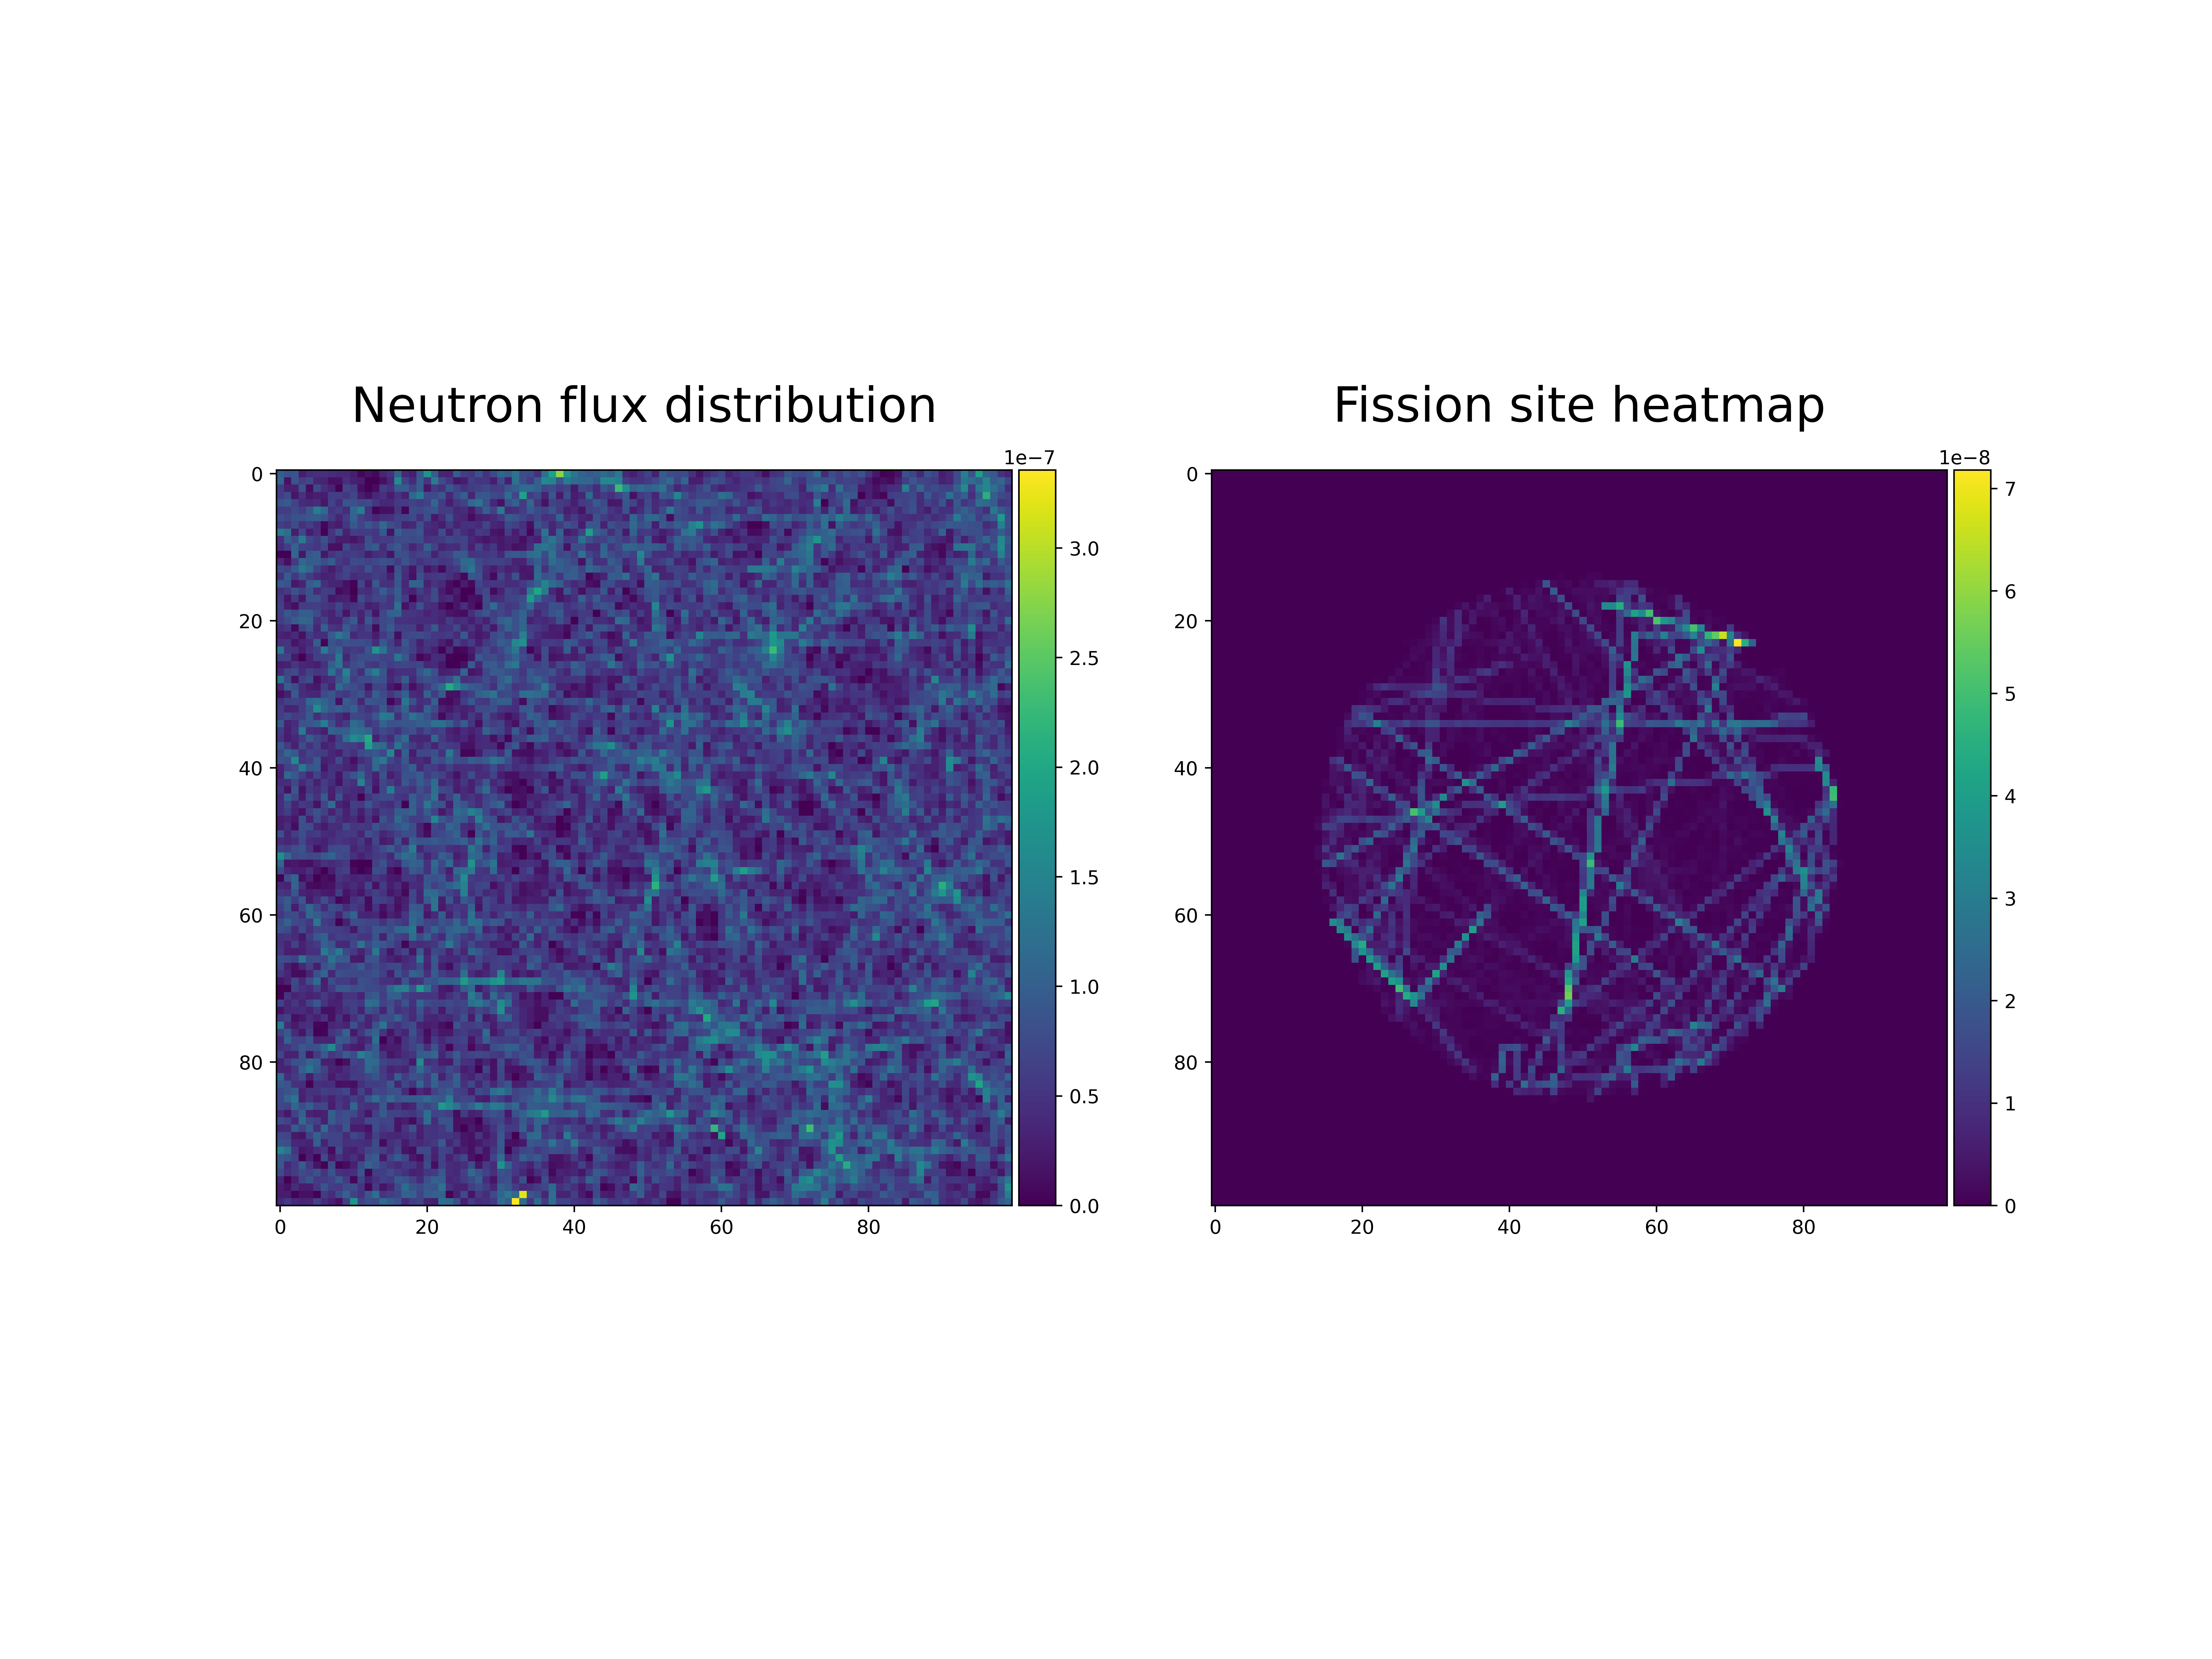
\includegraphics[width=0.4\textwidth]{../Pictures/Mesh_Fuel_Pin_Cell.png}
  \caption{Neutron flux distribution and fission site heatmap for the reactor fuel pin cell.}
  \label{fig:meshfuel}
\end{figure}

\begin{figure}[ht]
  \centering
  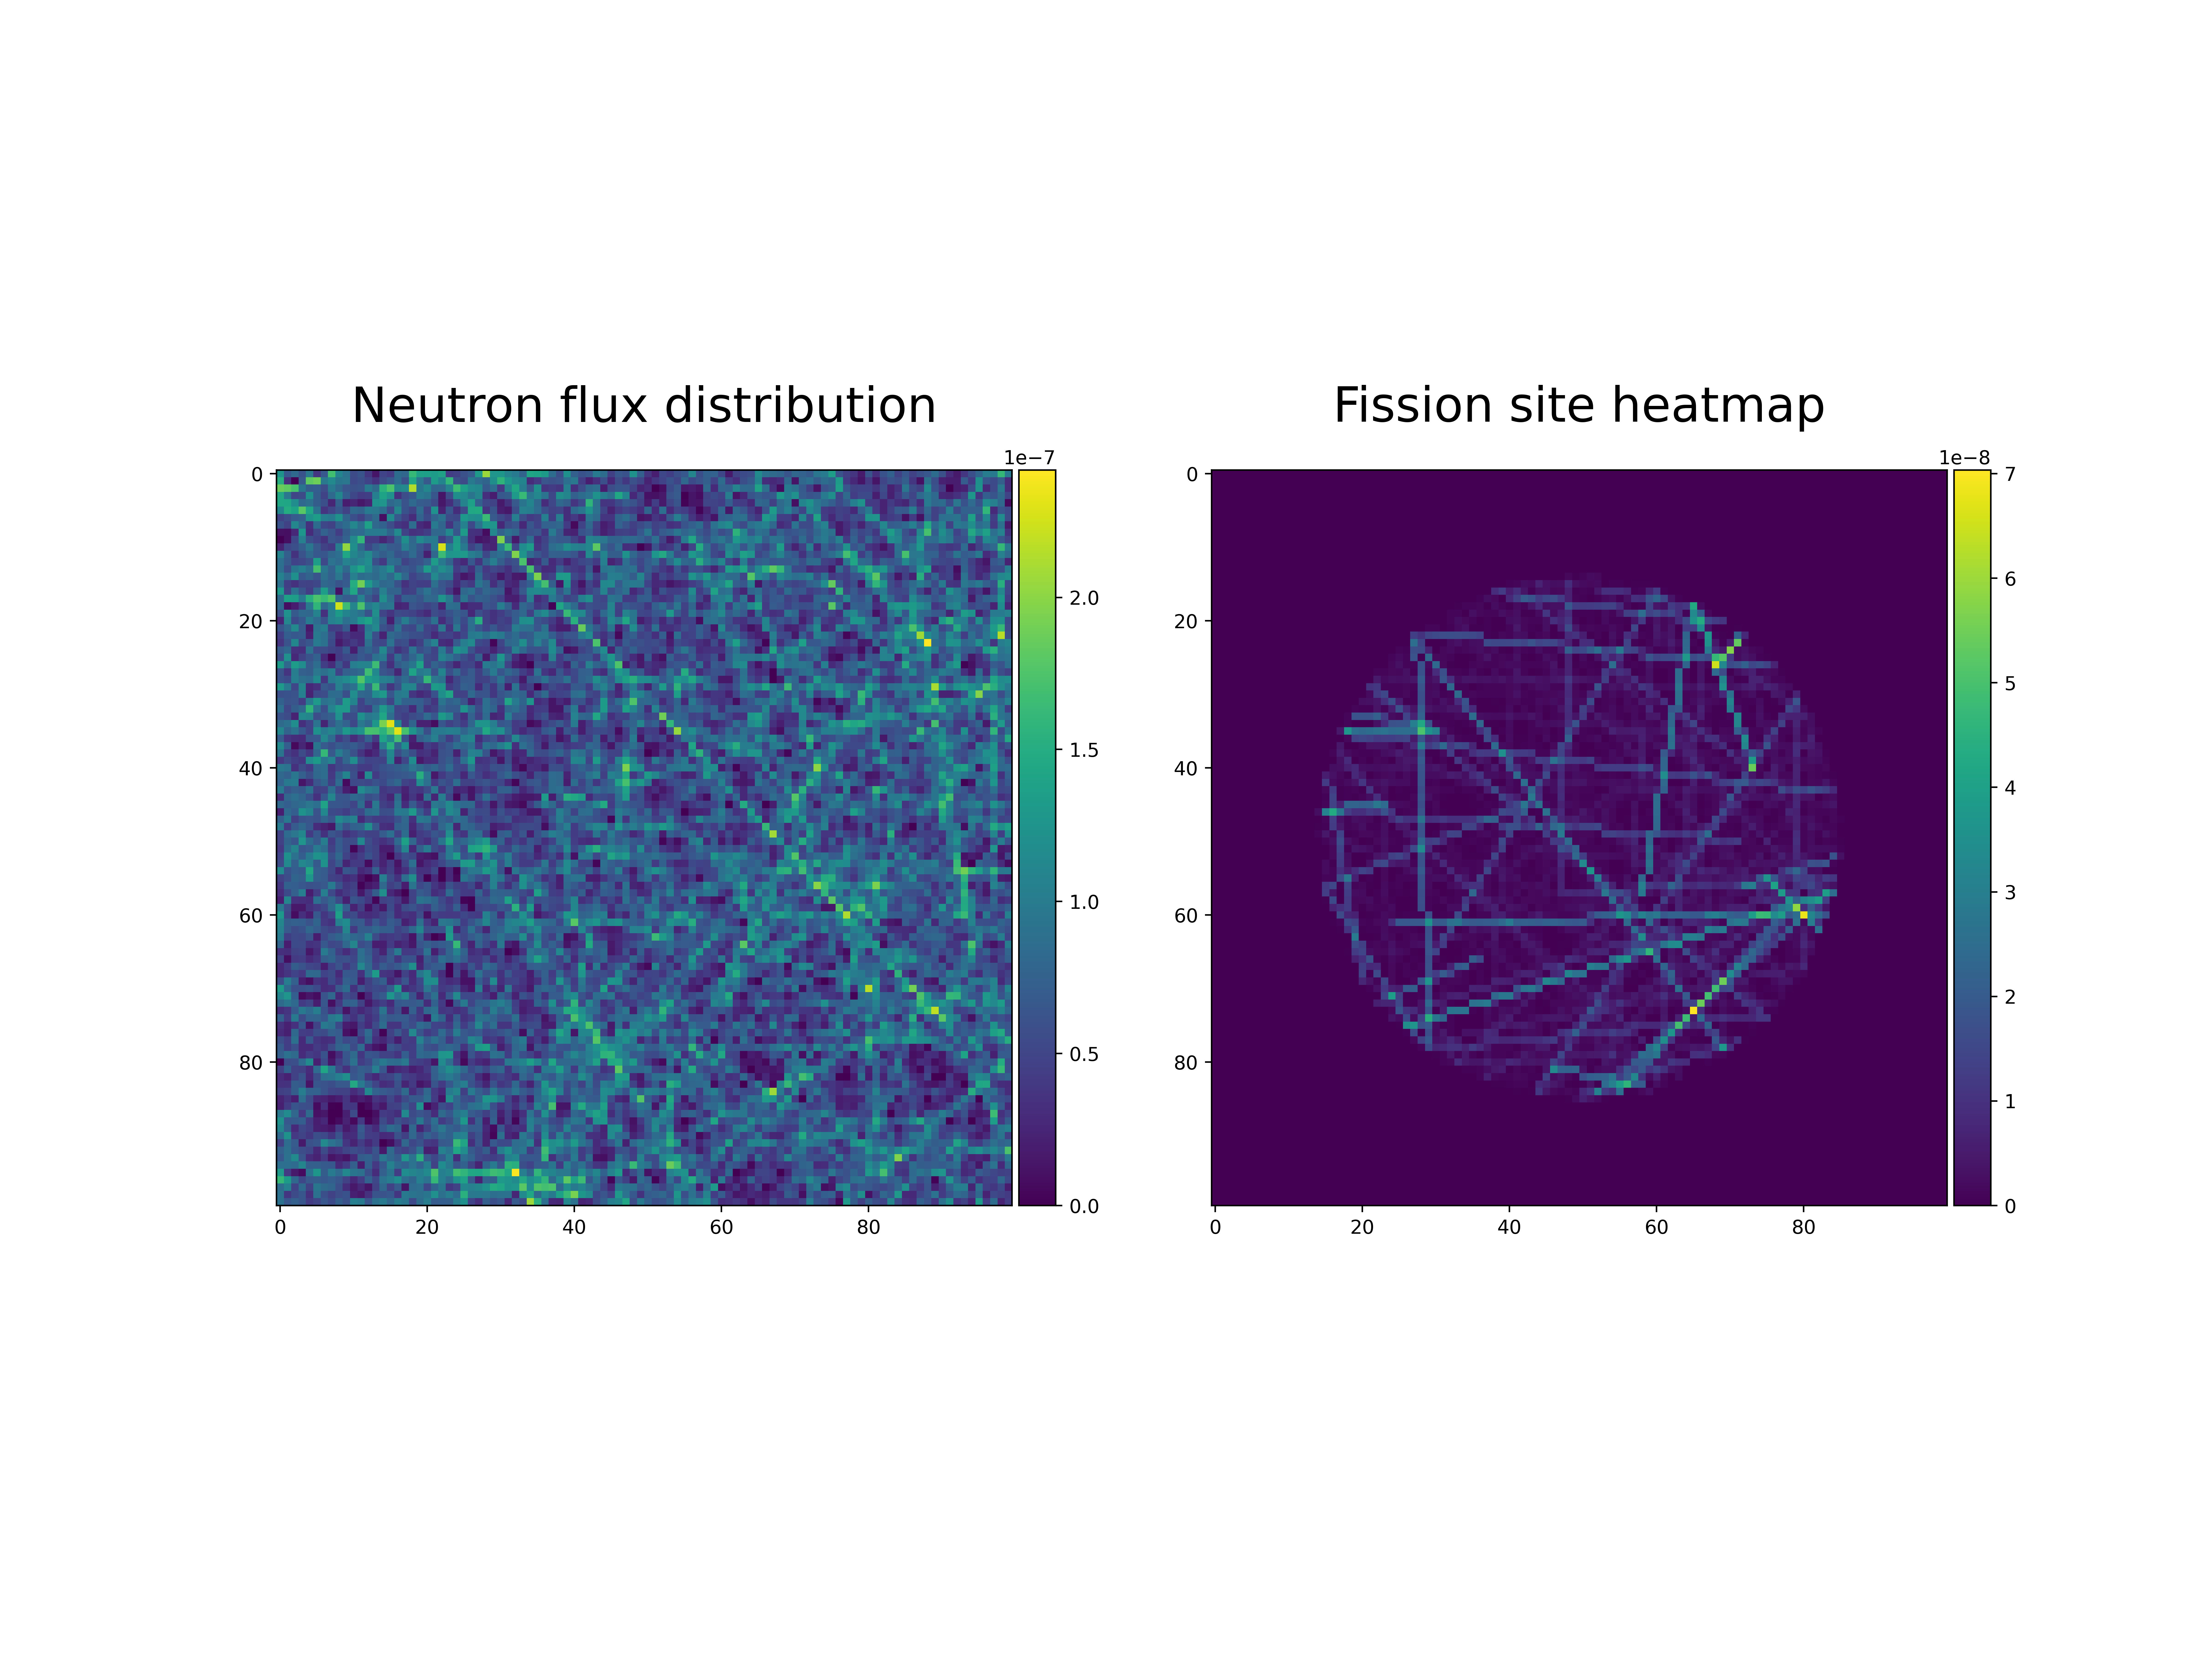
\includegraphics[width=0.4\textwidth]{../Pictures/Mesh_Burnable_Fuel_Pin_Cell.png}
  \caption{Neutron flux distribution and fission site heatmap for the reactor burnable fuel pin cell.}
  \label{fig:meshburn}
\end{figure}

\begin{figure}[ht]
  \centering
  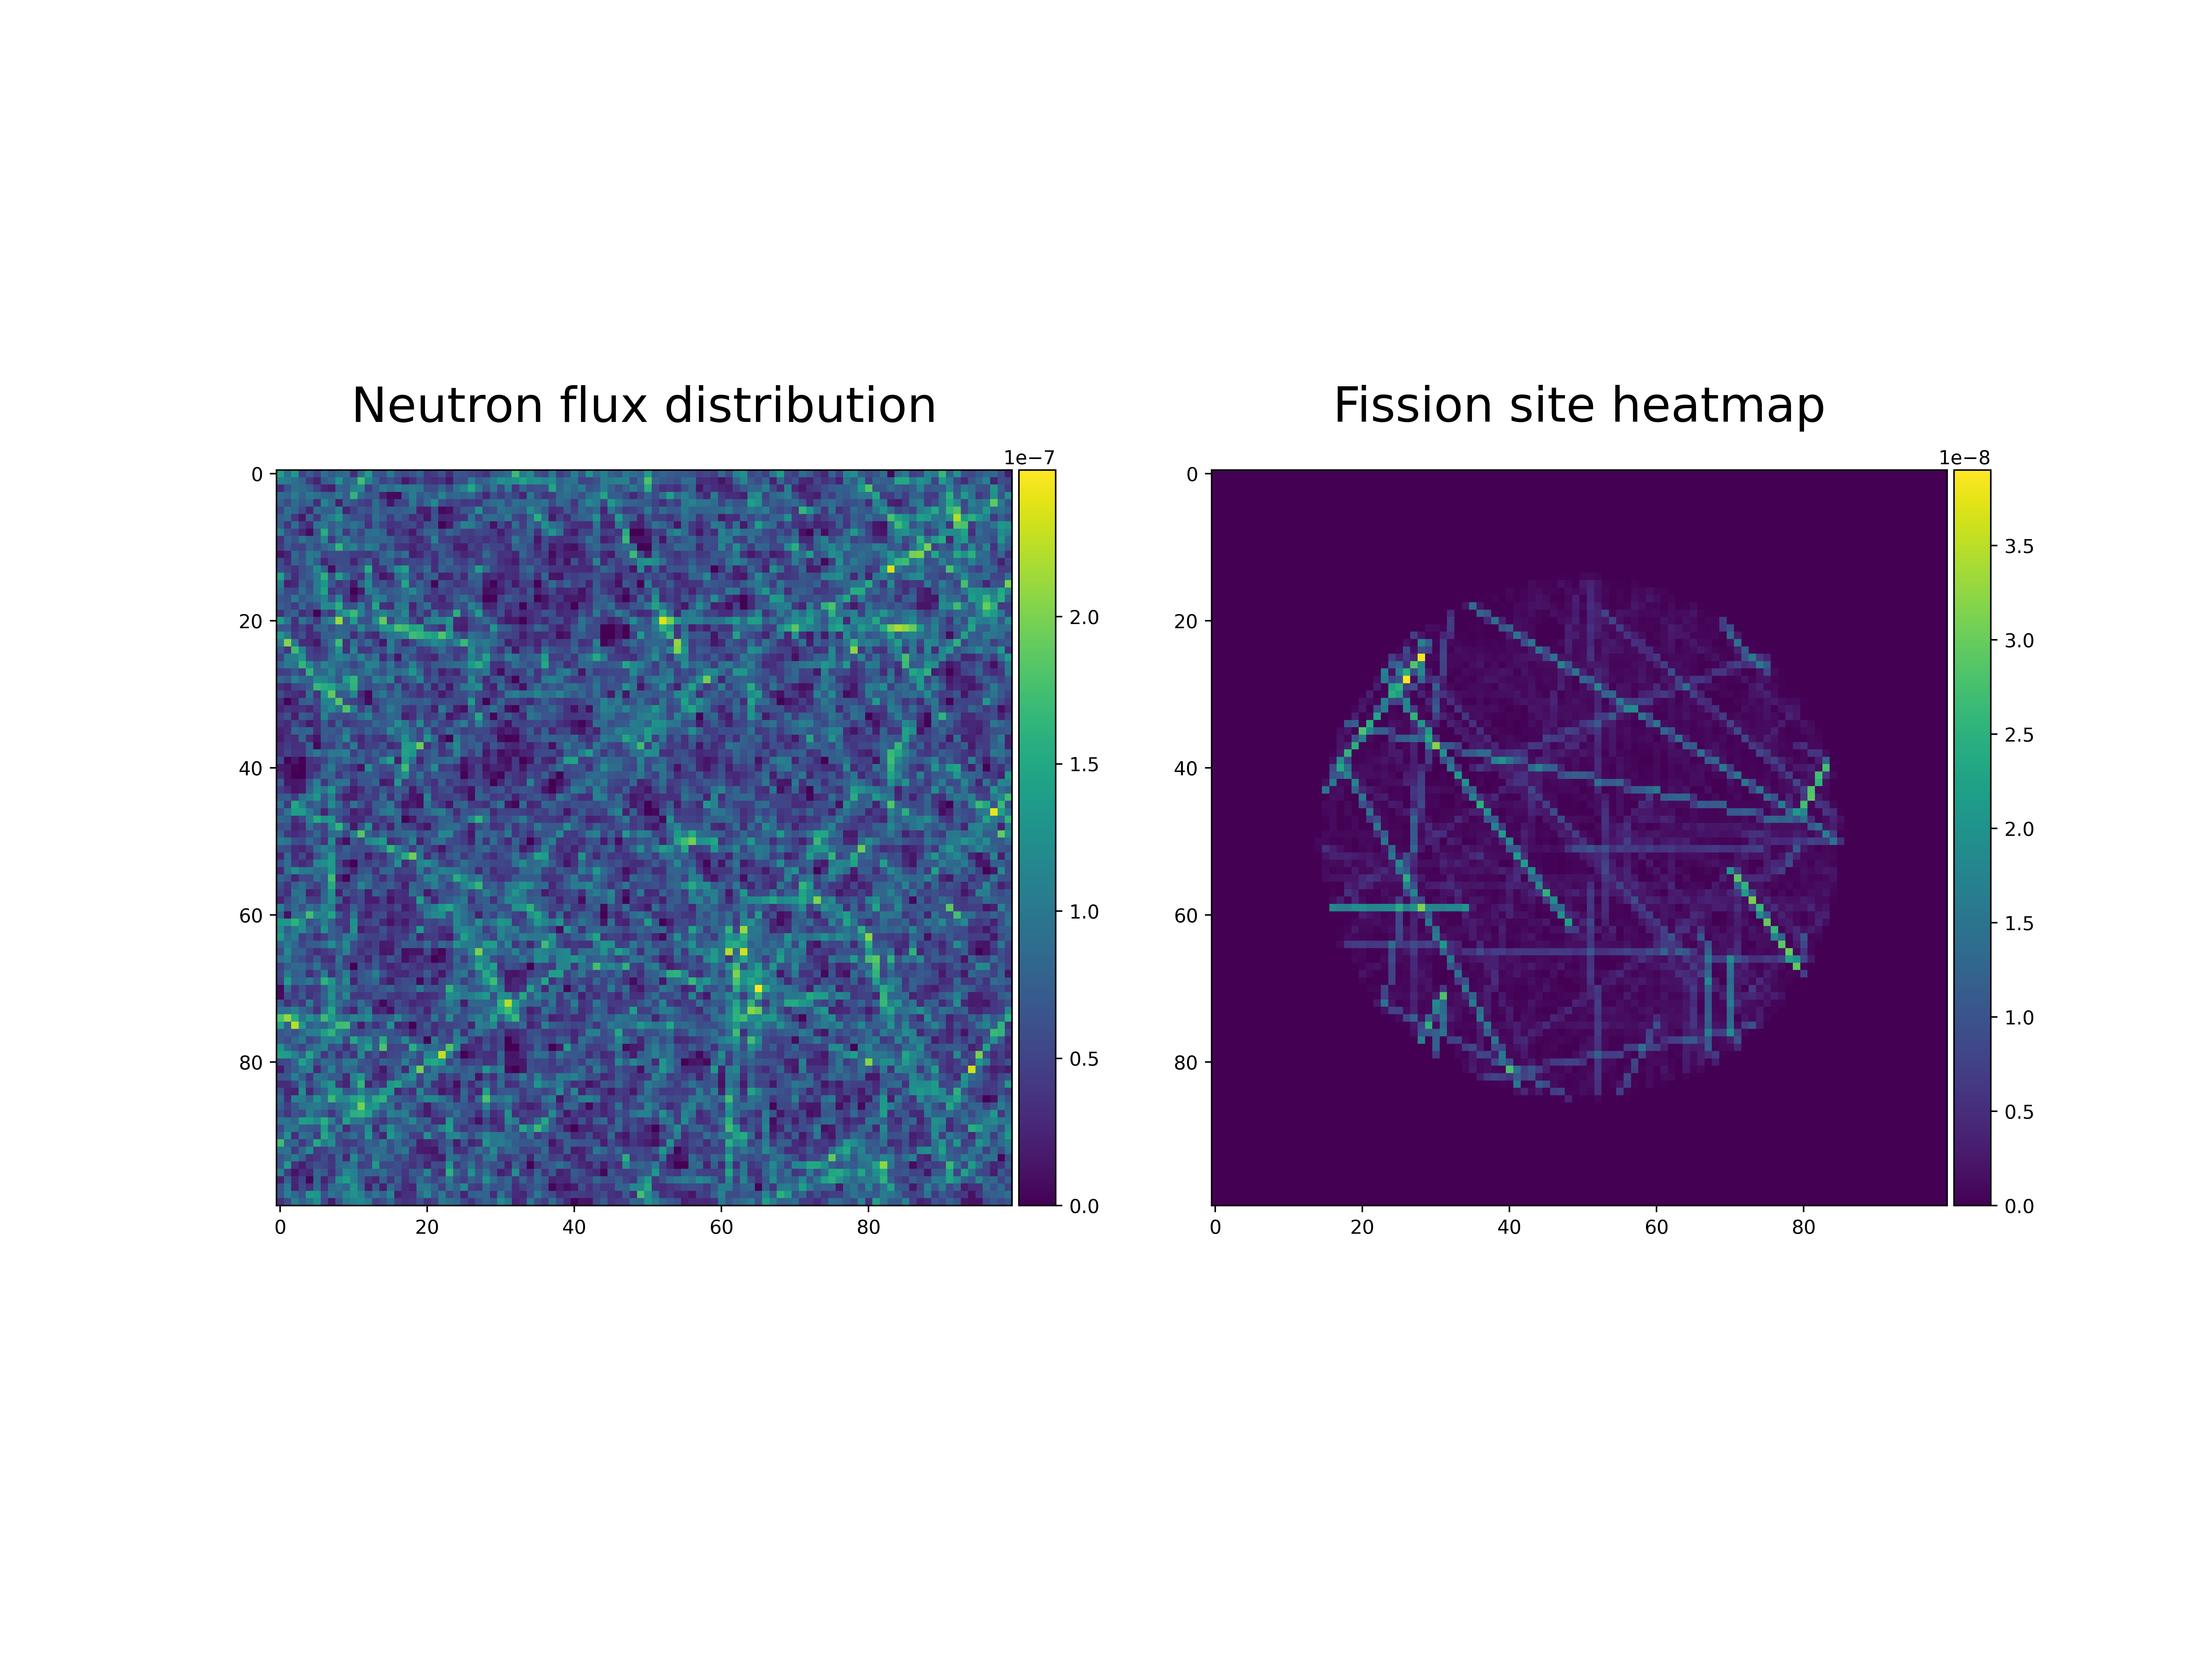
\includegraphics[width=0.4\textwidth]{../Pictures/Mesh_Control_Pin_Cell.png}
  \caption{Neutron flux distribution and fission site heatmap for the reactor control pin cell.}
  \label{fig:meshcont}
\end{figure}

\begin{figure}[ht]
  \centering
  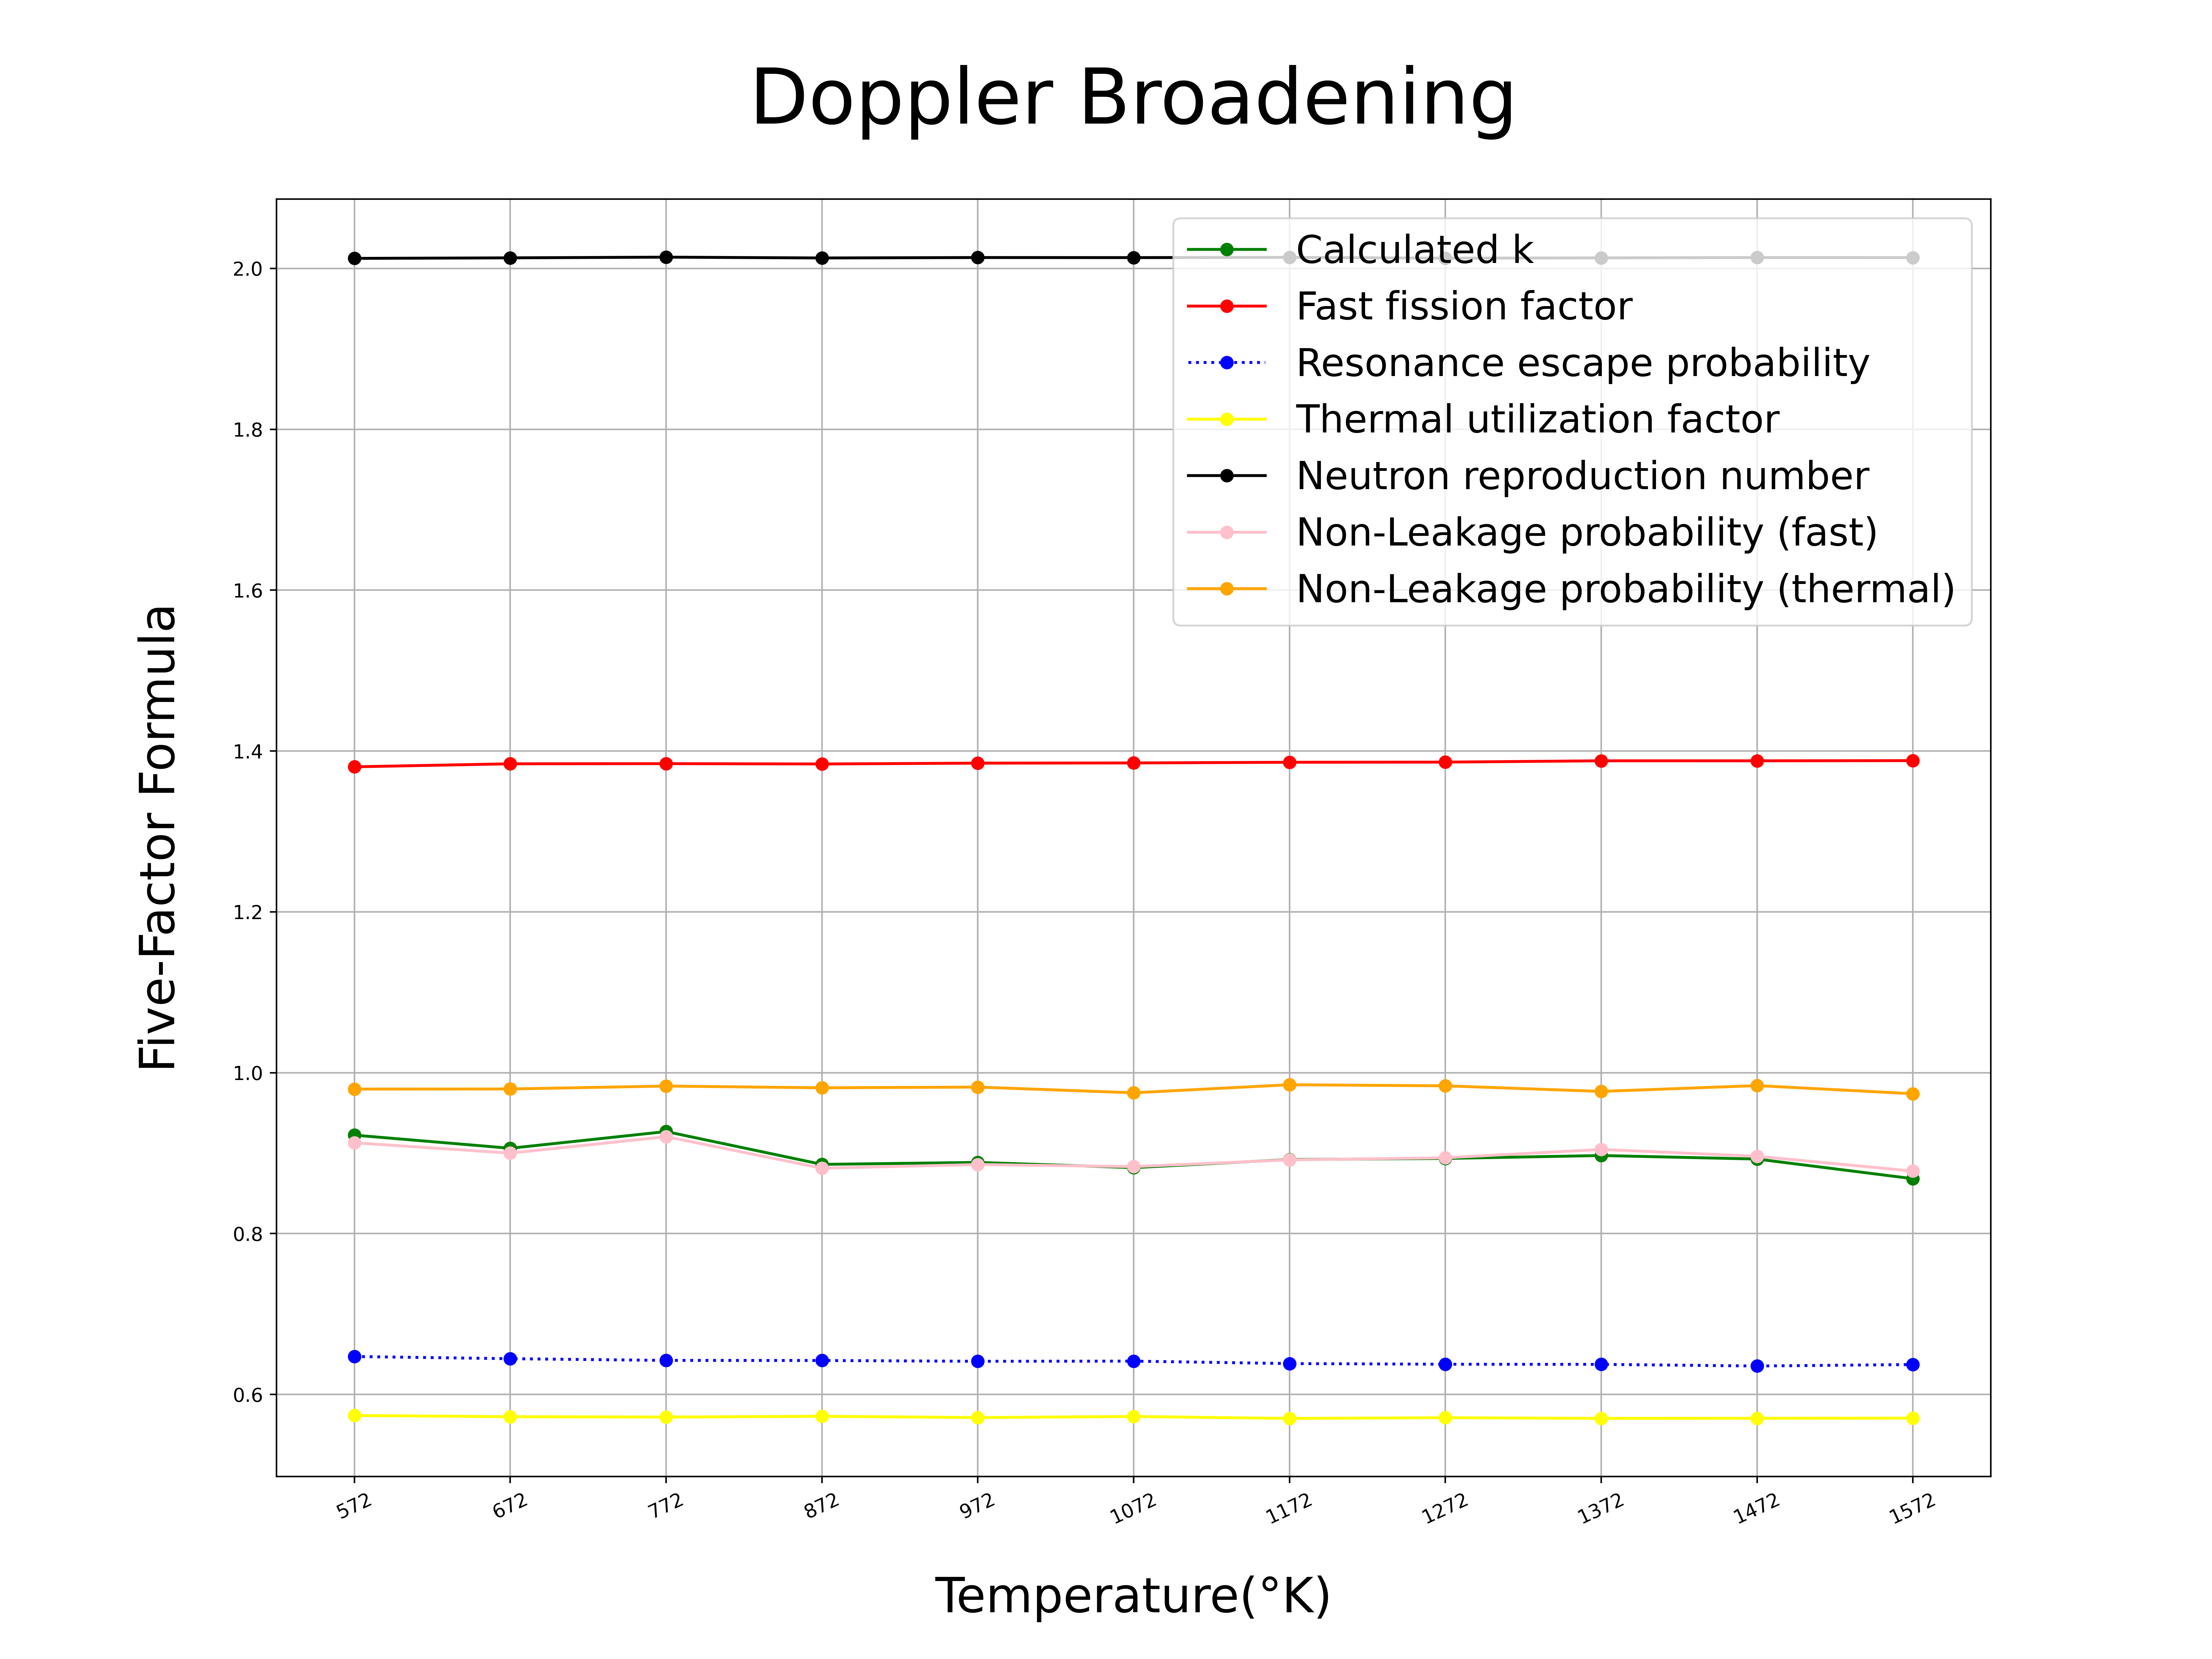
\includegraphics[width=0.4\textwidth]{../Pictures/Doppler_Five.png}
  \caption{Five-factor formula coefficients as function of increasing temperature.}
  \label{fig:Dopp5FF}
\end{figure}

\begin{figure}[ht]
  \centering
  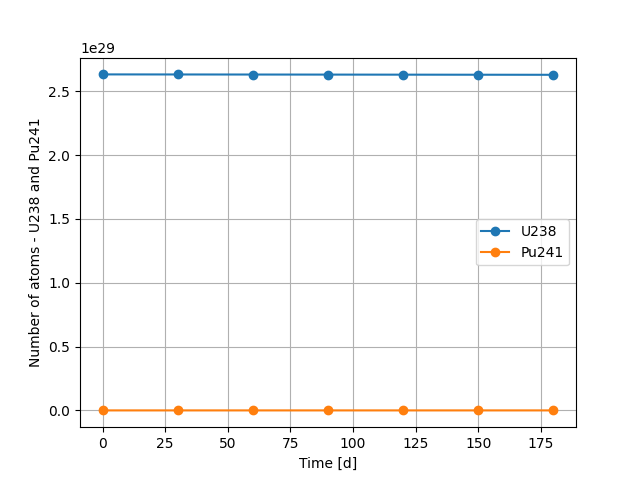
\includegraphics[width=0.4\textwidth]{../Pictures/Depletion_U238_Pu241.png}
  \caption{Decreasing k-effective as temperature increases due to Doppler broadening.}
  \label{fig:U238vsPu241}
\end{figure}

\begin{figure}[ht]
  \centering
  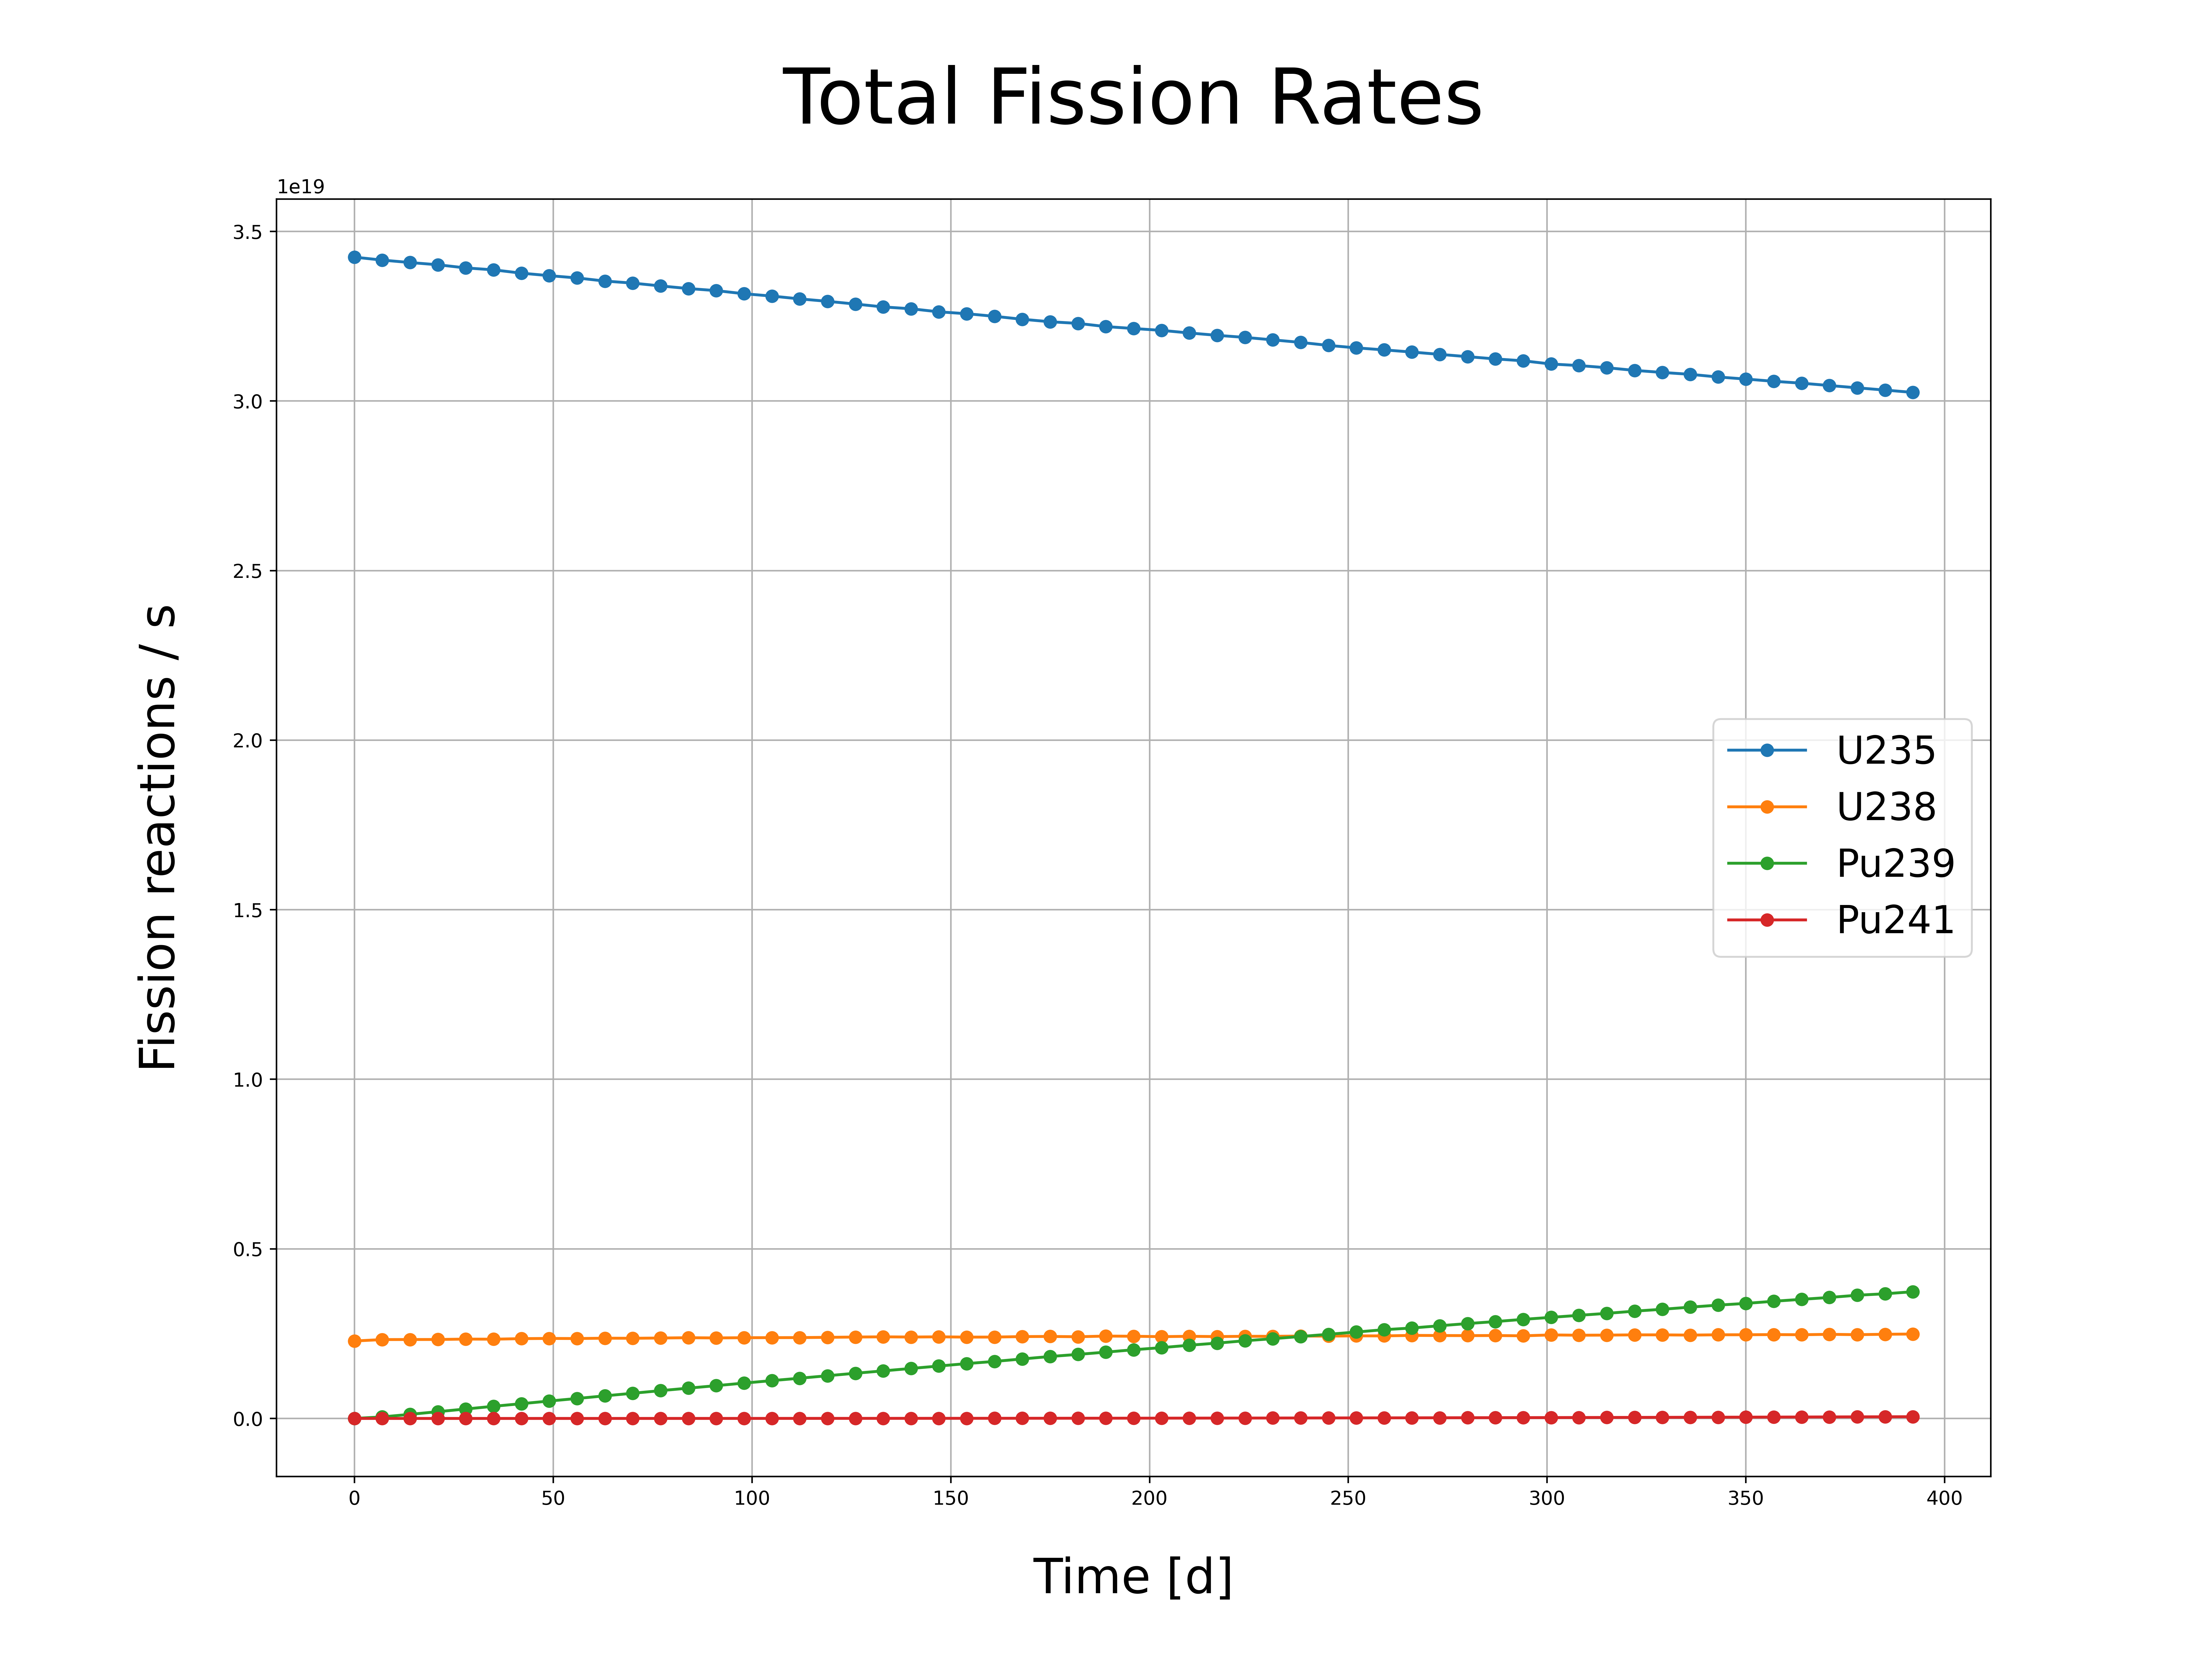
\includegraphics[width=0.4\textwidth]{../Pictures/Depletion_Fission.png}
  \caption{Decreasing k-effective as temperature increases due to Doppler broadening.}
  \label{fig:totalfission}
\end{figure}

\end{document}

%####################################################################################################################################################
% END
%####################################################################################################################################################